\providecommand{\qRobotColorMediumPlot}{
\begin{figure}[!ht]
	\centering
	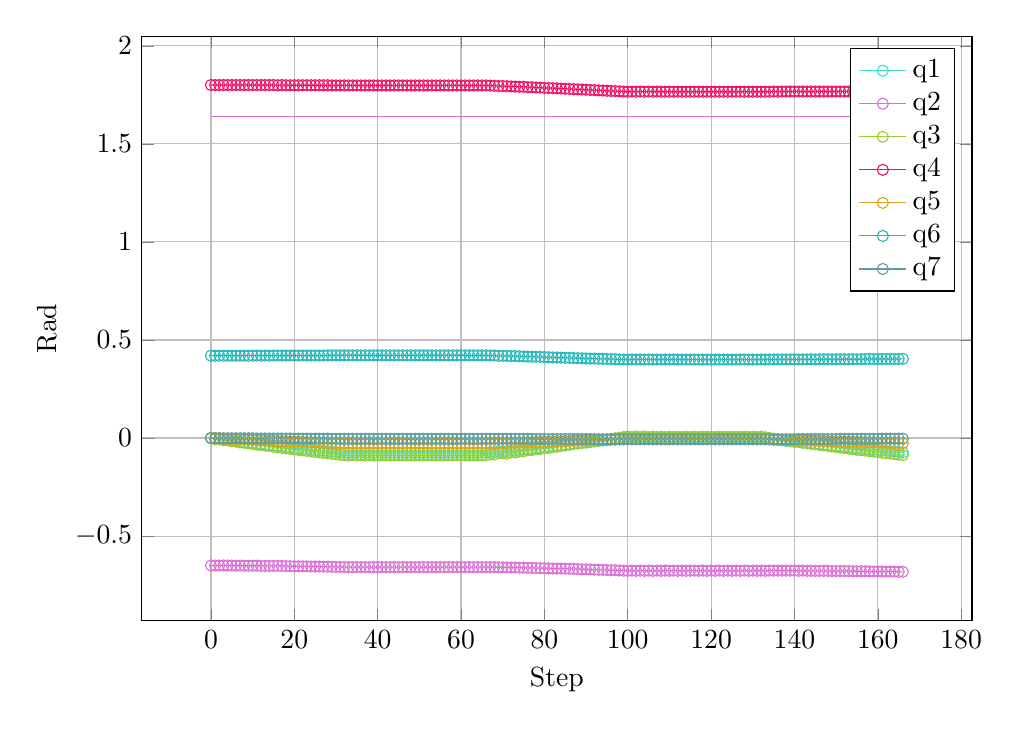
\begin{tikzpicture}
		\begin{axis}[height=9cm, width=\textwidth, grid=major,
		xlabel={Step},ylabel={Rad}
		]
			\addplot [color=Turquoise, mark=o] coordinates {
				(0, 0.000)
				(1, -0.005)
				(2, -0.005)
				(3, -0.010)
				(4, -0.010)
				(5, -0.014)
				(6, -0.015)
				(7, -0.019)
				(8, -0.020)
				(9, -0.024)
				(10, -0.025)
				(11, -0.029)
				(12, -0.030)
				(13, -0.034)
				(14, -0.035)
				(15, -0.038)
				(16, -0.040)
				(17, -0.043)
				(18, -0.045)
				(19, -0.047)
				(20, -0.049)
				(21, -0.052)
				(22, -0.054)
				(23, -0.056)
				(24, -0.058)
				(25, -0.061)
				(26, -0.063)
				(27, -0.065)
				(28, -0.067)
				(29, -0.070)
				(30, -0.071)
				(31, -0.074)
				(32, -0.075)
				(33, -0.077)
				(34, -0.075)
				(35, -0.077)
				(36, -0.074)
				(37, -0.077)
				(38, -0.075)
				(39, -0.077)
				(40, -0.075)
				(41, -0.077)
				(42, -0.075)
				(43, -0.076)
				(44, -0.075)
				(45, -0.076)
				(46, -0.075)
				(47, -0.076)
				(48, -0.075)
				(49, -0.076)
				(50, -0.075)
				(51, -0.076)
				(52, -0.075)
				(53, -0.076)
				(54, -0.076)
				(55, -0.076)
				(56, -0.076)
				(57, -0.075)
				(58, -0.076)
				(59, -0.075)
				(60, -0.076)
				(61, -0.075)
				(62, -0.076)
				(63, -0.075)
				(64, -0.076)
				(65, -0.075)
				(66, -0.076)
				(67, -0.071)
				(68, -0.072)
				(69, -0.067)
				(70, -0.068)
				(71, -0.068)
				(72, -0.063)
				(73, -0.064)
				(74, -0.059)
				(75, -0.059)
				(76, -0.055)
				(77, -0.055)
				(78, -0.050)
				(79, -0.050)
				(80, -0.046)
				(81, -0.045)
				(82, -0.041)
				(83, -0.040)
				(84, -0.037)
				(85, -0.036)
				(86, -0.032)
				(87, -0.029)
				(88, -0.027)
				(89, -0.025)
				(90, -0.023)
				(91, -0.020)
				(92, -0.018)
				(93, -0.016)
				(94, -0.013)
				(95, -0.011)
				(96, -0.009)
				(97, -0.006)
				(98, -0.004)
				(99, -0.002)
				(100, 0.000)
				(101, -0.002)
				(102, 0.000)
				(103, -0.002)
				(104, 0.000)
				(105, -0.002)
				(106, -0.000)
				(107, -0.002)
				(108, 0.000)
				(109, -0.002)
				(110, -0.000)
				(111, -0.001)
				(112, -0.000)
				(113, -0.001)
				(114, -0.000)
				(115, -0.001)
				(116, -0.000)
				(117, -0.001)
				(118, -0.000)
				(119, -0.001)
				(120, -0.000)
				(121, -0.001)
				(122, -0.000)
				(123, -0.001)
				(124, -0.000)
				(125, -0.001)
				(126, -0.000)
				(127, -0.001)
				(128, -0.000)
				(129, -0.001)
				(130, -0.001)
				(131, -0.001)
				(132, -0.001)
				(133, -0.002)
				(134, -0.005)
				(135, -0.008)
				(136, -0.010)
				(137, -0.012)
				(138, -0.015)
				(139, -0.017)
				(140, -0.019)
				(141, -0.021)
				(142, -0.024)
				(143, -0.026)
				(144, -0.028)
				(145, -0.030)
				(146, -0.032)
				(147, -0.035)
				(148, -0.037)
				(149, -0.039)
				(150, -0.041)
				(151, -0.043)
				(152, -0.045)
				(153, -0.048)
				(154, -0.049)
				(155, -0.052)
				(156, -0.053)
				(157, -0.055)
				(158, -0.058)
				(159, -0.059)
				(160, -0.061)
				(161, -0.063)
				(162, -0.065)
				(163, -0.067)
				(164, -0.069)
				(165, -0.071)
				(166, -0.073)
			};
			\addlegendentry{q1}

			\addplot [color=Orchid, mark=o] coordinates {
				(0, -0.650)
				(1, -0.650)
				(2, -0.650)
				(3, -0.650)
				(4, -0.650)
				(5, -0.650)
				(6, -0.651)
				(7, -0.650)
				(8, -0.651)
				(9, -0.651)
				(10, -0.651)
				(11, -0.651)
				(12, -0.652)
				(13, -0.652)
				(14, -0.652)
				(15, -0.652)
				(16, -0.652)
				(17, -0.652)
				(18, -0.653)
				(19, -0.653)
				(20, -0.654)
				(21, -0.654)
				(22, -0.654)
				(23, -0.654)
				(24, -0.655)
				(25, -0.655)
				(26, -0.655)
				(27, -0.656)
				(28, -0.656)
				(29, -0.657)
				(30, -0.657)
				(31, -0.657)
				(32, -0.658)
				(33, -0.658)
				(34, -0.658)
				(35, -0.658)
				(36, -0.658)
				(37, -0.658)
				(38, -0.658)
				(39, -0.658)
				(40, -0.658)
				(41, -0.658)
				(42, -0.658)
				(43, -0.658)
				(44, -0.658)
				(45, -0.658)
				(46, -0.658)
				(47, -0.658)
				(48, -0.658)
				(49, -0.658)
				(50, -0.658)
				(51, -0.658)
				(52, -0.658)
				(53, -0.658)
				(54, -0.658)
				(55, -0.658)
				(56, -0.658)
				(57, -0.658)
				(58, -0.658)
				(59, -0.658)
				(60, -0.658)
				(61, -0.658)
				(62, -0.658)
				(63, -0.658)
				(64, -0.658)
				(65, -0.658)
				(66, -0.658)
				(67, -0.658)
				(68, -0.658)
				(69, -0.659)
				(70, -0.659)
				(71, -0.660)
				(72, -0.660)
				(73, -0.660)
				(74, -0.661)
				(75, -0.661)
				(76, -0.662)
				(77, -0.662)
				(78, -0.663)
				(79, -0.663)
				(80, -0.664)
				(81, -0.664)
				(82, -0.665)
				(83, -0.665)
				(84, -0.666)
				(85, -0.666)
				(86, -0.667)
				(87, -0.667)
				(88, -0.668)
				(89, -0.669)
				(90, -0.669)
				(91, -0.670)
				(92, -0.671)
				(93, -0.672)
				(94, -0.672)
				(95, -0.673)
				(96, -0.674)
				(97, -0.674)
				(98, -0.675)
				(99, -0.676)
				(100, -0.677)
				(101, -0.676)
				(102, -0.677)
				(103, -0.676)
				(104, -0.677)
				(105, -0.676)
				(106, -0.677)
				(107, -0.676)
				(108, -0.677)
				(109, -0.676)
				(110, -0.677)
				(111, -0.676)
				(112, -0.677)
				(113, -0.676)
				(114, -0.677)
				(115, -0.676)
				(116, -0.676)
				(117, -0.677)
				(118, -0.676)
				(119, -0.677)
				(120, -0.676)
				(121, -0.677)
				(122, -0.676)
				(123, -0.677)
				(124, -0.676)
				(125, -0.677)
				(126, -0.676)
				(127, -0.677)
				(128, -0.676)
				(129, -0.677)
				(130, -0.676)
				(131, -0.677)
				(132, -0.676)
				(133, -0.677)
				(134, -0.676)
				(135, -0.676)
				(136, -0.676)
				(137, -0.676)
				(138, -0.676)
				(139, -0.676)
				(140, -0.676)
				(141, -0.677)
				(142, -0.676)
				(143, -0.677)
				(144, -0.677)
				(145, -0.677)
				(146, -0.677)
				(147, -0.677)
				(148, -0.677)
				(149, -0.678)
				(150, -0.678)
				(151, -0.678)
				(152, -0.678)
				(153, -0.678)
				(154, -0.679)
				(155, -0.679)
				(156, -0.679)
				(157, -0.679)
				(158, -0.680)
				(159, -0.680)
				(160, -0.680)
				(161, -0.680)
				(162, -0.681)
				(163, -0.681)
				(164, -0.681)
				(165, -0.682)
				(166, -0.682)
			};
			\addlegendentry{q2}

			\addplot [color=YellowGreen, mark=o] coordinates {
				(0, 0.000)
				(1, -0.006)
				(2, -0.006)
				(3, -0.011)
				(4, -0.012)
				(5, -0.017)
				(6, -0.018)
				(7, -0.023)
				(8, -0.024)
				(9, -0.028)
				(10, -0.030)
				(11, -0.034)
				(12, -0.036)
				(13, -0.039)
				(14, -0.041)
				(15, -0.045)
				(16, -0.047)
				(17, -0.050)
				(18, -0.053)
				(19, -0.055)
				(20, -0.058)
				(21, -0.061)
				(22, -0.063)
				(23, -0.066)
				(24, -0.068)
				(25, -0.071)
				(26, -0.073)
				(27, -0.076)
				(28, -0.078)
				(29, -0.081)
				(30, -0.083)
				(31, -0.086)
				(32, -0.087)
				(33, -0.090)
				(34, -0.087)
				(35, -0.090)
				(36, -0.087)
				(37, -0.090)
				(38, -0.087)
				(39, -0.090)
				(40, -0.088)
				(41, -0.089)
				(42, -0.088)
				(43, -0.089)
				(44, -0.088)
				(45, -0.089)
				(46, -0.088)
				(47, -0.089)
				(48, -0.088)
				(49, -0.089)
				(50, -0.088)
				(51, -0.089)
				(52, -0.088)
				(53, -0.089)
				(54, -0.089)
				(55, -0.089)
				(56, -0.088)
				(57, -0.088)
				(58, -0.089)
				(59, -0.088)
				(60, -0.088)
				(61, -0.088)
				(62, -0.089)
				(63, -0.088)
				(64, -0.089)
				(65, -0.088)
				(66, -0.089)
				(67, -0.083)
				(68, -0.084)
				(69, -0.077)
				(70, -0.078)
				(71, -0.080)
				(72, -0.073)
				(73, -0.074)
				(74, -0.068)
				(75, -0.068)
				(76, -0.062)
				(77, -0.062)
				(78, -0.057)
				(79, -0.056)
				(80, -0.051)
				(81, -0.051)
				(82, -0.046)
				(83, -0.045)
				(84, -0.040)
				(85, -0.038)
				(86, -0.034)
				(87, -0.030)
				(88, -0.028)
				(89, -0.025)
				(90, -0.022)
				(91, -0.019)
				(92, -0.016)
				(93, -0.013)
				(94, -0.010)
				(95, -0.007)
				(96, -0.004)
				(97, -0.001)
				(98, 0.002)
				(99, 0.005)
				(100, 0.008)
				(101, 0.005)
				(102, 0.008)
				(103, 0.005)
				(104, 0.008)
				(105, 0.005)
				(106, 0.007)
				(107, 0.005)
				(108, 0.007)
				(109, 0.005)
				(110, 0.007)
				(111, 0.006)
				(112, 0.007)
				(113, 0.006)
				(114, 0.007)
				(115, 0.006)
				(116, 0.007)
				(117, 0.006)
				(118, 0.007)
				(119, 0.006)
				(120, 0.007)
				(121, 0.006)
				(122, 0.007)
				(123, 0.006)
				(124, 0.007)
				(125, 0.006)
				(126, 0.007)
				(127, 0.006)
				(128, 0.007)
				(129, 0.006)
				(130, 0.007)
				(131, 0.006)
				(132, 0.007)
				(133, 0.004)
				(134, 0.001)
				(135, -0.003)
				(136, -0.005)
				(137, -0.009)
				(138, -0.012)
				(139, -0.014)
				(140, -0.018)
				(141, -0.020)
				(142, -0.023)
				(143, -0.026)
				(144, -0.029)
				(145, -0.032)
				(146, -0.035)
				(147, -0.038)
				(148, -0.040)
				(149, -0.043)
				(150, -0.046)
				(151, -0.049)
				(152, -0.051)
				(153, -0.054)
				(154, -0.057)
				(155, -0.060)
				(156, -0.062)
				(157, -0.064)
				(158, -0.067)
				(159, -0.069)
				(160, -0.072)
				(161, -0.075)
				(162, -0.077)
				(163, -0.079)
				(164, -0.082)
				(165, -0.085)
				(166, -0.087)
			};
			\addlegendentry{q3}

			\addplot [color=WildStrawberry, mark=o] coordinates {
				(0, 1.800)
				(1, 1.800)
				(2, 1.800)
				(3, 1.800)
				(4, 1.800)
				(5, 1.800)
				(6, 1.800)
				(7, 1.800)
				(8, 1.800)
				(9, 1.800)
				(10, 1.800)
				(11, 1.800)
				(12, 1.800)
				(13, 1.800)
				(14, 1.800)
				(15, 1.800)
				(16, 1.799)
				(17, 1.800)
				(18, 1.799)
				(19, 1.799)
				(20, 1.799)
				(21, 1.799)
				(22, 1.799)
				(23, 1.799)
				(24, 1.799)
				(25, 1.799)
				(26, 1.799)
				(27, 1.799)
				(28, 1.799)
				(29, 1.798)
				(30, 1.798)
				(31, 1.798)
				(32, 1.798)
				(33, 1.798)
				(34, 1.798)
				(35, 1.798)
				(36, 1.798)
				(37, 1.798)
				(38, 1.798)
				(39, 1.798)
				(40, 1.798)
				(41, 1.798)
				(42, 1.798)
				(43, 1.798)
				(44, 1.798)
				(45, 1.798)
				(46, 1.798)
				(47, 1.798)
				(48, 1.798)
				(49, 1.798)
				(50, 1.798)
				(51, 1.798)
				(52, 1.798)
				(53, 1.798)
				(54, 1.798)
				(55, 1.798)
				(56, 1.798)
				(57, 1.798)
				(58, 1.798)
				(59, 1.798)
				(60, 1.798)
				(61, 1.798)
				(62, 1.798)
				(63, 1.798)
				(64, 1.798)
				(65, 1.798)
				(66, 1.798)
				(67, 1.797)
				(68, 1.796)
				(69, 1.795)
				(70, 1.795)
				(71, 1.794)
				(72, 1.793)
				(73, 1.792)
				(74, 1.791)
				(75, 1.791)
				(76, 1.789)
				(77, 1.789)
				(78, 1.787)
				(79, 1.787)
				(80, 1.785)
				(81, 1.785)
				(82, 1.784)
				(83, 1.783)
				(84, 1.782)
				(85, 1.781)
				(86, 1.780)
				(87, 1.779)
				(88, 1.778)
				(89, 1.777)
				(90, 1.776)
				(91, 1.775)
				(92, 1.774)
				(93, 1.773)
				(94, 1.772)
				(95, 1.771)
				(96, 1.770)
				(97, 1.769)
				(98, 1.768)
				(99, 1.767)
				(100, 1.766)
				(101, 1.767)
				(102, 1.766)
				(103, 1.767)
				(104, 1.766)
				(105, 1.767)
				(106, 1.766)
				(107, 1.767)
				(108, 1.766)
				(109, 1.766)
				(110, 1.766)
				(111, 1.766)
				(112, 1.766)
				(113, 1.766)
				(114, 1.766)
				(115, 1.766)
				(116, 1.766)
				(117, 1.766)
				(118, 1.766)
				(119, 1.766)
				(120, 1.766)
				(121, 1.766)
				(122, 1.766)
				(123, 1.766)
				(124, 1.766)
				(125, 1.766)
				(126, 1.766)
				(127, 1.766)
				(128, 1.766)
				(129, 1.766)
				(130, 1.766)
				(131, 1.766)
				(132, 1.766)
				(133, 1.766)
				(134, 1.766)
				(135, 1.767)
				(136, 1.766)
				(137, 1.767)
				(138, 1.767)
				(139, 1.767)
				(140, 1.767)
				(141, 1.767)
				(142, 1.767)
				(143, 1.767)
				(144, 1.767)
				(145, 1.767)
				(146, 1.767)
				(147, 1.767)
				(148, 1.767)
				(149, 1.767)
				(150, 1.767)
				(151, 1.767)
				(152, 1.767)
				(153, 1.767)
				(154, 1.767)
				(155, 1.767)
				(156, 1.767)
				(157, 1.767)
				(158, 1.767)
				(159, 1.767)
				(160, 1.767)
				(161, 1.767)
				(162, 1.767)
				(163, 1.768)
				(164, 1.767)
				(165, 1.767)
				(166, 1.768)
			};
			\addlegendentry{q4}

			\addplot [color=Goldenrod, mark=o] coordinates {
				(0, 0.000)
				(1, -0.002)
				(2, -0.002)
				(3, -0.004)
				(4, -0.004)
				(5, -0.005)
				(6, -0.006)
				(7, -0.007)
				(8, -0.007)
				(9, -0.009)
				(10, -0.009)
				(11, -0.011)
				(12, -0.011)
				(13, -0.012)
				(14, -0.013)
				(15, -0.014)
				(16, -0.015)
				(17, -0.016)
				(18, -0.016)
				(19, -0.017)
				(20, -0.018)
				(21, -0.019)
				(22, -0.020)
				(23, -0.021)
				(24, -0.021)
				(25, -0.022)
				(26, -0.023)
				(27, -0.024)
				(28, -0.024)
				(29, -0.025)
				(30, -0.026)
				(31, -0.027)
				(32, -0.027)
				(33, -0.028)
				(34, -0.027)
				(35, -0.028)
				(36, -0.027)
				(37, -0.028)
				(38, -0.027)
				(39, -0.028)
				(40, -0.027)
				(41, -0.028)
				(42, -0.027)
				(43, -0.028)
				(44, -0.027)
				(45, -0.028)
				(46, -0.027)
				(47, -0.028)
				(48, -0.027)
				(49, -0.028)
				(50, -0.027)
				(51, -0.028)
				(52, -0.027)
				(53, -0.028)
				(54, -0.028)
				(55, -0.028)
				(56, -0.028)
				(57, -0.027)
				(58, -0.028)
				(59, -0.027)
				(60, -0.027)
				(61, -0.027)
				(62, -0.028)
				(63, -0.027)
				(64, -0.028)
				(65, -0.027)
				(66, -0.028)
				(67, -0.026)
				(68, -0.026)
				(69, -0.025)
				(70, -0.025)
				(71, -0.025)
				(72, -0.024)
				(73, -0.024)
				(74, -0.023)
				(75, -0.023)
				(76, -0.021)
				(77, -0.021)
				(78, -0.020)
				(79, -0.020)
				(80, -0.019)
				(81, -0.019)
				(82, -0.017)
				(83, -0.017)
				(84, -0.016)
				(85, -0.016)
				(86, -0.015)
				(87, -0.014)
				(88, -0.013)
				(89, -0.013)
				(90, -0.012)
				(91, -0.011)
				(92, -0.011)
				(93, -0.010)
				(94, -0.009)
				(95, -0.009)
				(96, -0.008)
				(97, -0.008)
				(98, -0.007)
				(99, -0.006)
				(100, -0.006)
				(101, -0.006)
				(102, -0.006)
				(103, -0.006)
				(104, -0.006)
				(105, -0.006)
				(106, -0.006)
				(107, -0.006)
				(108, -0.006)
				(109, -0.006)
				(110, -0.006)
				(111, -0.006)
				(112, -0.006)
				(113, -0.006)
				(114, -0.006)
				(115, -0.006)
				(116, -0.006)
				(117, -0.006)
				(118, -0.006)
				(119, -0.006)
				(120, -0.006)
				(121, -0.006)
				(122, -0.006)
				(123, -0.006)
				(124, -0.006)
				(125, -0.006)
				(126, -0.006)
				(127, -0.006)
				(128, -0.006)
				(129, -0.006)
				(130, -0.006)
				(131, -0.006)
				(132, -0.006)
				(133, -0.006)
				(134, -0.007)
				(135, -0.008)
				(136, -0.009)
				(137, -0.009)
				(138, -0.010)
				(139, -0.010)
				(140, -0.011)
				(141, -0.012)
				(142, -0.012)
				(143, -0.013)
				(144, -0.014)
				(145, -0.014)
				(146, -0.015)
				(147, -0.015)
				(148, -0.016)
				(149, -0.017)
				(150, -0.017)
				(151, -0.018)
				(152, -0.018)
				(153, -0.019)
				(154, -0.019)
				(155, -0.020)
				(156, -0.020)
				(157, -0.021)
				(158, -0.022)
				(159, -0.022)
				(160, -0.023)
				(161, -0.023)
				(162, -0.024)
				(163, -0.024)
				(164, -0.025)
				(165, -0.025)
				(166, -0.026)
			};
			\addlegendentry{q5}

			\addplot [color=BlueGreen, mark=o] coordinates {
				(0, 0.420)
				(1, 0.420)
				(2, 0.420)
				(3, 0.420)
				(4, 0.420)
				(5, 0.420)
				(6, 0.420)
				(7, 0.420)
				(8, 0.420)
				(9, 0.420)
				(10, 0.420)
				(11, 0.421)
				(12, 0.420)
				(13, 0.421)
				(14, 0.420)
				(15, 0.421)
				(16, 0.421)
				(17, 0.421)
				(18, 0.421)
				(19, 0.421)
				(20, 0.421)
				(21, 0.421)
				(22, 0.421)
				(23, 0.421)
				(24, 0.421)
				(25, 0.421)
				(26, 0.421)
				(27, 0.421)
				(28, 0.422)
				(29, 0.422)
				(30, 0.422)
				(31, 0.422)
				(32, 0.422)
				(33, 0.422)
				(34, 0.422)
				(35, 0.422)
				(36, 0.422)
				(37, 0.422)
				(38, 0.422)
				(39, 0.422)
				(40, 0.422)
				(41, 0.422)
				(42, 0.422)
				(43, 0.422)
				(44, 0.422)
				(45, 0.422)
				(46, 0.422)
				(47, 0.422)
				(48, 0.422)
				(49, 0.422)
				(50, 0.422)
				(51, 0.422)
				(52, 0.422)
				(53, 0.422)
				(54, 0.422)
				(55, 0.422)
				(56, 0.422)
				(57, 0.422)
				(58, 0.422)
				(59, 0.422)
				(60, 0.422)
				(61, 0.422)
				(62, 0.422)
				(63, 0.422)
				(64, 0.422)
				(65, 0.422)
				(66, 0.422)
				(67, 0.421)
				(68, 0.421)
				(69, 0.419)
				(70, 0.419)
				(71, 0.419)
				(72, 0.418)
				(73, 0.418)
				(74, 0.417)
				(75, 0.416)
				(76, 0.415)
				(77, 0.415)
				(78, 0.414)
				(79, 0.414)
				(80, 0.413)
				(81, 0.412)
				(82, 0.411)
				(83, 0.411)
				(84, 0.410)
				(85, 0.409)
				(86, 0.409)
				(87, 0.408)
				(88, 0.407)
				(89, 0.407)
				(90, 0.406)
				(91, 0.405)
				(92, 0.405)
				(93, 0.404)
				(94, 0.404)
				(95, 0.403)
				(96, 0.403)
				(97, 0.402)
				(98, 0.401)
				(99, 0.401)
				(100, 0.400)
				(101, 0.401)
				(102, 0.400)
				(103, 0.401)
				(104, 0.400)
				(105, 0.401)
				(106, 0.400)
				(107, 0.401)
				(108, 0.400)
				(109, 0.401)
				(110, 0.400)
				(111, 0.401)
				(112, 0.400)
				(113, 0.400)
				(114, 0.400)
				(115, 0.400)
				(116, 0.400)
				(117, 0.400)
				(118, 0.400)
				(119, 0.400)
				(120, 0.400)
				(121, 0.400)
				(122, 0.400)
				(123, 0.400)
				(124, 0.400)
				(125, 0.400)
				(126, 0.400)
				(127, 0.400)
				(128, 0.401)
				(129, 0.400)
				(130, 0.400)
				(131, 0.400)
				(132, 0.401)
				(133, 0.400)
				(134, 0.401)
				(135, 0.401)
				(136, 0.401)
				(137, 0.401)
				(138, 0.401)
				(139, 0.401)
				(140, 0.401)
				(141, 0.401)
				(142, 0.401)
				(143, 0.401)
				(144, 0.402)
				(145, 0.401)
				(146, 0.402)
				(147, 0.402)
				(148, 0.402)
				(149, 0.402)
				(150, 0.402)
				(151, 0.402)
				(152, 0.402)
				(153, 0.402)
				(154, 0.402)
				(155, 0.402)
				(156, 0.402)
				(157, 0.403)
				(158, 0.403)
				(159, 0.403)
				(160, 0.403)
				(161, 0.403)
				(162, 0.403)
				(163, 0.403)
				(164, 0.403)
				(165, 0.403)
				(166, 0.404)
			};
			\addlegendentry{q6}

			\addplot [color=CadetBlue, mark=o] coordinates {
				(0, 0.000)
				(1, -0.000)
				(2, -0.000)
				(3, -0.001)
				(4, -0.001)
				(5, -0.001)
				(6, -0.001)
				(7, -0.001)
				(8, -0.001)
				(9, -0.001)
				(10, -0.001)
				(11, -0.002)
				(12, -0.002)
				(13, -0.002)
				(14, -0.002)
				(15, -0.002)
				(16, -0.002)
				(17, -0.002)
				(18, -0.002)
				(19, -0.002)
				(20, -0.003)
				(21, -0.003)
				(22, -0.003)
				(23, -0.003)
				(24, -0.003)
				(25, -0.003)
				(26, -0.003)
				(27, -0.003)
				(28, -0.003)
				(29, -0.004)
				(30, -0.004)
				(31, -0.004)
				(32, -0.004)
				(33, -0.004)
				(34, -0.004)
				(35, -0.004)
				(36, -0.004)
				(37, -0.004)
				(38, -0.004)
				(39, -0.004)
				(40, -0.004)
				(41, -0.004)
				(42, -0.004)
				(43, -0.004)
				(44, -0.004)
				(45, -0.004)
				(46, -0.004)
				(47, -0.004)
				(48, -0.004)
				(49, -0.004)
				(50, -0.004)
				(51, -0.004)
				(52, -0.004)
				(53, -0.004)
				(54, -0.004)
				(55, -0.004)
				(56, -0.004)
				(57, -0.004)
				(58, -0.004)
				(59, -0.004)
				(60, -0.004)
				(61, -0.004)
				(62, -0.004)
				(63, -0.004)
				(64, -0.004)
				(65, -0.004)
				(66, -0.004)
				(67, -0.004)
				(68, -0.004)
				(69, -0.004)
				(70, -0.004)
				(71, -0.004)
				(72, -0.004)
				(73, -0.004)
				(74, -0.004)
				(75, -0.004)
				(76, -0.004)
				(77, -0.004)
				(78, -0.005)
				(79, -0.005)
				(80, -0.005)
				(81, -0.005)
				(82, -0.005)
				(83, -0.005)
				(84, -0.005)
				(85, -0.005)
				(86, -0.005)
				(87, -0.005)
				(88, -0.005)
				(89, -0.005)
				(90, -0.005)
				(91, -0.005)
				(92, -0.006)
				(93, -0.006)
				(94, -0.006)
				(95, -0.006)
				(96, -0.006)
				(97, -0.006)
				(98, -0.006)
				(99, -0.006)
				(100, -0.006)
				(101, -0.006)
				(102, -0.006)
				(103, -0.006)
				(104, -0.006)
				(105, -0.006)
				(106, -0.006)
				(107, -0.006)
				(108, -0.006)
				(109, -0.006)
				(110, -0.006)
				(111, -0.006)
				(112, -0.006)
				(113, -0.006)
				(114, -0.006)
				(115, -0.006)
				(116, -0.006)
				(117, -0.006)
				(118, -0.006)
				(119, -0.006)
				(120, -0.006)
				(121, -0.006)
				(122, -0.006)
				(123, -0.006)
				(124, -0.006)
				(125, -0.006)
				(126, -0.006)
				(127, -0.006)
				(128, -0.006)
				(129, -0.006)
				(130, -0.006)
				(131, -0.006)
				(132, -0.006)
				(133, -0.006)
				(134, -0.006)
				(135, -0.006)
				(136, -0.006)
				(137, -0.006)
				(138, -0.006)
				(139, -0.006)
				(140, -0.005)
				(141, -0.005)
				(142, -0.005)
				(143, -0.005)
				(144, -0.005)
				(145, -0.005)
				(146, -0.005)
				(147, -0.005)
				(148, -0.005)
				(149, -0.005)
				(150, -0.005)
				(151, -0.004)
				(152, -0.004)
				(153, -0.004)
				(154, -0.004)
				(155, -0.004)
				(156, -0.004)
				(157, -0.004)
				(158, -0.004)
				(159, -0.004)
				(160, -0.004)
				(161, -0.003)
				(162, -0.003)
				(163, -0.003)
				(164, -0.003)
				(165, -0.003)
				(166, -0.003)
			};
			\addlegendentry{q7}

			\addplot[Turquoise,sharp plot,update limits=false] coordinates {				(0,3.14)
				(159,3.14)
			};
			\addplot[Turquoise,sharp plot,update limits=false] coordinates {				(0,-3.14)
				(159,-3.14)
			};

			\addplot[Orchid,sharp plot,update limits=false] coordinates {				(0,1.64)
				(159,1.64)
			};
			\addplot[Orchid,sharp plot,update limits=false] coordinates {				(0,-1.64)
				(159,-1.64)
			};

			\addplot[YellowGreen,sharp plot,update limits=false] coordinates {				(0,3.14)
				(159,3.14)
			};
			\addplot[YellowGreen,sharp plot,update limits=false] coordinates {				(0,-3.14)
				(159,-3.14)
			};

			\addplot[WildStrawberry,sharp plot,update limits=false] coordinates {				(0,2.5)
				(159,2.5)
			};
			\addplot[WildStrawberry,sharp plot,update limits=false] coordinates {				(0,-2.5)
				(159,-2.5)
			};

			\addplot[Goldenrod,sharp plot,update limits=false] coordinates {				(0,4.71)
				(159,4.71)
			};
			\addplot[Goldenrod,sharp plot,update limits=false] coordinates {				(0,-4.71)
				(159,-4.71)
			};

			\addplot[BlueGreen,sharp plot,update limits=false] coordinates {				(0,2.09)
				(159,2.09)
			};
			\addplot[BlueGreen,sharp plot,update limits=false] coordinates {				(0,-2.09)
				(159,-2.09)
			};

			\addplot[CadetBlue,sharp plot,update limits=false] coordinates {				(0,6.28)
				(159,6.28)
			};
			\addplot[CadetBlue,sharp plot,update limits=false] coordinates {
				(0,-6.28)
				(159,-6.28)
			};
		\end{axis}
	\end{tikzpicture}
	\caption{Robot's state while tracking the dots marker at medium speed.}
	\label{fig:qRobotColorMediumPlot}
\end{figure}
}

\providecommand{\speedColorMediumPlot}{
\begin{figure}[!ht]
	\centering
	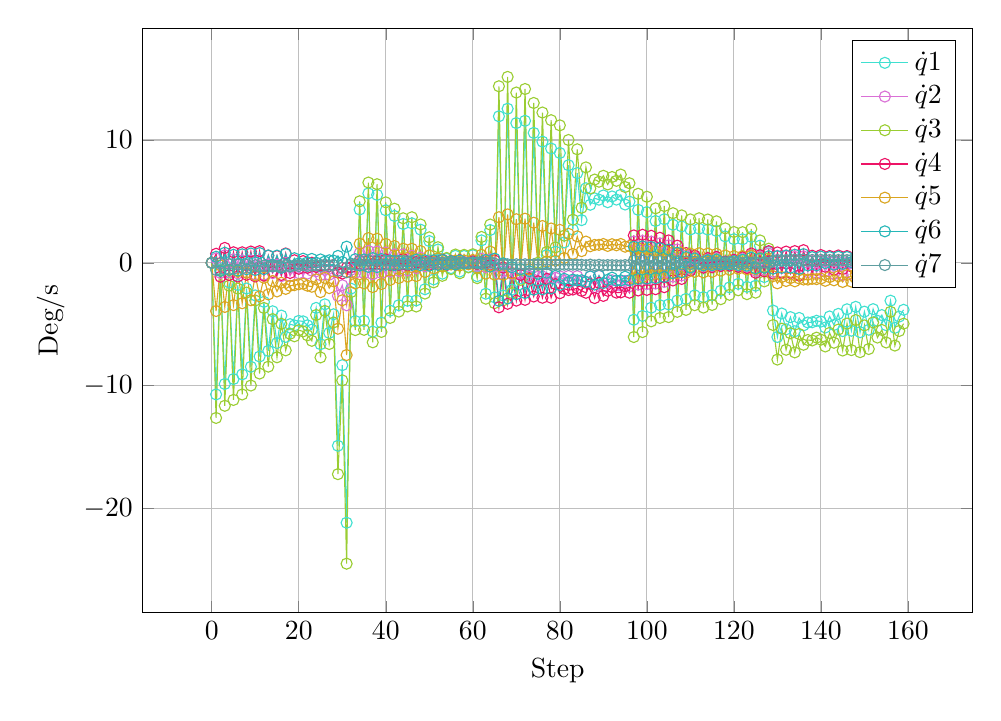
\begin{tikzpicture}
		\begin{axis}[height=9cm, width=\textwidth, grid=major,
		xlabel={Step},ylabel={Deg/s}
		]
			\addplot [color=Turquoise, mark=o] coordinates {
				(0, 0.000)
				(1, -10.720)
				(2, -0.541)
				(3, -9.868)
				(4, -1.603)
				(5, -9.466)
				(6, -1.813)
				(7, -9.086)
				(8, -2.094)
				(9, -8.465)
				(10, -2.656)
				(11, -7.633)
				(12, -3.180)
				(13, -7.172)
				(14, -3.948)
				(15, -6.529)
				(16, -4.299)
				(17, -6.032)
				(18, -4.998)
				(19, -5.097)
				(20, -4.730)
				(21, -4.769)
				(22, -5.091)
				(23, -5.442)
				(24, -3.672)
				(25, -6.631)
				(26, -3.382)
				(27, -5.710)
				(28, -4.194)
				(29, -14.900)
				(30, -8.337)
				(31, -21.170)
				(32, -2.103)
				(33, -4.742)
				(34, 4.342)
				(35, -4.728)
				(36, 5.656)
				(37, -5.599)
				(38, 5.534)
				(39, -4.872)
				(40, 4.280)
				(41, -3.896)
				(42, 3.816)
				(43, -3.451)
				(44, 3.165)
				(45, -3.090)
				(46, 3.217)
				(47, -3.065)
				(48, 2.699)
				(49, -2.153)
				(50, 1.770)
				(51, -1.355)
				(52, 1.082)
				(53, -0.885)
				(54, 0.319)
				(55, -0.428)
				(56, 0.565)
				(57, -0.710)
				(58, 0.558)
				(59, -0.330)
				(60, 0.619)
				(61, -1.091)
				(62, 1.828)
				(63, -2.518)
				(64, 2.669)
				(65, -2.814)
				(66, 11.933)
				(67, -2.669)
				(68, 12.550)
				(69, -2.186)
				(70, 11.383)
				(71, -1.266)
				(72, 11.567)
				(73, -1.190)
				(74, 10.582)
				(75, -0.113)
				(76, 9.871)
				(77, 0.628)
				(78, 9.309)
				(79, 0.907)
				(80, 8.945)
				(81, 1.663)
				(82, 7.949)
				(83, 2.709)
				(84, 7.308)
				(85, 3.475)
				(86, 6.071)
				(87, 4.730)
				(88, 5.253)
				(89, 5.145)
				(90, 5.487)
				(91, 4.937)
				(92, 5.405)
				(93, 5.150)
				(94, 5.537)
				(95, 4.749)
				(96, 4.980)
				(97, -4.635)
				(98, 4.314)
				(99, -4.326)
				(100, 4.131)
				(101, -3.657)
				(102, 3.405)
				(103, -3.447)
				(104, 3.550)
				(105, -3.391)
				(106, 3.102)
				(107, -3.064)
				(108, 2.964)
				(109, -2.940)
				(110, 2.711)
				(111, -2.647)
				(112, 2.783)
				(113, -2.797)
				(114, 2.704)
				(115, -2.632)
				(116, 2.592)
				(117, -2.271)
				(118, 2.152)
				(119, -1.997)
				(120, 1.926)
				(121, -1.713)
				(122, 1.914)
				(123, -1.958)
				(124, 2.113)
				(125, -1.862)
				(126, 1.399)
				(127, -1.159)
				(128, 0.883)
				(129, -3.888)
				(130, -6.039)
				(131, -4.129)
				(132, -5.418)
				(133, -4.424)
				(134, -5.577)
				(135, -4.488)
				(136, -5.094)
				(137, -4.862)
				(138, -4.840)
				(139, -4.722)
				(140, -4.788)
				(141, -5.270)
				(142, -4.370)
				(143, -5.062)
				(144, -4.159)
				(145, -5.561)
				(146, -3.786)
				(147, -5.530)
				(148, -3.586)
				(149, -5.648)
				(150, -3.978)
				(151, -5.450)
				(152, -3.774)
				(153, -4.721)
				(154, -4.258)
				(155, -5.080)
				(156, -3.085)
				(157, -5.295)
				(158, -4.379)
				(159, -3.828)
			};
			\addlegendentry{$\dot q$1}

			\addplot [color=Orchid, mark=o] coordinates {
				(0, 0.000)
				(1, 0.355)
				(2, -0.821)
				(3, 0.613)
				(4, -0.761)
				(5, 0.274)
				(6, -0.868)
				(7, 0.191)
				(8, -0.796)
				(9, 0.184)
				(10, -0.950)
				(11, 0.180)
				(12, -0.965)
				(13, -0.118)
				(14, -0.842)
				(15, -0.152)
				(16, -1.083)
				(17, -0.014)
				(18, -1.081)
				(19, -0.369)
				(20, -0.849)
				(21, -0.425)
				(22, -0.875)
				(23, -0.641)
				(24, -0.690)
				(25, -1.007)
				(26, -0.575)
				(27, -0.972)
				(28, -0.703)
				(29, -2.687)
				(30, -1.825)
				(31, -3.455)
				(32, -0.578)
				(33, -0.813)
				(34, 0.790)
				(35, -0.841)
				(36, 0.970)
				(37, -0.926)
				(38, 0.920)
				(39, -0.833)
				(40, 0.841)
				(41, -0.726)
				(42, 0.688)
				(43, -0.659)
				(44, 0.696)
				(45, -0.620)
				(46, 0.575)
				(47, -0.438)
				(48, 0.426)
				(49, -0.283)
				(50, 0.152)
				(51, -0.089)
				(52, 0.070)
				(53, 0.046)
				(54, -0.081)
				(55, 0.043)
				(56, -0.017)
				(57, 0.048)
				(58, 0.074)
				(59, -0.100)
				(60, 0.176)
				(61, -0.236)
				(62, 0.337)
				(63, -0.353)
				(64, 0.288)
				(65, -0.293)
				(66, -0.876)
				(67, -0.679)
				(68, -0.664)
				(69, -0.918)
				(70, -0.832)
				(71, -0.885)
				(72, -0.859)
				(73, -1.074)
				(74, -0.864)
				(75, -1.125)
				(76, -1.107)
				(77, -0.909)
				(78, -1.256)
				(79, -1.217)
				(80, -1.101)
				(81, -1.452)
				(82, -1.074)
				(83, -1.452)
				(84, -1.085)
				(85, -1.539)
				(86, -1.542)
				(87, -1.098)
				(88, -1.988)
				(89, -1.062)
				(90, -1.912)
				(91, -1.634)
				(92, -1.427)
				(93, -1.816)
				(94, -1.831)
				(95, -1.480)
				(96, -1.924)
				(97, 1.732)
				(98, -1.774)
				(99, 1.776)
				(100, -1.735)
				(101, 1.717)
				(102, -1.691)
				(103, 1.588)
				(104, -1.560)
				(105, 1.423)
				(106, -1.127)
				(107, 1.086)
				(108, -1.029)
				(109, 0.609)
				(110, -0.485)
				(111, 0.441)
				(112, -0.039)
				(113, -0.331)
				(114, 0.319)
				(115, -0.302)
				(116, 0.397)
				(117, -0.224)
				(118, 0.086)
				(119, -0.198)
				(120, 0.207)
				(121, -0.271)
				(122, 0.368)
				(123, -0.348)
				(124, 0.610)
				(125, -0.652)
				(126, 0.497)
				(127, -0.555)
				(128, 0.754)
				(129, -0.731)
				(130, 0.576)
				(131, -0.746)
				(132, 0.554)
				(133, -0.831)
				(134, 0.491)
				(135, -1.045)
				(136, 0.519)
				(137, -0.765)
				(138, 0.125)
				(139, -0.820)
				(140, 0.121)
				(141, -0.701)
				(142, 0.046)
				(143, -0.921)
				(144, 0.057)
				(145, -0.989)
				(146, 0.020)
				(147, -0.873)
				(148, -0.139)
				(149, -0.731)
				(150, -0.687)
				(151, -0.681)
				(152, -0.506)
				(153, -0.525)
				(154, -0.591)
				(155, -0.884)
				(156, -0.252)
				(157, -0.998)
				(158, -0.941)
				(159, -0.281)
			};
			\addlegendentry{$\dot q$2}

			\addplot [color=YellowGreen, mark=o] coordinates {
				(0, 0.000)
				(1, -12.636)
				(2, -0.624)
				(3, -11.645)
				(4, -1.867)
				(5, -11.168)
				(6, -2.101)
				(7, -10.723)
				(8, -2.426)
				(9, -9.995)
				(10, -3.070)
				(11, -9.020)
				(12, -3.677)
				(13, -8.457)
				(14, -4.585)
				(15, -7.697)
				(16, -4.968)
				(17, -7.128)
				(18, -5.784)
				(19, -5.985)
				(20, -5.489)
				(21, -5.588)
				(22, -5.906)
				(23, -6.352)
				(24, -4.248)
				(25, -7.704)
				(26, -3.918)
				(27, -6.612)
				(28, -4.856)
				(29, -17.213)
				(30, -9.572)
				(31, -24.505)
				(32, -2.390)
				(33, -5.479)
				(34, 5.010)
				(35, -5.457)
				(36, 6.538)
				(37, -6.475)
				(38, 6.402)
				(39, -5.629)
				(40, 4.925)
				(41, -4.489)
				(42, 4.404)
				(43, -3.974)
				(44, 3.627)
				(45, -3.552)
				(46, 3.713)
				(47, -3.557)
				(48, 3.126)
				(49, -2.504)
				(50, 2.074)
				(51, -1.593)
				(52, 1.272)
				(53, -1.061)
				(54, 0.395)
				(55, -0.516)
				(56, 0.675)
				(57, -0.853)
				(58, 0.649)
				(59, -0.372)
				(60, 0.701)
				(61, -1.251)
				(62, 2.106)
				(63, -2.922)
				(64, 3.116)
				(65, -3.286)
				(66, 14.380)
				(67, -3.060)
				(68, 15.143)
				(69, -2.462)
				(70, 13.869)
				(71, -1.391)
				(72, 14.157)
				(73, -1.289)
				(74, 13.020)
				(75, 0.014)
				(76, 12.241)
				(77, 0.885)
				(78, 11.616)
				(79, 1.257)
				(80, 11.197)
				(81, 2.212)
				(82, 10.004)
				(83, 3.512)
				(84, 9.244)
				(85, 4.486)
				(86, 7.772)
				(87, 6.057)
				(88, 6.779)
				(89, 6.607)
				(90, 7.088)
				(91, 6.385)
				(92, 6.989)
				(93, 6.678)
				(94, 7.188)
				(95, 6.173)
				(96, 6.483)
				(97, -6.044)
				(98, 5.622)
				(99, -5.641)
				(100, 5.383)
				(101, -4.768)
				(102, 4.436)
				(103, -4.494)
				(104, 4.626)
				(105, -4.422)
				(106, 4.042)
				(107, -3.994)
				(108, 3.863)
				(109, -3.835)
				(110, 3.535)
				(111, -3.451)
				(112, 3.628)
				(113, -3.648)
				(114, 3.526)
				(115, -3.433)
				(116, 3.381)
				(117, -2.961)
				(118, 2.807)
				(119, -2.605)
				(120, 2.513)
				(121, -2.234)
				(122, 2.497)
				(123, -2.553)
				(124, 2.756)
				(125, -2.429)
				(126, 1.825)
				(127, -1.512)
				(128, 1.152)
				(129, -5.068)
				(130, -7.880)
				(131, -5.367)
				(132, -7.080)
				(133, -5.735)
				(134, -7.296)
				(135, -5.796)
				(136, -6.675)
				(137, -6.288)
				(138, -6.323)
				(139, -6.095)
				(140, -6.259)
				(141, -6.812)
				(142, -5.707)
				(143, -6.510)
				(144, -5.436)
				(145, -7.145)
				(146, -4.947)
				(147, -7.110)
				(148, -4.667)
				(149, -7.276)
				(150, -5.098)
				(151, -7.020)
				(152, -4.854)
				(153, -6.086)
				(154, -5.467)
				(155, -6.487)
				(156, -3.991)
				(157, -6.740)
				(158, -5.549)
				(159, -4.958)
			};
			\addlegendentry{$\dot q$3}

			\addplot [color=WildStrawberry, mark=o] coordinates {
				(0, 0.000)
				(1, 0.735)
				(2, -1.133)
				(3, 1.213)
				(4, -1.001)
				(5, 0.858)
				(6, -1.115)
				(7, 0.853)
				(8, -0.970)
				(9, 0.918)
				(10, -1.109)
				(11, 0.948)
				(12, -1.044)
				(13, 0.585)
				(14, -0.743)
				(15, 0.552)
				(16, -0.984)
				(17, 0.762)
				(18, -0.829)
				(19, 0.208)
				(20, -0.486)
				(21, 0.139)
				(22, -0.408)
				(23, 0.006)
				(24, -0.338)
				(25, -0.228)
				(26, -0.189)
				(27, -0.284)
				(28, -0.176)
				(29, -0.793)
				(30, -0.869)
				(31, -0.416)
				(32, -0.363)
				(33, -0.115)
				(34, 0.190)
				(35, -0.155)
				(36, 0.169)
				(37, -0.085)
				(38, 0.124)
				(39, -0.115)
				(40, 0.273)
				(41, -0.177)
				(42, 0.157)
				(43, -0.180)
				(44, 0.303)
				(45, -0.203)
				(46, 0.124)
				(47, 0.044)
				(48, 0.025)
				(49, 0.065)
				(50, -0.161)
				(51, 0.164)
				(52, -0.132)
				(53, 0.252)
				(54, -0.181)
				(55, 0.151)
				(56, -0.143)
				(57, 0.218)
				(58, -0.016)
				(59, -0.070)
				(60, 0.113)
				(61, -0.095)
				(62, 0.083)
				(63, 0.048)
				(64, -0.163)
				(65, 0.195)
				(66, -3.627)
				(67, -0.391)
				(68, -3.337)
				(69, -0.836)
				(70, -3.079)
				(71, -0.992)
				(72, -3.015)
				(73, -1.268)
				(74, -2.744)
				(75, -1.503)
				(76, -2.845)
				(77, -1.306)
				(78, -2.847)
				(79, -1.736)
				(80, -2.476)
				(81, -2.110)
				(82, -2.221)
				(83, -2.177)
				(84, -2.067)
				(85, -2.283)
				(86, -2.439)
				(87, -1.731)
				(88, -2.872)
				(89, -1.631)
				(90, -2.694)
				(91, -2.274)
				(92, -1.981)
				(93, -2.429)
				(94, -2.408)
				(95, -1.913)
				(96, -2.434)
				(97, 2.231)
				(98, -2.253)
				(99, 2.284)
				(100, -2.205)
				(101, 2.201)
				(102, -2.148)
				(103, 2.037)
				(104, -1.983)
				(105, 1.826)
				(106, -1.435)
				(107, 1.397)
				(108, -1.312)
				(109, 0.793)
				(110, -0.624)
				(111, 0.578)
				(112, -0.062)
				(113, -0.395)
				(114, 0.391)
				(115, -0.360)
				(116, 0.489)
				(117, -0.266)
				(118, 0.098)
				(119, -0.235)
				(120, 0.252)
				(121, -0.330)
				(122, 0.455)
				(123, -0.424)
				(124, 0.760)
				(125, -0.810)
				(126, 0.620)
				(127, -0.692)
				(128, 0.947)
				(129, -0.879)
				(130, 0.847)
				(131, -0.811)
				(132, 0.914)
				(133, -0.819)
				(134, 0.954)
				(135, -1.022)
				(136, 1.030)
				(137, -0.576)
				(138, 0.580)
				(139, -0.594)
				(140, 0.633)
				(141, -0.320)
				(142, 0.554)
				(143, -0.558)
				(144, 0.597)
				(145, -0.512)
				(146, 0.550)
				(147, -0.302)
				(148, 0.364)
				(149, -0.039)
				(150, -0.227)
				(151, 0.092)
				(152, 0.038)
				(153, 0.211)
				(154, 0.062)
				(155, -0.125)
				(156, 0.300)
				(157, -0.178)
				(158, -0.273)
				(159, 0.473)
			};
			\addlegendentry{$\dot q$4}

			\addplot [color=Goldenrod, mark=o] coordinates {
				(0, 0.000)
				(1, -3.924)
				(2, -0.214)
				(3, -3.594)
				(4, -0.610)
				(5, -3.443)
				(6, -0.697)
				(7, -3.291)
				(8, -0.803)
				(9, -3.050)
				(10, -1.021)
				(11, -2.732)
				(12, -1.216)
				(13, -2.572)
				(14, -1.481)
				(15, -2.331)
				(16, -1.627)
				(17, -2.124)
				(18, -1.871)
				(19, -1.820)
				(20, -1.745)
				(21, -1.701)
				(22, -1.865)
				(23, -1.948)
				(24, -1.347)
				(25, -2.389)
				(26, -1.225)
				(27, -2.061)
				(28, -1.508)
				(29, -5.367)
				(30, -3.051)
				(31, -7.512)
				(32, -0.787)
				(33, -1.680)
				(34, 1.551)
				(35, -1.680)
				(36, 2.010)
				(37, -1.977)
				(38, 1.962)
				(39, -1.726)
				(40, 1.541)
				(41, -1.392)
				(42, 1.363)
				(43, -1.236)
				(44, 1.153)
				(45, -1.113)
				(46, 1.148)
				(47, -1.072)
				(48, 0.953)
				(49, -0.749)
				(50, 0.601)
				(51, -0.455)
				(52, 0.363)
				(53, -0.278)
				(54, 0.088)
				(55, -0.131)
				(56, 0.180)
				(57, -0.221)
				(58, 0.194)
				(59, -0.125)
				(60, 0.233)
				(61, -0.397)
				(62, 0.655)
				(63, -0.880)
				(64, 0.918)
				(65, -0.965)
				(66, 3.714)
				(67, -0.979)
				(68, 3.943)
				(69, -0.852)
				(70, 3.548)
				(71, -0.530)
				(72, 3.594)
				(73, -0.518)
				(74, 3.265)
				(75, -0.169)
				(76, 2.998)
				(77, 0.100)
				(78, 2.796)
				(79, 0.165)
				(80, 2.685)
				(81, 0.390)
				(82, 2.364)
				(83, 0.721)
				(84, 2.155)
				(85, 0.951)
				(86, 1.728)
				(87, 1.350)
				(88, 1.459)
				(89, 1.465)
				(90, 1.530)
				(91, 1.376)
				(92, 1.513)
				(93, 1.428)
				(94, 1.533)
				(95, 1.312)
				(96, 1.369)
				(97, -1.278)
				(98, 1.187)
				(99, -1.191)
				(100, 1.136)
				(101, -1.006)
				(102, 0.935)
				(103, -0.948)
				(104, 0.976)
				(105, -0.934)
				(106, 0.855)
				(107, -0.845)
				(108, 0.817)
				(109, -0.813)
				(110, 0.750)
				(111, -0.733)
				(112, 0.774)
				(113, -0.779)
				(114, 0.753)
				(115, -0.733)
				(116, 0.723)
				(117, -0.633)
				(118, 0.599)
				(119, -0.556)
				(120, 0.537)
				(121, -0.478)
				(122, 0.534)
				(123, -0.546)
				(124, 0.592)
				(125, -0.522)
				(126, 0.392)
				(127, -0.326)
				(128, 0.250)
				(129, -1.087)
				(130, -1.671)
				(131, -1.157)
				(132, -1.481)
				(133, -1.243)
				(134, -1.507)
				(135, -1.273)
				(136, -1.361)
				(137, -1.364)
				(138, -1.304)
				(139, -1.328)
				(140, -1.280)
				(141, -1.466)
				(142, -1.164)
				(143, -1.424)
				(144, -1.097)
				(145, -1.558)
				(146, -0.992)
				(147, -1.533)
				(148, -0.947)
				(149, -1.541)
				(150, -1.102)
				(151, -1.470)
				(152, -1.019)
				(153, -1.256)
				(154, -1.145)
				(155, -1.385)
				(156, -0.798)
				(157, -1.447)
				(158, -1.209)
				(159, -0.968)
			};
			\addlegendentry{$\dot q$5}

			\addplot [color=BlueGreen, mark=o] coordinates {
				(0, 0.000)
				(1, 0.495)
				(2, -0.667)
				(3, 0.822)
				(4, -0.573)
				(5, 0.655)
				(6, -0.630)
				(7, 0.692)
				(8, -0.529)
				(9, 0.760)
				(10, -0.587)
				(11, 0.794)
				(12, -0.520)
				(13, 0.599)
				(14, -0.297)
				(15, 0.589)
				(16, -0.410)
				(17, 0.723)
				(18, -0.265)
				(19, 0.374)
				(20, -0.051)
				(21, 0.337)
				(22, 0.035)
				(23, 0.317)
				(24, 0.014)
				(25, 0.273)
				(26, 0.101)
				(27, 0.205)
				(28, 0.179)
				(29, 0.564)
				(30, 0.067)
				(31, 1.316)
				(32, -0.064)
				(33, 0.295)
				(34, -0.215)
				(35, 0.271)
				(36, -0.329)
				(37, 0.381)
				(38, -0.347)
				(39, 0.306)
				(40, -0.161)
				(41, 0.192)
				(42, -0.196)
				(43, 0.156)
				(44, -0.057)
				(45, 0.114)
				(46, -0.171)
				(47, 0.264)
				(48, -0.192)
				(49, 0.206)
				(50, -0.235)
				(51, 0.206)
				(52, -0.164)
				(53, 0.223)
				(54, -0.136)
				(55, 0.126)
				(56, -0.132)
				(57, 0.189)
				(58, -0.053)
				(59, -0.017)
				(60, 0.022)
				(61, 0.026)
				(62, -0.090)
				(63, 0.225)
				(64, -0.306)
				(65, 0.339)
				(66, -3.100)
				(67, -0.044)
				(68, -2.901)
				(69, -0.359)
				(70, -2.552)
				(71, -0.521)
				(72, -2.462)
				(73, -0.694)
				(74, -2.190)
				(75, -0.890)
				(76, -2.161)
				(77, -0.804)
				(78, -2.086)
				(79, -1.063)
				(80, -1.806)
				(81, -1.302)
				(82, -1.578)
				(83, -1.363)
				(84, -1.430)
				(85, -1.422)
				(86, -1.566)
				(87, -1.111)
				(88, -1.770)
				(89, -1.039)
				(90, -1.646)
				(91, -1.384)
				(92, -1.209)
				(93, -1.453)
				(94, -1.433)
				(95, -1.132)
				(96, -1.423)
				(97, 1.308)
				(98, -1.315)
				(99, 1.337)
				(100, -1.287)
				(101, 1.285)
				(102, -1.250)
				(103, 1.190)
				(104, -1.156)
				(105, 1.068)
				(106, -0.840)
				(107, 0.820)
				(108, -0.769)
				(109, 0.472)
				(110, -0.373)
				(111, 0.347)
				(112, -0.051)
				(113, -0.210)
				(114, 0.209)
				(115, -0.191)
				(116, 0.266)
				(117, -0.139)
				(118, 0.044)
				(119, -0.123)
				(120, 0.134)
				(121, -0.179)
				(122, 0.250)
				(123, -0.232)
				(124, 0.424)
				(125, -0.453)
				(126, 0.348)
				(127, -0.390)
				(128, 0.538)
				(129, -0.479)
				(130, 0.538)
				(131, -0.416)
				(132, 0.600)
				(133, -0.395)
				(134, 0.655)
				(135, -0.495)
				(136, 0.708)
				(137, -0.214)
				(138, 0.461)
				(139, -0.212)
				(140, 0.507)
				(141, -0.020)
				(142, 0.465)
				(143, -0.149)
				(144, 0.498)
				(145, -0.086)
				(146, 0.471)
				(147, 0.053)
				(148, 0.367)
				(149, 0.230)
				(150, 0.051)
				(151, 0.325)
				(152, 0.216)
				(153, 0.374)
				(154, 0.268)
				(155, 0.211)
				(156, 0.355)
				(157, 0.206)
				(158, 0.102)
				(159, 0.521)
			};
			\addlegendentry{$\dot q$6}

			\addplot [color=CadetBlue, mark=o] coordinates {
				(0, 0.000)
				(1, -0.585)
				(2, -0.047)
				(3, -0.518)
				(4, -0.113)
				(5, -0.490)
				(6, -0.137)
				(7, -0.452)
				(8, -0.155)
				(9, -0.401)
				(10, -0.199)
				(11, -0.339)
				(12, -0.230)
				(13, -0.321)
				(14, -0.251)
				(15, -0.278)
				(16, -0.289)
				(17, -0.220)
				(18, -0.310)
				(19, -0.213)
				(20, -0.261)
				(21, -0.195)
				(22, -0.264)
				(23, -0.228)
				(24, -0.191)
				(25, -0.292)
				(26, -0.156)
				(27, -0.253)
				(28, -0.178)
				(29, -0.639)
				(30, -0.412)
				(31, -0.766)
				(32, -0.123)
				(33, -0.166)
				(34, 0.168)
				(35, -0.172)
				(36, 0.207)
				(37, -0.189)
				(38, 0.197)
				(39, -0.171)
				(40, 0.179)
				(41, -0.150)
				(42, 0.147)
				(43, -0.137)
				(44, 0.148)
				(45, -0.129)
				(46, 0.122)
				(47, -0.091)
				(48, 0.091)
				(49, -0.059)
				(50, 0.032)
				(51, -0.018)
				(52, 0.015)
				(53, 0.010)
				(54, -0.017)
				(55, 0.009)
				(56, -0.004)
				(57, 0.011)
				(58, 0.016)
				(59, -0.021)
				(60, 0.037)
				(61, -0.050)
				(62, 0.072)
				(63, -0.074)
				(64, 0.062)
				(65, -0.061)
				(66, -0.172)
				(67, -0.135)
				(68, -0.120)
				(69, -0.172)
				(70, -0.120)
				(71, -0.145)
				(72, -0.120)
				(73, -0.161)
				(74, -0.124)
				(75, -0.155)
				(76, -0.160)
				(77, -0.115)
				(78, -0.177)
				(79, -0.141)
				(80, -0.162)
				(81, -0.156)
				(82, -0.161)
				(83, -0.151)
				(84, -0.163)
				(85, -0.159)
				(86, -0.199)
				(87, -0.148)
				(88, -0.208)
				(89, -0.161)
				(90, -0.207)
				(91, -0.185)
				(92, -0.193)
				(93, -0.198)
				(94, -0.214)
				(95, -0.185)
				(96, -0.200)
				(97, 0.179)
				(98, -0.171)
				(99, 0.168)
				(100, -0.164)
				(101, 0.143)
				(102, -0.136)
				(103, 0.135)
				(104, -0.141)
				(105, 0.132)
				(106, -0.121)
				(107, 0.118)
				(108, -0.116)
				(109, 0.113)
				(110, -0.104)
				(111, 0.101)
				(112, -0.104)
				(113, 0.104)
				(114, -0.100)
				(115, 0.098)
				(116, -0.095)
				(117, 0.084)
				(118, -0.080)
				(119, 0.074)
				(120, -0.072)
				(121, 0.064)
				(122, -0.070)
				(123, 0.072)
				(124, -0.076)
				(125, 0.067)
				(126, -0.050)
				(127, 0.041)
				(128, -0.030)
				(129, 0.142)
				(130, 0.234)
				(131, 0.146)
				(132, 0.231)
				(133, 0.154)
				(134, 0.260)
				(135, 0.143)
				(136, 0.256)
				(137, 0.173)
				(138, 0.234)
				(139, 0.164)
				(140, 0.244)
				(141, 0.205)
				(142, 0.229)
				(143, 0.179)
				(144, 0.233)
				(145, 0.206)
				(146, 0.221)
				(147, 0.226)
				(148, 0.203)
				(149, 0.262)
				(150, 0.166)
				(151, 0.277)
				(152, 0.191)
				(153, 0.263)
				(154, 0.224)
				(155, 0.246)
				(156, 0.201)
				(157, 0.255)
				(158, 0.198)
				(159, 0.278)
			};
			\addlegendentry{$\dot q$7}

			\addplot[Turquoise,sharp plot,update limits=false] coordinates {
				(0,90)
				(159,90)
			};
			\addplot[Turquoise,sharp plot,update limits=false] coordinates {
				(0,-90)
				(159,-90)
			};

			\addplot[Orchid,sharp plot,update limits=false] coordinates {
				(0,94)
				(159,94)
			};
			\addplot[Orchid,sharp plot,update limits=false] coordinates {
				(0,-94)
				(159,-94)
			};

			\addplot[YellowGreen,sharp plot,update limits=false] coordinates {
				(0,180)
				(159,180)
			};
			\addplot[YellowGreen,sharp plot,update limits=false] coordinates {
				(0,-180)
				(159,-180)
			};

			\addplot[WildStrawberry,sharp plot,update limits=false] coordinates {
				(0,143)
				(159,143)
			};
			\addplot[WildStrawberry,sharp plot,update limits=false] coordinates {
				(0,-143)
				(159,-143)
			};

			\addplot[Goldenrod,sharp plot,update limits=false] coordinates {
				(0,270)
				(159,270)
			};
			\addplot[Goldenrod,sharp plot,update limits=false] coordinates {
				(0,-270)
				(159,-270)
			};

			\addplot[BlueGreen,sharp plot,update limits=false] coordinates {
				(0,120)
				(159,120)
			};
			\addplot[BlueGreen,sharp plot,update limits=false] coordinates {
				(0,-120)
				(159,-120)
			};

			\addplot[CadetBlue,sharp plot,update limits=false] coordinates {
				(0,360)
				(159,360)
			};
			\addplot[CadetBlue,sharp plot,update limits=false] coordinates {
				(0,-360)
				(159,-360)
			};
		\end{axis}
	\end{tikzpicture}
	\caption{Robot joint's speed while tracking the dots marker at medium speed.}
	\label{fig:speedColorMediumPlot}
\end{figure}
}

\providecommand{\cameraPoseColorMediumPlot}{
\begin{figure}[!ht]
	\centering
	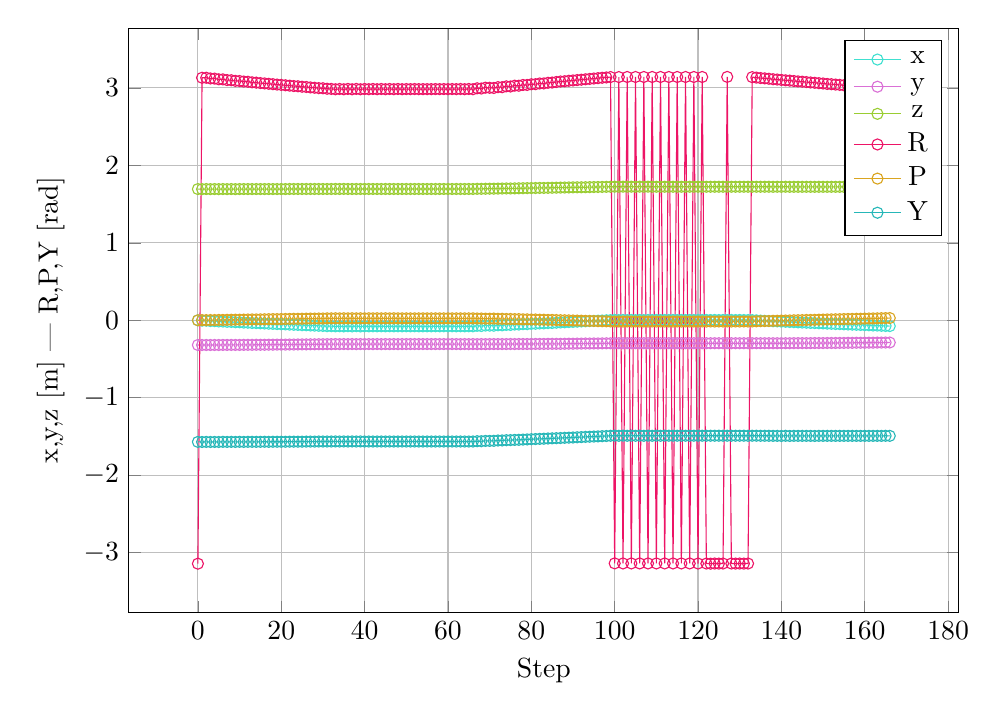
\begin{tikzpicture}
		\begin{axis}[height=9cm, width=\textwidth, grid=major,
		xlabel={Step},ylabel={x,y,z [m] | R,P,Y [rad]}
		]
			\addplot [color=Turquoise, mark=o] coordinates {
				(0, 0.000)
				(1, -0.005)
				(2, -0.005)
				(3, -0.010)
				(4, -0.011)
				(5, -0.015)
				(6, -0.016)
				(7, -0.020)
				(8, -0.021)
				(9, -0.025)
				(10, -0.026)
				(11, -0.030)
				(12, -0.031)
				(13, -0.035)
				(14, -0.036)
				(15, -0.039)
				(16, -0.041)
				(17, -0.044)
				(18, -0.046)
				(19, -0.049)
				(20, -0.051)
				(21, -0.053)
				(22, -0.056)
				(23, -0.058)
				(24, -0.060)
				(25, -0.063)
				(26, -0.064)
				(27, -0.067)
				(28, -0.069)
				(29, -0.071)
				(30, -0.073)
				(31, -0.076)
				(32, -0.076)
				(33, -0.078)
				(34, -0.077)
				(35, -0.079)
				(36, -0.076)
				(37, -0.079)
				(38, -0.076)
				(39, -0.079)
				(40, -0.077)
				(41, -0.078)
				(42, -0.077)
				(43, -0.078)
				(44, -0.077)
				(45, -0.078)
				(46, -0.077)
				(47, -0.078)
				(48, -0.077)
				(49, -0.078)
				(50, -0.077)
				(51, -0.078)
				(52, -0.077)
				(53, -0.078)
				(54, -0.078)
				(55, -0.078)
				(56, -0.078)
				(57, -0.077)
				(58, -0.078)
				(59, -0.077)
				(60, -0.077)
				(61, -0.077)
				(62, -0.078)
				(63, -0.077)
				(64, -0.078)
				(65, -0.077)
				(66, -0.078)
				(67, -0.072)
				(68, -0.074)
				(69, -0.068)
				(70, -0.069)
				(71, -0.070)
				(72, -0.064)
				(73, -0.065)
				(74, -0.060)
				(75, -0.060)
				(76, -0.055)
				(77, -0.055)
				(78, -0.050)
				(79, -0.050)
				(80, -0.046)
				(81, -0.045)
				(82, -0.041)
				(83, -0.040)
				(84, -0.036)
				(85, -0.035)
				(86, -0.031)
				(87, -0.028)
				(88, -0.026)
				(89, -0.023)
				(90, -0.021)
				(91, -0.018)
				(92, -0.015)
				(93, -0.013)
				(94, -0.010)
				(95, -0.008)
				(96, -0.005)
				(97, -0.003)
				(98, -0.000)
				(99, 0.002)
				(100, 0.005)
				(101, 0.002)
				(102, 0.004)
				(103, 0.002)
				(104, 0.004)
				(105, 0.002)
				(106, 0.004)
				(107, 0.002)
				(108, 0.004)
				(109, 0.003)
				(110, 0.004)
				(111, 0.003)
				(112, 0.004)
				(113, 0.003)
				(114, 0.004)
				(115, 0.003)
				(116, 0.004)
				(117, 0.003)
				(118, 0.004)
				(119, 0.003)
				(120, 0.004)
				(121, 0.003)
				(122, 0.004)
				(123, 0.003)
				(124, 0.004)
				(125, 0.003)
				(126, 0.004)
				(127, 0.003)
				(128, 0.004)
				(129, 0.003)
				(130, 0.004)
				(131, 0.003)
				(132, 0.003)
				(133, 0.002)
				(134, -0.001)
				(135, -0.004)
				(136, -0.007)
				(137, -0.009)
				(138, -0.012)
				(139, -0.014)
				(140, -0.017)
				(141, -0.019)
				(142, -0.022)
				(143, -0.024)
				(144, -0.027)
				(145, -0.029)
				(146, -0.031)
				(147, -0.034)
				(148, -0.036)
				(149, -0.038)
				(150, -0.040)
				(151, -0.043)
				(152, -0.045)
				(153, -0.048)
				(154, -0.049)
				(155, -0.052)
				(156, -0.054)
				(157, -0.056)
				(158, -0.058)
				(159, -0.060)
				(160, -0.062)
				(161, -0.064)
				(162, -0.067)
				(163, -0.068)
				(164, -0.071)
				(165, -0.073)
				(166, -0.075)
			};
			\addlegendentry{x}

			\addplot [color=Orchid, mark=o] coordinates {
				(0, -0.319)
				(1, -0.319)
				(2, -0.319)
				(3, -0.319)
				(4, -0.319)
				(5, -0.319)
				(6, -0.318)
				(7, -0.318)
				(8, -0.318)
				(9, -0.318)
				(10, -0.318)
				(11, -0.317)
				(12, -0.317)
				(13, -0.317)
				(14, -0.316)
				(15, -0.316)
				(16, -0.316)
				(17, -0.315)
				(18, -0.315)
				(19, -0.314)
				(20, -0.314)
				(21, -0.314)
				(22, -0.313)
				(23, -0.313)
				(24, -0.312)
				(25, -0.311)
				(26, -0.311)
				(27, -0.310)
				(28, -0.310)
				(29, -0.309)
				(30, -0.309)
				(31, -0.308)
				(32, -0.308)
				(33, -0.307)
				(34, -0.308)
				(35, -0.307)
				(36, -0.308)
				(37, -0.307)
				(38, -0.308)
				(39, -0.307)
				(40, -0.308)
				(41, -0.307)
				(42, -0.308)
				(43, -0.307)
				(44, -0.308)
				(45, -0.307)
				(46, -0.308)
				(47, -0.307)
				(48, -0.308)
				(49, -0.307)
				(50, -0.307)
				(51, -0.307)
				(52, -0.307)
				(53, -0.307)
				(54, -0.307)
				(55, -0.307)
				(56, -0.307)
				(57, -0.307)
				(58, -0.307)
				(59, -0.307)
				(60, -0.307)
				(61, -0.307)
				(62, -0.307)
				(63, -0.308)
				(64, -0.307)
				(65, -0.308)
				(66, -0.307)
				(67, -0.308)
				(68, -0.307)
				(69, -0.308)
				(70, -0.307)
				(71, -0.307)
				(72, -0.307)
				(73, -0.307)
				(74, -0.307)
				(75, -0.306)
				(76, -0.307)
				(77, -0.306)
				(78, -0.306)
				(79, -0.306)
				(80, -0.306)
				(81, -0.305)
				(82, -0.305)
				(83, -0.305)
				(84, -0.304)
				(85, -0.304)
				(86, -0.304)
				(87, -0.304)
				(88, -0.303)
				(89, -0.302)
				(90, -0.302)
				(91, -0.301)
				(92, -0.301)
				(93, -0.300)
				(94, -0.300)
				(95, -0.299)
				(96, -0.299)
				(97, -0.298)
				(98, -0.297)
				(99, -0.297)
				(100, -0.296)
				(101, -0.296)
				(102, -0.296)
				(103, -0.296)
				(104, -0.296)
				(105, -0.296)
				(106, -0.296)
				(107, -0.296)
				(108, -0.296)
				(109, -0.296)
				(110, -0.296)
				(111, -0.296)
				(112, -0.296)
				(113, -0.296)
				(114, -0.296)
				(115, -0.296)
				(116, -0.296)
				(117, -0.296)
				(118, -0.296)
				(119, -0.296)
				(120, -0.296)
				(121, -0.296)
				(122, -0.296)
				(123, -0.296)
				(124, -0.296)
				(125, -0.296)
				(126, -0.296)
				(127, -0.296)
				(128, -0.296)
				(129, -0.296)
				(130, -0.296)
				(131, -0.296)
				(132, -0.296)
				(133, -0.296)
				(134, -0.296)
				(135, -0.296)
				(136, -0.296)
				(137, -0.296)
				(138, -0.296)
				(139, -0.296)
				(140, -0.296)
				(141, -0.296)
				(142, -0.296)
				(143, -0.295)
				(144, -0.295)
				(145, -0.295)
				(146, -0.295)
				(147, -0.295)
				(148, -0.294)
				(149, -0.294)
				(150, -0.294)
				(151, -0.293)
				(152, -0.293)
				(153, -0.293)
				(154, -0.292)
				(155, -0.292)
				(156, -0.291)
				(157, -0.291)
				(158, -0.290)
				(159, -0.290)
				(160, -0.290)
				(161, -0.289)
				(162, -0.289)
				(163, -0.288)
				(164, -0.288)
				(165, -0.287)
				(166, -0.287)
			};
			\addlegendentry{y}

			\addplot [color=YellowGreen, mark=o] coordinates {
				(0, 1.694)
				(1, 1.693)
				(2, 1.694)
				(3, 1.693)
				(4, 1.694)
				(5, 1.693)
				(6, 1.694)
				(7, 1.693)
				(8, 1.694)
				(9, 1.693)
				(10, 1.694)
				(11, 1.694)
				(12, 1.694)
				(13, 1.694)
				(14, 1.694)
				(15, 1.694)
				(16, 1.694)
				(17, 1.694)
				(18, 1.694)
				(19, 1.694)
				(20, 1.694)
				(21, 1.694)
				(22, 1.695)
				(23, 1.695)
				(24, 1.695)
				(25, 1.695)
				(26, 1.695)
				(27, 1.695)
				(28, 1.695)
				(29, 1.695)
				(30, 1.695)
				(31, 1.695)
				(32, 1.695)
				(33, 1.696)
				(34, 1.695)
				(35, 1.696)
				(36, 1.695)
				(37, 1.695)
				(38, 1.695)
				(39, 1.695)
				(40, 1.695)
				(41, 1.695)
				(42, 1.695)
				(43, 1.695)
				(44, 1.695)
				(45, 1.695)
				(46, 1.695)
				(47, 1.695)
				(48, 1.695)
				(49, 1.695)
				(50, 1.695)
				(51, 1.695)
				(52, 1.695)
				(53, 1.695)
				(54, 1.695)
				(55, 1.695)
				(56, 1.695)
				(57, 1.695)
				(58, 1.695)
				(59, 1.695)
				(60, 1.695)
				(61, 1.695)
				(62, 1.695)
				(63, 1.695)
				(64, 1.695)
				(65, 1.695)
				(66, 1.695)
				(67, 1.697)
				(68, 1.697)
				(69, 1.698)
				(70, 1.699)
				(71, 1.699)
				(72, 1.700)
				(73, 1.701)
				(74, 1.702)
				(75, 1.702)
				(76, 1.703)
				(77, 1.704)
				(78, 1.705)
				(79, 1.706)
				(80, 1.707)
				(81, 1.708)
				(82, 1.709)
				(83, 1.709)
				(84, 1.710)
				(85, 1.711)
				(86, 1.712)
				(87, 1.713)
				(88, 1.714)
				(89, 1.715)
				(90, 1.716)
				(91, 1.717)
				(92, 1.717)
				(93, 1.718)
				(94, 1.719)
				(95, 1.720)
				(96, 1.721)
				(97, 1.722)
				(98, 1.723)
				(99, 1.724)
				(100, 1.725)
				(101, 1.724)
				(102, 1.725)
				(103, 1.724)
				(104, 1.725)
				(105, 1.724)
				(106, 1.725)
				(107, 1.724)
				(108, 1.725)
				(109, 1.724)
				(110, 1.724)
				(111, 1.724)
				(112, 1.724)
				(113, 1.724)
				(114, 1.724)
				(115, 1.724)
				(116, 1.724)
				(117, 1.724)
				(118, 1.724)
				(119, 1.724)
				(120, 1.724)
				(121, 1.724)
				(122, 1.724)
				(123, 1.724)
				(124, 1.724)
				(125, 1.724)
				(126, 1.724)
				(127, 1.724)
				(128, 1.724)
				(129, 1.724)
				(130, 1.724)
				(131, 1.724)
				(132, 1.724)
				(133, 1.724)
				(134, 1.724)
				(135, 1.724)
				(136, 1.724)
				(137, 1.724)
				(138, 1.723)
				(139, 1.724)
				(140, 1.723)
				(141, 1.724)
				(142, 1.723)
				(143, 1.723)
				(144, 1.723)
				(145, 1.723)
				(146, 1.723)
				(147, 1.723)
				(148, 1.723)
				(149, 1.723)
				(150, 1.723)
				(151, 1.723)
				(152, 1.723)
				(153, 1.723)
				(154, 1.723)
				(155, 1.723)
				(156, 1.723)
				(157, 1.723)
				(158, 1.723)
				(159, 1.723)
				(160, 1.723)
				(161, 1.723)
				(162, 1.723)
				(163, 1.723)
				(164, 1.723)
				(165, 1.723)
				(166, 1.723)
			};
			\addlegendentry{z}

			\addplot [color=WildStrawberry, mark=o] coordinates {
				(0, -3.142)
				(1, 3.131)
				(2, 3.131)
				(3, 3.122)
				(4, 3.120)
				(5, 3.111)
				(6, 3.110)
				(7, 3.101)
				(8, 3.099)
				(9, 3.091)
				(10, 3.089)
				(11, 3.082)
				(12, 3.079)
				(13, 3.072)
				(14, 3.068)
				(15, 3.062)
				(16, 3.058)
				(17, 3.053)
				(18, 3.048)
				(19, 3.043)
				(20, 3.039)
				(21, 3.034)
				(22, 3.029)
				(23, 3.024)
				(24, 3.021)
				(25, 3.015)
				(26, 3.012)
				(27, 3.006)
				(28, 3.002)
				(29, 2.997)
				(30, 2.995)
				(31, 2.989)
				(32, 2.987)
				(33, 2.982)
				(34, 2.986)
				(35, 2.982)
				(36, 2.987)
				(37, 2.982)
				(38, 2.987)
				(39, 2.982)
				(40, 2.986)
				(41, 2.983)
				(42, 2.986)
				(43, 2.983)
				(44, 2.986)
				(45, 2.983)
				(46, 2.986)
				(47, 2.983)
				(48, 2.986)
				(49, 2.983)
				(50, 2.985)
				(51, 2.984)
				(52, 2.985)
				(53, 2.984)
				(54, 2.984)
				(55, 2.984)
				(56, 2.984)
				(57, 2.985)
				(58, 2.984)
				(59, 2.985)
				(60, 2.984)
				(61, 2.985)
				(62, 2.984)
				(63, 2.986)
				(64, 2.983)
				(65, 2.986)
				(66, 2.983)
				(67, 2.995)
				(68, 2.992)
				(69, 3.003)
				(70, 3.001)
				(71, 2.999)
				(72, 3.010)
				(73, 3.009)
				(74, 3.020)
				(75, 3.018)
				(76, 3.029)
				(77, 3.028)
				(78, 3.038)
				(79, 3.038)
				(80, 3.047)
				(81, 3.048)
				(82, 3.057)
				(83, 3.058)
				(84, 3.066)
				(85, 3.069)
				(86, 3.076)
				(87, 3.083)
				(88, 3.086)
				(89, 3.092)
				(90, 3.096)
				(91, 3.101)
				(92, 3.106)
				(93, 3.111)
				(94, 3.116)
				(95, 3.121)
				(96, 3.126)
				(97, 3.131)
				(98, 3.135)
				(99, 3.140)
				(100, -3.138)
				(101, 3.140)
				(102, -3.139)
				(103, 3.141)
				(104, -3.139)
				(105, 3.141)
				(106, -3.139)
				(107, 3.141)
				(108, -3.139)
				(109, 3.141)
				(110, -3.139)
				(111, 3.141)
				(112, -3.139)
				(113, 3.141)
				(114, -3.139)
				(115, 3.141)
				(116, -3.139)
				(117, 3.141)
				(118, -3.139)
				(119, 3.141)
				(120, -3.140)
				(121, 3.141)
				(122, -3.140)
				(123, -3.142)
				(124, -3.140)
				(125, -3.141)
				(126, -3.140)
				(127, 3.142)
				(128, -3.140)
				(129, -3.141)
				(130, -3.140)
				(131, -3.141)
				(132, -3.140)
				(133, 3.139)
				(134, 3.133)
				(135, 3.127)
				(136, 3.123)
				(137, 3.118)
				(138, 3.112)
				(139, 3.108)
				(140, 3.103)
				(141, 3.098)
				(142, 3.094)
				(143, 3.089)
				(144, 3.084)
				(145, 3.080)
				(146, 3.075)
				(147, 3.070)
				(148, 3.066)
				(149, 3.061)
				(150, 3.057)
				(151, 3.051)
				(152, 3.048)
				(153, 3.043)
				(154, 3.039)
				(155, 3.034)
				(156, 3.030)
				(157, 3.027)
				(158, 3.021)
				(159, 3.018)
				(160, 3.013)
				(161, 3.009)
				(162, 3.005)
				(163, 3.002)
				(164, 2.997)
				(165, 2.993)
				(166, 2.989)
			};
			\addlegendentry{R}

			\addplot [color=Goldenrod, mark=o] coordinates {
				(0, -0.000)
				(1, 0.002)
				(2, 0.002)
				(3, 0.003)
				(4, 0.003)
				(5, 0.005)
				(6, 0.005)
				(7, 0.006)
				(8, 0.007)
				(9, 0.008)
				(10, 0.008)
				(11, 0.009)
				(12, 0.010)
				(13, 0.011)
				(14, 0.011)
				(15, 0.012)
				(16, 0.013)
				(17, 0.014)
				(18, 0.015)
				(19, 0.015)
				(20, 0.016)
				(21, 0.017)
				(22, 0.018)
				(23, 0.019)
				(24, 0.019)
				(25, 0.020)
				(26, 0.021)
				(27, 0.022)
				(28, 0.022)
				(29, 0.023)
				(30, 0.023)
				(31, 0.025)
				(32, 0.025)
				(33, 0.026)
				(34, 0.025)
				(35, 0.026)
				(36, 0.025)
				(37, 0.026)
				(38, 0.025)
				(39, 0.026)
				(40, 0.025)
				(41, 0.026)
				(42, 0.025)
				(43, 0.026)
				(44, 0.025)
				(45, 0.026)
				(46, 0.025)
				(47, 0.026)
				(48, 0.025)
				(49, 0.025)
				(50, 0.025)
				(51, 0.025)
				(52, 0.025)
				(53, 0.025)
				(54, 0.025)
				(55, 0.025)
				(56, 0.025)
				(57, 0.025)
				(58, 0.025)
				(59, 0.025)
				(60, 0.025)
				(61, 0.025)
				(62, 0.025)
				(63, 0.025)
				(64, 0.025)
				(65, 0.025)
				(66, 0.025)
				(67, 0.023)
				(68, 0.023)
				(69, 0.021)
				(70, 0.021)
				(71, 0.022)
				(72, 0.019)
				(73, 0.019)
				(74, 0.017)
				(75, 0.017)
				(76, 0.015)
				(77, 0.015)
				(78, 0.012)
				(79, 0.012)
				(80, 0.010)
				(81, 0.010)
				(82, 0.008)
				(83, 0.007)
				(84, 0.005)
				(85, 0.005)
				(86, 0.003)
				(87, 0.001)
				(88, 0.000)
				(89, -0.001)
				(90, -0.003)
				(91, -0.004)
				(92, -0.005)
				(93, -0.007)
				(94, -0.008)
				(95, -0.009)
				(96, -0.011)
				(97, -0.012)
				(98, -0.013)
				(99, -0.015)
				(100, -0.016)
				(101, -0.015)
				(102, -0.016)
				(103, -0.015)
				(104, -0.016)
				(105, -0.015)
				(106, -0.016)
				(107, -0.015)
				(108, -0.016)
				(109, -0.015)
				(110, -0.016)
				(111, -0.015)
				(112, -0.016)
				(113, -0.015)
				(114, -0.016)
				(115, -0.015)
				(116, -0.016)
				(117, -0.015)
				(118, -0.016)
				(119, -0.015)
				(120, -0.016)
				(121, -0.015)
				(122, -0.016)
				(123, -0.015)
				(124, -0.016)
				(125, -0.015)
				(126, -0.016)
				(127, -0.015)
				(128, -0.016)
				(129, -0.015)
				(130, -0.016)
				(131, -0.015)
				(132, -0.016)
				(133, -0.015)
				(134, -0.013)
				(135, -0.011)
				(136, -0.010)
				(137, -0.009)
				(138, -0.007)
				(139, -0.006)
				(140, -0.004)
				(141, -0.003)
				(142, -0.002)
				(143, -0.000)
				(144, 0.001)
				(145, 0.002)
				(146, 0.004)
				(147, 0.005)
				(148, 0.006)
				(149, 0.008)
				(150, 0.009)
				(151, 0.011)
				(152, 0.012)
				(153, 0.013)
				(154, 0.014)
				(155, 0.016)
				(156, 0.017)
				(157, 0.018)
				(158, 0.019)
				(159, 0.020)
				(160, 0.022)
				(161, 0.023)
				(162, 0.024)
				(163, 0.025)
				(164, 0.027)
				(165, 0.028)
				(166, 0.029)
			};
			\addlegendentry{P}

			\addplot [color=BlueGreen, mark=o] coordinates {
				(0, -1.570)
				(1, -1.571)
				(2, -1.570)
				(3, -1.571)
				(4, -1.570)
				(5, -1.571)
				(6, -1.569)
				(7, -1.570)
				(8, -1.569)
				(9, -1.570)
				(10, -1.569)
				(11, -1.570)
				(12, -1.569)
				(13, -1.569)
				(14, -1.569)
				(15, -1.569)
				(16, -1.568)
				(17, -1.569)
				(18, -1.568)
				(19, -1.568)
				(20, -1.568)
				(21, -1.568)
				(22, -1.567)
				(23, -1.567)
				(24, -1.567)
				(25, -1.567)
				(26, -1.566)
				(27, -1.566)
				(28, -1.566)
				(29, -1.565)
				(30, -1.565)
				(31, -1.565)
				(32, -1.565)
				(33, -1.564)
				(34, -1.565)
				(35, -1.564)
				(36, -1.565)
				(37, -1.564)
				(38, -1.565)
				(39, -1.564)
				(40, -1.565)
				(41, -1.565)
				(42, -1.565)
				(43, -1.565)
				(44, -1.565)
				(45, -1.565)
				(46, -1.565)
				(47, -1.565)
				(48, -1.565)
				(49, -1.565)
				(50, -1.565)
				(51, -1.565)
				(52, -1.565)
				(53, -1.565)
				(54, -1.565)
				(55, -1.565)
				(56, -1.565)
				(57, -1.565)
				(58, -1.565)
				(59, -1.565)
				(60, -1.565)
				(61, -1.565)
				(62, -1.565)
				(63, -1.565)
				(64, -1.565)
				(65, -1.565)
				(66, -1.565)
				(67, -1.561)
				(68, -1.561)
				(69, -1.557)
				(70, -1.557)
				(71, -1.556)
				(72, -1.552)
				(73, -1.551)
				(74, -1.548)
				(75, -1.547)
				(76, -1.544)
				(77, -1.543)
				(78, -1.540)
				(79, -1.538)
				(80, -1.535)
				(81, -1.533)
				(82, -1.531)
				(83, -1.529)
				(84, -1.526)
				(85, -1.524)
				(86, -1.522)
				(87, -1.520)
				(88, -1.517)
				(89, -1.515)
				(90, -1.513)
				(91, -1.510)
				(92, -1.508)
				(93, -1.505)
				(94, -1.503)
				(95, -1.501)
				(96, -1.499)
				(97, -1.496)
				(98, -1.494)
				(99, -1.491)
				(100, -1.489)
				(101, -1.491)
				(102, -1.489)
				(103, -1.491)
				(104, -1.489)
				(105, -1.491)
				(106, -1.489)
				(107, -1.491)
				(108, -1.489)
				(109, -1.491)
				(110, -1.489)
				(111, -1.491)
				(112, -1.489)
				(113, -1.490)
				(114, -1.490)
				(115, -1.490)
				(116, -1.490)
				(117, -1.490)
				(118, -1.490)
				(119, -1.490)
				(120, -1.490)
				(121, -1.490)
				(122, -1.490)
				(123, -1.490)
				(124, -1.490)
				(125, -1.490)
				(126, -1.490)
				(127, -1.490)
				(128, -1.490)
				(129, -1.490)
				(130, -1.490)
				(131, -1.490)
				(132, -1.491)
				(133, -1.490)
				(134, -1.490)
				(135, -1.491)
				(136, -1.491)
				(137, -1.491)
				(138, -1.492)
				(139, -1.492)
				(140, -1.493)
				(141, -1.491)
				(142, -1.493)
				(143, -1.492)
				(144, -1.492)
				(145, -1.492)
				(146, -1.492)
				(147, -1.492)
				(148, -1.493)
				(149, -1.492)
				(150, -1.492)
				(151, -1.492)
				(152, -1.492)
				(153, -1.492)
				(154, -1.492)
				(155, -1.492)
				(156, -1.492)
				(157, -1.492)
				(158, -1.492)
				(159, -1.492)
				(160, -1.492)
				(161, -1.492)
				(162, -1.492)
				(163, -1.492)
				(164, -1.492)
				(165, -1.491)
				(166, -1.492)
			};
			\addlegendentry{Y}

		\end{axis}
	\end{tikzpicture}
	\caption{Robot camera's frame while tracking the marker at medium speed.}
	\label{fig:cameraPoseColorMediumPlot}
\end{figure}
}

\providecommand{\errorColorPlot}{
\begin{figure}[!ht]
	\centering
	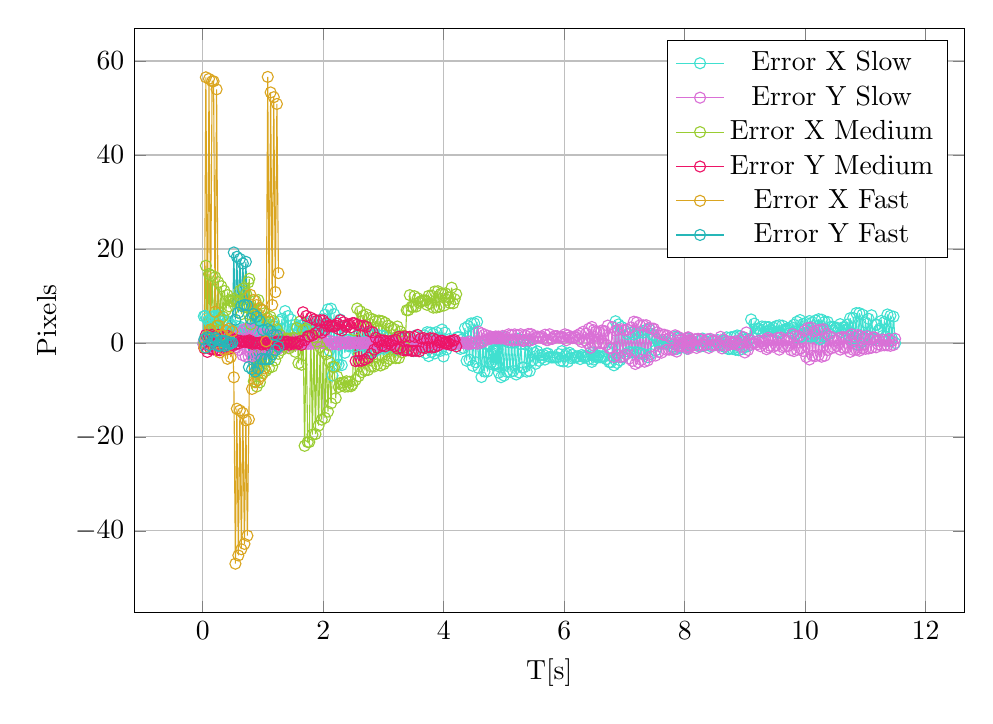
\begin{tikzpicture}
		\begin{axis}[height=9cm, width=\textwidth, grid=major,
		xlabel={T[s]},ylabel={Pixels}
		]
			\addplot [color=Turquoise, mark=o] coordinates {
				(0.009,-0.124)
				(0.018,5.668)
				(0.030,-0.262)
				(0.042,5.772)
				(0.054,0.001)
				(0.065,5.262)
				(0.076,0.822)
				(0.099,4.815)
				(0.111,0.642)
				(0.135,5.085)
				(0.146,0.298)
				(0.158,5.467)
				(0.169,0.228)
				(0.179,5.713)
				(0.187,-0.299)
				(0.213,5.710)
				(0.238,0.154)
				(0.249,5.495)
				(0.260,0.093)
				(0.271,5.946)
				(0.280,-0.417)
				(0.287,5.695)
				(0.293,0.303)
				(0.301,5.184)
				(0.310,0.885)
				(0.336,4.580)
				(0.362,1.438)
				(0.387,3.903)
				(0.394,1.858)
				(0.401,4.427)
				(0.406,0.535)
				(0.415,4.640)
				(0.424,1.511)
				(0.449,4.136)
				(0.475,1.960)
				(0.482,3.586)
				(0.508,2.488)
				(0.532,2.539)
				(0.557,3.597)
				(0.583,2.357)
				(0.609,3.500)
				(0.635,2.545)
				(0.661,3.157)
				(0.686,2.640)
				(0.712,3.071)
				(0.738,3.002)
				(0.763,2.782)
				(0.789,3.011)
				(0.816,2.733)
				(0.842,3.317)
				(0.867,2.433)
				(0.883,3.188)
				(0.905,3.000)
				(0.930,3.162)
				(0.955,1.919)
				(0.981,4.310)
				(1.006,1.837)
				(1.031,3.807)
				(1.057,2.662)
				(1.083,2.475)
				(1.109,3.890)
				(1.135,2.123)
				(1.161,3.653)
				(1.186,2.384)
				(1.212,3.339)
				(1.239,2.150)
				(1.264,4.558)
				(1.289,1.479)
				(1.315,5.136)
				(1.341,-0.051)
				(1.367,6.791)
				(1.391,-0.189)
				(1.415,5.729)
				(1.441,0.350)
				(1.466,4.992)
				(1.493,1.758)
				(1.518,3.049)
				(1.544,3.904)
				(1.569,3.299)
				(1.594,2.301)
				(1.620,3.704)
				(1.646,3.704)
				(1.671,3.811)
				(1.696,3.303)
				(1.721,1.714)
				(1.746,4.021)
				(1.771,1.281)
				(1.797,4.652)
				(1.823,3.436)
				(1.848,2.470)
				(1.874,3.962)
				(1.899,2.868)
				(1.924,3.120)
				(1.950,2.461)
				(1.975,5.017)
				(2.001,-0.093)
				(2.027,5.974)
				(2.052,0.413)
				(2.077,7.152)
				(2.103,-1.562)
				(2.129,7.303)
				(2.154,-6.935)
				(2.180,6.124)
				(2.206,-4.862)
				(2.230,4.122)
				(2.256,-4.610)
				(2.281,4.995)
				(2.307,-4.726)
				(2.333,3.381)
				(2.359,-2.092)
				(2.385,0.664)
				(2.411,0.648)
				(2.421,-0.717)
				(2.432,0.735)
				(2.441,-0.569)
				(2.467,0.521)
				(2.492,-0.175)
				(2.517,-0.755)
				(2.542,1.266)
				(2.567,-2.053)
				(2.593,2.186)
				(2.619,-0.542)
				(2.645,-0.157)
				(2.671,0.086)
				(2.695,-0.373)
				(2.705,0.200)
				(2.729,-0.930)
				(2.753,2.246)
				(2.779,-2.080)
				(2.805,1.726)
				(2.831,-1.963)
				(2.856,1.779)
				(2.881,-1.586)
				(2.906,1.724)
				(2.932,-1.248)
				(2.957,-0.815)
				(2.982,1.592)
				(3.008,-1.277)
				(3.032,1.467)
				(3.057,-0.921)
				(3.083,1.165)
				(3.107,-0.997)
				(3.133,0.239)
				(3.158,-0.401)
				(3.184,0.647)
				(3.209,-1.464)
				(3.235,1.367)
				(3.260,-0.740)
				(3.285,0.060)
				(3.311,1.063)
				(3.335,-1.355)
				(3.359,1.121)
				(3.384,-0.965)
				(3.408,0.984)
				(3.431,-0.633)
				(3.455,0.053)
				(3.479,0.597)
				(3.503,-1.738)
				(3.528,1.571)
				(3.552,-0.244)
				(3.576,-0.250)
				(3.602,0.015)
				(3.627,0.202)
				(3.650,-0.622)
				(3.676,1.615)
				(3.701,-2.169)
				(3.725,2.299)
				(3.750,-2.802)
				(3.775,2.210)
				(3.800,-1.873)
				(3.826,1.926)
				(3.851,-2.238)
				(3.876,2.277)
				(3.901,-1.503)
				(3.924,1.079)
				(3.948,-1.665)
				(3.972,2.857)
				(3.996,-2.887)
				(4.021,2.203)
				(4.046,-1.386)
				(4.072,-0.273)
				(4.098,0.854)
				(4.124,-0.518)
				(4.150,0.222)
				(4.174,-0.041)
				(4.200,-0.216)
				(4.226,1.217)
				(4.252,1.217)
				(4.277,-1.258)
				(4.302,0.730)
				(4.328,-1.076)
				(4.353,3.148)
				(4.379,-3.780)
				(4.404,3.559)
				(4.428,-3.568)
				(4.454,4.167)
				(4.480,-4.846)
				(4.506,4.183)
				(4.530,-4.088)
				(4.554,4.493)
				(4.578,-5.353)
				(4.602,-0.148)
				(4.626,-7.251)
				(4.651,0.380)
				(4.676,-6.072)
				(4.701,-0.227)
				(4.726,-6.073)
				(4.751,-0.435)
				(4.775,-4.461)
				(4.784,-2.350)
				(4.793,-4.082)
				(4.817,-1.691)
				(4.825,-4.667)
				(4.832,-1.606)
				(4.855,-4.663)
				(4.863,-1.549)
				(4.872,-4.407)
				(4.878,-1.575)
				(4.885,-4.573)
				(4.892,-1.389)
				(4.898,-4.907)
				(4.906,-0.297)
				(4.915,-6.343)
				(4.929,0.726)
				(4.951,-7.287)
				(4.976,1.194)
				(5.001,-6.941)
				(5.026,0.479)
				(5.052,-6.157)
				(5.077,0.113)
				(5.102,-6.144)
				(5.127,0.026)
				(5.152,-5.970)
				(5.177,0.039)
				(5.203,-6.717)
				(5.229,0.897)
				(5.254,-6.287)
				(5.278,-0.229)
				(5.304,-5.222)
				(5.329,-5.222)
				(5.353,-0.347)
				(5.377,-6.102)
				(5.402,0.368)
				(5.427,-5.985)
				(5.451,-0.871)
				(5.476,-3.654)
				(5.502,-2.116)
				(5.527,-4.435)
				(5.553,-1.781)
				(5.578,-3.795)
				(5.605,-2.597)
				(5.629,-3.184)
				(5.655,-2.548)
				(5.680,-3.542)
				(5.706,-2.253)
				(5.731,-2.253)
				(5.756,-2.970)
				(5.782,-3.074)
				(5.807,-3.074)
				(5.833,-3.047)
				(5.859,-3.081)
				(5.884,-3.081)
				(5.910,-2.380)
				(5.936,-3.790)
				(5.961,-1.748)
				(5.986,-3.927)
				(6.011,-2.786)
				(6.037,-2.263)
				(6.062,-3.984)
				(6.088,-2.091)
				(6.114,-3.235)
				(6.139,-2.549)
				(6.165,-3.133)
				(6.189,-3.000)
				(6.215,-2.930)
				(6.240,-2.827)
				(6.265,-3.429)
				(6.290,-2.558)
				(6.315,-2.799)
				(6.339,-3.105)
				(6.364,-2.893)
				(6.388,-2.775)
				(6.410,-3.390)
				(6.434,-2.025)
				(6.458,-4.041)
				(6.479,-2.022)
				(6.489,-3.536)
				(6.499,-2.566)
				(6.522,-2.833)
				(6.546,-3.102)
				(6.571,-2.717)
				(6.596,-3.064)
				(6.621,-2.869)
				(6.646,-2.957)
				(6.672,-2.849)
				(6.697,-3.471)
				(6.723,-1.925)
				(6.748,-4.094)
				(6.774,-4.094)
				(6.800,-1.321)
				(6.825,-4.764)
				(6.851,4.618)
				(6.875,-4.239)
				(6.901,3.942)
				(6.927,-3.691)
				(6.952,3.409)
				(6.977,-3.076)
				(7.001,2.664)
				(7.026,-2.286)
				(7.052,1.874)
				(7.078,-1.904)
				(7.103,2.184)
				(7.129,-2.025)
				(7.155,1.774)
				(7.180,-1.948)
				(7.205,2.077)
				(7.231,-2.048)
				(7.256,2.253)
				(7.282,-2.245)
				(7.308,2.163)
				(7.334,-2.462)
				(7.360,2.814)
				(7.386,-3.040)
				(7.411,2.915)
				(7.436,-2.341)
				(7.462,1.704)
				(7.488,1.704)
				(7.514,-1.600)
				(7.539,0.757)
				(7.566,-0.072)
				(7.591,-0.118)
				(7.616,0.321)
				(7.640,-0.148)
				(7.666,-0.148)
				(7.692,0.180)
				(7.715,-0.134)
				(7.740,-0.135)
				(7.764,0.510)
				(7.789,-0.816)
				(7.815,-0.816)
				(7.841,1.332)
				(7.867,-1.307)
				(7.892,1.169)
				(7.903,-1.039)
				(7.912,0.948)
				(7.922,-0.897)
				(7.948,0.660)
				(7.972,-0.244)
				(7.995,0.178)
				(8.019,-0.449)
				(8.024,-0.449)
				(8.030,0.864)
				(8.037,-1.230)
				(8.044,0.996)
				(8.051,-0.649)
				(8.057,0.526)
				(8.064,-0.398)
				(8.071,0.464)
				(8.078,-0.459)
				(8.086,0.416)
				(8.093,-0.491)
				(8.099,-0.491)
				(8.120,0.199)
				(8.144,-0.139)
				(8.170,-0.334)
				(8.196,0.712)
				(8.221,-0.663)
				(8.244,0.465)
				(8.270,-0.696)
				(8.295,0.938)
				(8.321,-0.640)
				(8.347,0.233)
				(8.373,-0.348)
				(8.399,0.712)
				(8.425,-0.663)
				(8.450,0.523)
				(8.476,-0.560)
				(8.502,0.507)
				(8.527,-0.455)
				(8.548,0.610)
				(8.572,-0.516)
				(8.596,0.293)
				(8.619,-0.221)
				(8.644,0.486)
				(8.670,-0.907)
				(8.694,1.200)
				(8.719,-1.284)
				(8.744,-1.284)
				(8.769,1.235)
				(8.794,-1.268)
				(8.820,1.323)
				(8.846,-1.459)
				(8.871,1.602)
				(8.897,-1.538)
				(8.922,1.479)
				(8.948,-1.309)
				(8.973,1.070)
				(8.998,-0.860)
				(9.023,0.753)
				(9.050,-0.714)
				(9.076,0.842)
				(9.102,5.000)
				(9.127,1.100)
				(9.153,4.102)
				(9.179,2.464)
				(9.205,3.001)
				(9.231,3.015)
				(9.257,2.560)
				(9.282,3.514)
				(9.308,2.196)
				(9.334,3.432)
				(9.359,2.501)
				(9.384,3.374)
				(9.388,2.482)
				(9.395,3.368)
				(9.421,2.849)
				(9.447,2.600)
				(9.472,3.267)
				(9.497,2.388)
				(9.522,3.610)
				(9.547,2.158)
				(9.569,3.757)
				(9.595,2.072)
				(9.619,3.688)
				(9.644,2.721)
				(9.668,2.782)
				(9.692,3.028)
				(9.716,3.170)
				(9.740,2.553)
				(9.764,3.400)
				(9.787,2.186)
				(9.813,3.887)
				(9.837,1.860)
				(9.862,4.510)
				(9.888,1.119)
				(9.914,4.877)
				(9.940,1.350)
				(9.966,4.068)
				(9.992,2.120)
				(10.018,4.221)
				(10.044,1.461)
				(10.070,4.657)
				(10.095,1.337)
				(10.121,4.389)
				(10.145,1.526)
				(10.171,4.789)
				(10.197,1.250)
				(10.223,5.055)
				(10.248,0.790)
				(10.273,4.956)
				(10.299,1.443)
				(10.324,4.505)
				(10.350,1.595)
				(10.375,4.463)
				(10.401,1.910)
				(10.427,3.446)
				(10.452,2.680)
				(10.476,3.404)
				(10.502,3.050)
				(10.528,3.216)
				(10.553,2.764)
				(10.580,4.006)
				(10.605,2.325)
				(10.630,3.348)
				(10.639,2.726)
				(10.648,3.205)
				(10.674,2.749)
				(10.696,3.911)
				(10.720,1.686)
				(10.746,5.276)
				(10.772,0.805)
				(10.797,5.321)
				(10.823,0.434)
				(10.848,6.359)
				(10.873,-0.372)
				(10.898,6.341)
				(10.924,0.098)
				(10.949,6.029)
				(10.975,1.202)
				(11.001,4.380)
				(11.026,1.688)
				(11.051,5.144)
				(11.076,0.815)
				(11.100,5.892)
				(11.126,0.803)
				(11.152,0.803)
				(11.176,3.866)
				(11.186,3.890)
				(11.211,2.566)
				(11.236,2.995)
				(11.262,4.686)
				(11.288,1.525)
				(11.313,4.458)
				(11.338,1.362)
				(11.364,6.059)
				(11.389,0.406)
				(11.414,5.792)
				(11.440,0.962)
				(11.466,5.596)
				(11.492,-0.026)

			};
			\addlegendentry{Error X Slow}

			\addplot [color=Orchid, mark=o] coordinates {
				(0.009,-0.229)
				(0.018,0.317)
				(0.030,-0.348)
				(0.042,0.206)
				(0.054,-0.115)
				(0.065,-0.063)
				(0.076,0.262)
				(0.099,-0.238)
				(0.111,-0.150)
				(0.135,0.519)
				(0.146,-0.689)
				(0.158,0.902)
				(0.169,-1.101)
				(0.179,1.103)
				(0.187,-0.857)
				(0.213,0.750)
				(0.238,-0.793)
				(0.249,1.080)
				(0.260,-0.750)
				(0.271,0.451)
				(0.280,-0.350)
				(0.287,0.292)
				(0.293,-0.129)
				(0.301,-0.178)
				(0.310,0.002)
				(0.336,0.282)
				(0.362,0.023)
				(0.387,0.013)
				(0.394,0.232)
				(0.401,-0.600)
				(0.406,0.834)
				(0.415,-0.478)
				(0.424,0.274)
				(0.449,0.096)
				(0.475,-0.397)
				(0.482,0.641)
				(0.508,-0.615)
				(0.532,0.886)
				(0.557,-0.893)
				(0.583,1.116)
				(0.609,-1.488)
				(0.635,2.197)
				(0.661,-2.584)
				(0.686,2.911)
				(0.712,-2.876)
				(0.738,2.991)
				(0.763,-2.934)
				(0.789,3.035)
				(0.816,-2.842)
				(0.842,2.731)
				(0.867,-2.352)
				(0.883,2.223)
				(0.905,-1.948)
				(0.930,1.925)
				(0.955,-1.751)
				(0.981,1.935)
				(1.006,-1.842)
				(1.031,1.782)
				(1.057,-1.453)
				(1.083,1.814)
				(1.109,-1.832)
				(1.135,1.739)
				(1.161,-1.431)
				(1.186,1.655)
				(1.212,-1.513)
				(1.239,1.484)
				(1.264,-1.149)
				(1.289,0.987)
				(1.315,-0.704)
				(1.341,1.133)
				(1.367,-1.014)
				(1.391,0.862)
				(1.415,-0.502)
				(1.441,0.616)
				(1.466,-0.539)
				(1.493,0.770)
				(1.518,-0.473)
				(1.544,0.594)
				(1.569,-0.315)
				(1.594,0.296)
				(1.620,0.006)
				(1.646,0.006)
				(1.671,0.257)
				(1.696,-0.153)
				(1.721,0.451)
				(1.746,-0.176)
				(1.771,0.341)
				(1.797,-0.201)
				(1.823,0.352)
				(1.848,0.002)
				(1.874,0.202)
				(1.899,-0.033)
				(1.924,0.131)
				(1.950,0.121)
				(1.975,0.097)
				(2.001,0.216)
				(2.027,-0.202)
				(2.052,0.643)
				(2.077,-0.433)
				(2.103,0.521)
				(2.129,-0.374)
				(2.154,0.210)
				(2.180,-0.163)
				(2.206,0.003)
				(2.230,0.239)
				(2.256,-0.369)
				(2.281,0.156)
				(2.307,-0.080)
				(2.333,0.104)
				(2.359,-0.071)
				(2.385,-0.152)
				(2.411,0.224)
				(2.421,-0.078)
				(2.432,0.030)
				(2.441,-0.159)
				(2.467,0.047)
				(2.492,-0.031)
				(2.517,-0.024)
				(2.542,0.068)
				(2.567,-0.071)
				(2.593,0.056)
				(2.619,-0.183)
				(2.645,0.066)
				(2.671,-0.108)
				(2.695,0.009)
				(2.705,0.037)
				(2.729,-0.081)
				(2.753,0.027)
				(2.779,-0.177)
				(2.805,0.270)
				(2.831,-0.135)
				(2.856,0.227)
				(2.881,-0.291)
				(2.906,0.381)
				(2.932,-0.630)
				(2.957,0.463)
				(2.982,-0.332)
				(3.008,0.169)
				(3.032,0.156)
				(3.057,-0.290)
				(3.083,0.087)
				(3.107,-0.062)
				(3.133,0.251)
				(3.158,-0.499)
				(3.184,0.510)
				(3.209,-0.306)
				(3.235,0.058)
				(3.260,-0.091)
				(3.285,0.040)
				(3.311,-0.048)
				(3.335,0.108)
				(3.359,-0.146)
				(3.384,0.022)
				(3.408,-0.022)
				(3.431,0.062)
				(3.455,-0.140)
				(3.479,0.134)
				(3.503,-0.215)
				(3.528,0.373)
				(3.552,-0.517)
				(3.576,0.524)
				(3.602,-0.468)
				(3.627,0.352)
				(3.650,-0.335)
				(3.676,0.406)
				(3.701,-0.416)
				(3.725,0.192)
				(3.750,-0.146)
				(3.775,0.095)
				(3.800,-0.061)
				(3.826,-0.047)
				(3.851,-0.020)
				(3.876,0.250)
				(3.901,-0.341)
				(3.924,0.238)
				(3.948,-0.222)
				(3.972,0.130)
				(3.996,-0.120)
				(4.021,0.147)
				(4.046,-0.227)
				(4.072,0.331)
				(4.098,-0.368)
				(4.124,0.342)
				(4.150,-0.409)
				(4.174,0.065)
				(4.200,0.111)
				(4.226,-0.119)
				(4.252,-0.119)
				(4.277,0.010)
				(4.302,0.040)
				(4.328,0.034)
				(4.353,-0.092)
				(4.379,0.041)
				(4.404,-0.231)
				(4.428,0.293)
				(4.454,-0.171)
				(4.480,0.012)
				(4.506,0.015)
				(4.530,0.092)
				(4.554,-0.183)
				(4.578,2.384)
				(4.602,-0.029)
				(4.626,2.062)
				(4.651,0.238)
				(4.676,1.788)
				(4.701,0.649)
				(4.726,1.547)
				(4.751,0.842)
				(4.775,1.386)
				(4.784,0.897)
				(4.793,1.236)
				(4.817,1.146)
				(4.825,1.066)
				(4.832,1.135)
				(4.855,0.985)
				(4.863,1.389)
				(4.872,1.059)
				(4.878,1.238)
				(4.885,1.005)
				(4.892,1.242)
				(4.898,1.007)
				(4.906,1.362)
				(4.915,1.042)
				(4.929,1.270)
				(4.951,0.932)
				(4.976,1.489)
				(5.001,0.997)
				(5.026,1.349)
				(5.052,0.701)
				(5.077,1.835)
				(5.102,0.625)
				(5.127,1.723)
				(5.152,0.485)
				(5.177,1.829)
				(5.203,0.697)
				(5.229,1.691)
				(5.254,0.593)
				(5.278,1.849)
				(5.304,0.447)
				(5.329,0.447)
				(5.353,1.604)
				(5.377,0.805)
				(5.402,1.913)
				(5.427,0.502)
				(5.451,1.888)
				(5.476,0.718)
				(5.502,1.445)
				(5.527,1.044)
				(5.553,1.379)
				(5.578,1.200)
				(5.605,1.141)
				(5.629,1.370)
				(5.655,0.970)
				(5.680,1.755)
				(5.706,0.608)
				(5.731,0.608)
				(5.756,1.848)
				(5.782,0.886)
				(5.807,0.886)
				(5.833,1.419)
				(5.859,1.451)
				(5.884,1.451)
				(5.910,1.158)
				(5.936,1.197)
				(5.961,1.321)
				(5.986,0.983)
				(6.011,1.849)
				(6.037,0.594)
				(6.062,1.619)
				(6.088,1.186)
				(6.114,1.277)
				(6.139,1.036)
				(6.165,1.249)
				(6.189,1.261)
				(6.215,1.618)
				(6.240,0.726)
				(6.265,1.970)
				(6.290,0.232)
				(6.315,2.387)
				(6.339,0.553)
				(6.364,1.979)
				(6.388,-0.056)
				(6.410,3.035)
				(6.434,-1.043)
				(6.458,3.397)
				(6.479,-0.485)
				(6.489,2.713)
				(6.499,-0.025)
				(6.522,2.422)
				(6.546,0.164)
				(6.571,2.354)
				(6.596,-0.081)
				(6.621,2.631)
				(6.646,-0.070)
				(6.672,2.513)
				(6.697,-0.436)
				(6.723,3.693)
				(6.748,-1.108)
				(6.774,-1.108)
				(6.800,3.372)
				(6.825,-3.002)
				(6.851,2.613)
				(6.875,-2.501)
				(6.901,2.788)
				(6.927,-3.018)
				(6.952,2.913)
				(6.977,-2.841)
				(7.001,2.728)
				(7.026,-2.449)
				(7.052,2.809)
				(7.078,-3.328)
				(7.103,3.295)
				(7.129,-3.818)
				(7.155,4.525)
				(7.180,-4.478)
				(7.205,4.379)
				(7.231,-4.120)
				(7.256,3.743)
				(7.282,-3.579)
				(7.308,3.761)
				(7.334,-3.992)
				(7.360,3.783)
				(7.386,-3.720)
				(7.411,3.201)
				(7.436,-2.862)
				(7.462,3.033)
				(7.488,3.033)
				(7.514,-2.694)
				(7.539,2.259)
				(7.566,-1.919)
				(7.591,1.935)
				(7.616,-2.073)
				(7.640,1.743)
				(7.666,1.743)
				(7.692,-1.450)
				(7.715,1.549)
				(7.740,-1.427)
				(7.764,1.157)
				(7.789,-1.442)
				(7.815,-1.442)
				(7.841,1.633)
				(7.867,-1.840)
				(7.892,1.298)
				(7.903,-0.691)
				(7.912,0.632)
				(7.922,-0.674)
				(7.948,0.674)
				(7.972,-0.637)
				(7.995,0.204)
				(8.019,0.336)
				(8.024,0.336)
				(8.030,-0.770)
				(8.037,0.802)
				(8.044,-0.939)
				(8.051,1.184)
				(8.057,-1.248)
				(8.064,1.176)
				(8.071,-0.837)
				(8.078,0.543)
				(8.086,-0.352)
				(8.093,0.394)
				(8.099,0.394)
				(8.120,0.383)
				(8.144,-0.497)
				(8.170,0.784)
				(8.196,-1.059)
				(8.221,0.879)
				(8.244,-0.682)
				(8.270,0.792)
				(8.295,-0.496)
				(8.321,0.205)
				(8.347,-0.399)
				(8.373,0.760)
				(8.399,-1.059)
				(8.425,0.879)
				(8.450,-0.478)
				(8.476,0.430)
				(8.502,-0.454)
				(8.527,0.398)
				(8.548,-0.096)
				(8.572,-0.597)
				(8.596,1.302)
				(8.619,-1.156)
				(8.644,0.712)
				(8.670,-0.615)
				(8.694,0.376)
				(8.719,-0.347)
				(8.744,-0.347)
				(8.769,0.261)
				(8.794,-0.138)
				(8.820,-0.054)
				(8.846,0.353)
				(8.871,-0.410)
				(8.897,-0.074)
				(8.922,0.545)
				(8.948,-0.823)
				(8.973,1.260)
				(8.998,-2.028)
				(9.023,2.238)
				(9.050,-1.497)
				(9.076,0.670)
				(9.102,-0.347)
				(9.127,-0.022)
				(9.153,-0.092)
				(9.179,0.173)
				(9.205,-0.296)
				(9.231,0.488)
				(9.257,-0.702)
				(9.282,0.299)
				(9.308,-0.156)
				(9.334,0.714)
				(9.359,-1.334)
				(9.384,1.086)
				(9.388,-0.990)
				(9.395,0.610)
				(9.421,-0.638)
				(9.447,0.621)
				(9.472,-0.799)
				(9.497,0.530)
				(9.522,-0.443)
				(9.547,1.087)
				(9.569,-1.434)
				(9.595,1.154)
				(9.619,-0.856)
				(9.644,0.581)
				(9.668,-0.740)
				(9.692,0.536)
				(9.716,-0.677)
				(9.740,0.960)
				(9.764,-1.537)
				(9.787,1.889)
				(9.813,-1.734)
				(9.837,1.423)
				(9.862,-1.457)
				(9.888,1.440)
				(9.914,-1.168)
				(9.940,0.919)
				(9.966,-1.722)
				(9.992,2.591)
				(10.018,-2.996)
				(10.044,3.184)
				(10.070,-3.526)
				(10.095,3.281)
				(10.121,-2.711)
				(10.145,2.436)
				(10.171,-2.788)
				(10.197,2.657)
				(10.223,-2.580)
				(10.248,2.812)
				(10.273,-2.930)
				(10.299,2.914)
				(10.324,-2.724)
				(10.350,1.931)
				(10.375,-1.504)
				(10.401,1.416)
				(10.427,-1.122)
				(10.452,1.163)
				(10.476,-0.963)
				(10.502,0.444)
				(10.528,-0.611)
				(10.553,1.006)
				(10.580,-1.419)
				(10.605,1.248)
				(10.630,-1.008)
				(10.639,1.202)
				(10.648,-1.104)
				(10.674,1.041)
				(10.696,-0.978)
				(10.720,1.397)
				(10.746,-1.903)
				(10.772,1.824)
				(10.797,-1.487)
				(10.823,1.302)
				(10.848,-1.450)
				(10.873,1.692)
				(10.898,-1.658)
				(10.924,1.461)
				(10.949,-1.180)
				(10.975,1.106)
				(11.001,-1.256)
				(11.026,1.449)
				(11.051,-1.178)
				(11.076,0.917)
				(11.100,-1.033)
				(11.126,1.185)
				(11.152,1.185)
				(11.176,-0.936)
				(11.186,0.463)
				(11.211,-0.312)
				(11.236,0.440)
				(11.262,-0.544)
				(11.288,0.729)
				(11.313,-0.502)
				(11.338,0.474)
				(11.364,-0.512)
				(11.389,0.845)
				(11.414,-0.615)
				(11.440,0.385)
				(11.466,-0.428)
				(11.492,0.901)

			};
			\addlegendentry{Error Y Slow}

			\addplot [color=YellowGreen, mark=o] coordinates {
				(0.026,0.022)
				(0.052,16.433)
				(0.077,1.391)
				(0.103,14.680)
				(0.129,2.604)
				(0.154,14.328)
				(0.180,2.606)
				(0.206,13.996)
				(0.231,3.586)
				(0.257,12.930)
				(0.283,4.908)
				(0.309,12.060)
				(0.335,5.607)
				(0.361,11.044)
				(0.386,7.029)
				(0.411,10.172)
				(0.437,7.788)
				(0.462,8.992)
				(0.488,8.875)
				(0.514,9.416)
				(0.540,9.072)
				(0.567,8.779)
				(0.593,8.549)
				(0.618,11.113)
				(0.644,6.128)
				(0.670,11.576)
				(0.696,7.614)
				(0.722,10.440)
				(0.747,7.513)
				(0.757,12.888)
				(0.765,6.128)
				(0.773,13.641)
				(0.799,3.987)
				(0.823,7.174)
				(0.848,-8.147)
				(0.874,8.960)
				(0.898,-9.267)
				(0.923,9.128)
				(0.948,-8.387)
				(0.974,7.081)
				(0.999,-6.455)
				(1.024,6.306)
				(1.049,-5.949)
				(1.075,5.248)
				(1.100,-5.331)
				(1.126,5.529)
				(1.152,-5.057)
				(1.177,4.631)
				(1.203,-3.691)
				(1.229,2.903)
				(1.254,-2.309)
				(1.280,1.771)
				(1.305,-1.493)
				(1.331,0.529)
				(1.357,-0.718)
				(1.383,0.918)
				(1.408,0.918)
				(1.433,-1.151)
				(1.458,0.956)
				(1.484,-0.574)
				(1.510,1.074)
				(1.536,-1.885)
				(1.562,3.145)
				(1.588,-4.321)
				(1.614,4.561)
				(1.640,-4.630)
				(1.665,2.721)
				(1.691,-21.895)
				(1.717,2.946)
				(1.742,-21.098)
				(1.768,-21.098)
				(1.794,1.681)
				(1.820,-19.514)
				(1.846,1.233)
				(1.871,-19.401)
				(1.897,0.324)
				(1.923,-17.593)
				(1.949,-0.883)
				(1.975,-16.321)
				(2.001,-1.826)
				(2.027,-15.931)
				(2.052,-2.403)
				(2.078,-14.618)
				(2.104,-4.044)
				(2.130,-12.850)
				(2.156,-5.095)
				(2.182,-5.095)
				(2.207,-11.762)
				(2.232,-7.155)
				(2.258,-9.374)
				(2.284,-8.526)
				(2.310,-8.973)
				(2.335,-8.441)
				(2.360,-9.304)
				(2.385,-8.161)
				(2.411,-9.259)
				(2.435,-8.267)
				(2.460,-9.217)
				(2.486,-8.811)
				(2.512,2.711)
				(2.537,-7.876)
				(2.563,7.336)
				(2.589,-7.064)
				(2.614,6.752)
				(2.639,-6.203)
				(2.665,5.780)
				(2.691,-5.848)
				(2.717,6.033)
				(2.743,-5.759)
				(2.769,5.278)
				(2.795,-5.009)
				(2.820,5.044)
				(2.846,-5.015)
				(2.872,4.628)
				(2.898,-4.517)
				(2.924,4.763)
				(2.950,-4.801)
				(2.976,4.639)
				(3.002,-4.518)
				(3.028,4.279)
				(3.053,-3.896)
				(3.079,3.688)
				(3.105,-3.427)
				(3.131,3.178)
				(3.156,-2.943)
				(3.182,2.909)
				(3.205,-3.234)
				(3.230,3.496)
				(3.255,-3.210)
				(3.281,2.411)
				(3.307,-2.003)
				(3.333,1.535)
				(3.359,-0.922)
				(3.385,6.965)
				(3.411,6.965)
				(3.437,10.176)
				(3.463,7.670)
				(3.490,7.670)
				(3.516,9.940)
				(3.541,7.740)
				(3.567,9.508)
				(3.593,8.562)
				(3.619,8.865)
				(3.645,8.957)
				(3.671,9.077)
				(3.697,9.029)
				(3.723,8.115)
				(3.749,10.018)
				(3.774,8.426)
				(3.800,10.074)
				(3.826,7.517)
				(3.852,10.950)
				(3.877,7.546)
				(3.903,11.005)
				(3.929,7.699)
				(3.954,10.501)
				(3.979,10.501)
				(4.004,7.972)
				(4.029,10.560)
				(4.055,9.192)
				(4.080,9.660)
				(4.106,8.489)
				(4.131,11.758)
				(4.157,8.428)
				(4.181,9.309)
				(4.207,10.376)

			};
			\addlegendentry{Error X Medium}

			\addplot [color=WildStrawberry, mark=o] coordinates {
				(0.026,-1.141)
				(0.052,1.696)
				(0.077,-1.905)
				(0.103,1.556)
				(0.129,-1.318)
				(0.154,1.736)
				(0.180,-1.382)
				(0.206,1.452)
				(0.231,-1.502)
				(0.257,1.727)
				(0.283,-1.563)
				(0.309,1.622)
				(0.335,-1.003)
				(0.361,1.095)
				(0.386,-0.926)
				(0.411,1.522)
				(0.437,-1.261)
				(0.462,1.264)
				(0.488,-0.419)
				(0.514,0.710)
				(0.540,-0.325)
				(0.567,0.573)
				(0.593,-0.114)
				(0.618,0.482)
				(0.644,0.234)
				(0.670,0.236)
				(0.696,0.340)
				(0.722,0.183)
				(0.747,0.367)
				(0.757,0.384)
				(0.765,0.035)
				(0.773,0.561)
				(0.799,0.052)
				(0.823,-0.186)
				(0.848,0.125)
				(0.874,-0.106)
				(0.898,-0.022)
				(0.923,-0.041)
				(0.948,0.051)
				(0.974,-0.323)
				(0.999,0.180)
				(1.024,-0.146)
				(1.049,0.206)
				(1.075,-0.406)
				(1.100,0.255)
				(1.126,-0.113)
				(1.152,-0.163)
				(1.177,0.041)
				(1.203,-0.177)
				(1.229,0.318)
				(1.254,-0.324)
				(1.280,0.250)
				(1.305,-0.461)
				(1.331,0.321)
				(1.357,-0.273)
				(1.383,0.254)
				(1.408,0.254)
				(1.433,-0.382)
				(1.458,0.044)
				(1.484,0.110)
				(1.510,-0.175)
				(1.536,0.131)
				(1.562,-0.086)
				(1.588,-0.160)
				(1.614,0.363)
				(1.640,-0.407)
				(1.665,6.525)
				(1.691,0.600)
				(1.717,5.735)
				(1.742,1.376)
				(1.768,1.376)
				(1.794,5.374)
				(1.820,1.644)
				(1.846,5.016)
				(1.871,2.105)
				(1.897,4.711)
				(1.923,2.505)
				(1.949,4.839)
				(1.975,2.178)
				(2.001,4.813)
				(2.027,2.778)
				(2.052,4.183)
				(2.078,3.512)
				(2.104,3.748)
				(2.130,3.629)
				(2.156,3.490)
				(2.182,3.490)
				(2.207,3.674)
				(2.232,4.110)
				(2.258,2.927)
				(2.284,4.839)
				(2.310,2.675)
				(2.335,4.394)
				(2.360,3.726)
				(2.385,3.405)
				(2.411,3.846)
				(2.435,3.998)
				(2.460,3.326)
				(2.486,4.229)
				(2.512,4.229)
				(2.537,-3.863)
				(2.563,3.904)
				(2.589,-3.793)
				(2.614,3.671)
				(2.639,-3.791)
				(2.665,3.703)
				(2.691,-3.510)
				(2.717,3.429)
				(2.743,-3.154)
				(2.769,2.494)
				(2.795,-2.330)
				(2.820,2.283)
				(2.846,-1.404)
				(2.872,1.117)
				(2.898,-1.035)
				(2.924,0.171)
				(2.950,0.600)
				(2.976,-0.593)
				(3.002,0.545)
				(3.028,-0.732)
				(3.053,0.395)
				(3.079,-0.114)
				(3.105,0.350)
				(3.131,-0.363)
				(3.156,0.516)
				(3.182,-0.638)
				(3.205,0.643)
				(3.230,-1.183)
				(3.255,1.321)
				(3.281,-1.011)
				(3.307,1.139)
				(3.333,-1.573)
				(3.359,1.395)
				(3.385,-1.547)
				(3.411,-1.547)
				(3.437,1.302)
				(3.463,-1.683)
				(3.490,-1.683)
				(3.516,1.291)
				(3.541,-1.663)
				(3.567,1.710)
				(3.593,-1.771)
				(3.619,0.972)
				(3.645,-0.990)
				(3.671,1.026)
				(3.697,-1.068)
				(3.723,0.581)
				(3.749,-0.886)
				(3.774,1.011)
				(3.800,-0.988)
				(3.826,0.962)
				(3.852,-0.867)
				(3.877,0.618)
				(3.903,-0.573)
				(3.929,0.172)
				(3.954,0.465)
				(3.979,0.465)
				(4.004,-0.030)
				(4.029,0.029)
				(4.055,-0.241)
				(4.080,0.010)
				(4.106,0.363)
				(4.131,-0.447)
				(4.157,0.457)
				(4.181,0.648)
				(4.207,-0.734)

			};
			\addlegendentry{Error Y Medium}

			\addplot [color=Goldenrod, mark=o] coordinates {
				(0.026,-0.913)
				(0.052,56.532)
				(0.078,1.401)
				(0.104,56.200)
				(0.129,2.861)
				(0.155,55.694)
				(0.180,55.694)
				(0.205,6.622)
				(0.230,53.979)
				(0.256,3.743)
				(0.283,-2.018)
				(0.309,1.650)
				(0.335,1.650)
				(0.360,-1.446)
				(0.386,2.644)
				(0.411,-3.378)
				(0.437,3.024)
				(0.463,-3.018)
				(0.490,2.472)
				(0.516,-7.309)
				(0.542,-46.979)
				(0.566,-14.002)
				(0.591,-45.222)
				(0.617,-14.382)
				(0.641,-43.899)
				(0.666,-14.893)
				(0.692,-42.767)
				(0.716,-16.482)
				(0.741,-41.024)
				(0.766,-16.272)
				(0.792,10.249)
				(0.818,-9.788)
				(0.844,9.138)
				(0.869,-8.369)
				(0.895,8.058)
				(0.921,-7.867)
				(0.947,7.397)
				(0.974,-6.993)
				(1.000,6.961)
				(1.026,-5.428)
				(1.053,0.333)
				(1.079,56.622)
				(1.102,4.612)
				(1.127,53.320)
				(1.153,8.089)
				(1.179,52.305)
				(1.205,10.825)
				(1.231,50.862)
				(1.256,14.866)

			};
			\addlegendentry{Error X Fast}

			\addplot [color=BlueGreen, mark=o] coordinates {
				(0.026,0.789)
				(0.052,-0.973)
				(0.078,1.218)
				(0.104,-0.444)
				(0.129,1.048)
				(0.155,0.300)
				(0.180,0.300)
				(0.205,1.090)
				(0.230,0.709)
				(0.256,-0.628)
				(0.283,-0.628)
				(0.309,0.417)
				(0.335,0.417)
				(0.360,-0.656)
				(0.386,0.385)
				(0.411,-0.410)
				(0.437,-0.121)
				(0.463,-0.070)
				(0.490,0.030)
				(0.516,19.266)
				(0.542,4.946)
				(0.566,18.336)
				(0.591,6.448)
				(0.617,17.885)
				(0.641,7.889)
				(0.666,16.904)
				(0.692,8.094)
				(0.716,17.275)
				(0.741,7.993)
				(0.766,-5.111)
				(0.792,5.160)
				(0.818,-5.588)
				(0.844,6.149)
				(0.869,-6.110)
				(0.895,5.604)
				(0.921,-5.492)
				(0.947,4.689)
				(0.974,-3.393)
				(1.000,2.737)
				(1.026,-3.471)
				(1.053,-3.471)
				(1.079,2.927)
				(1.102,-3.458)
				(1.127,2.561)
				(1.153,-2.422)
				(1.179,1.723)
				(1.205,-1.529)
				(1.231,1.641)
				(1.256,-0.801)

			};
			\addlegendentry{Error Y Fast}

		\end{axis}
	\end{tikzpicture}
	\caption{Error in the X and Y coordinates. Tracking dots marker at different speeds.}
	\label{fig:errorColorPlot}
\end{figure}
}


\providecommand{\qRobotCornyMediumPlot}{
\begin{figure}[!ht]
	\centering
	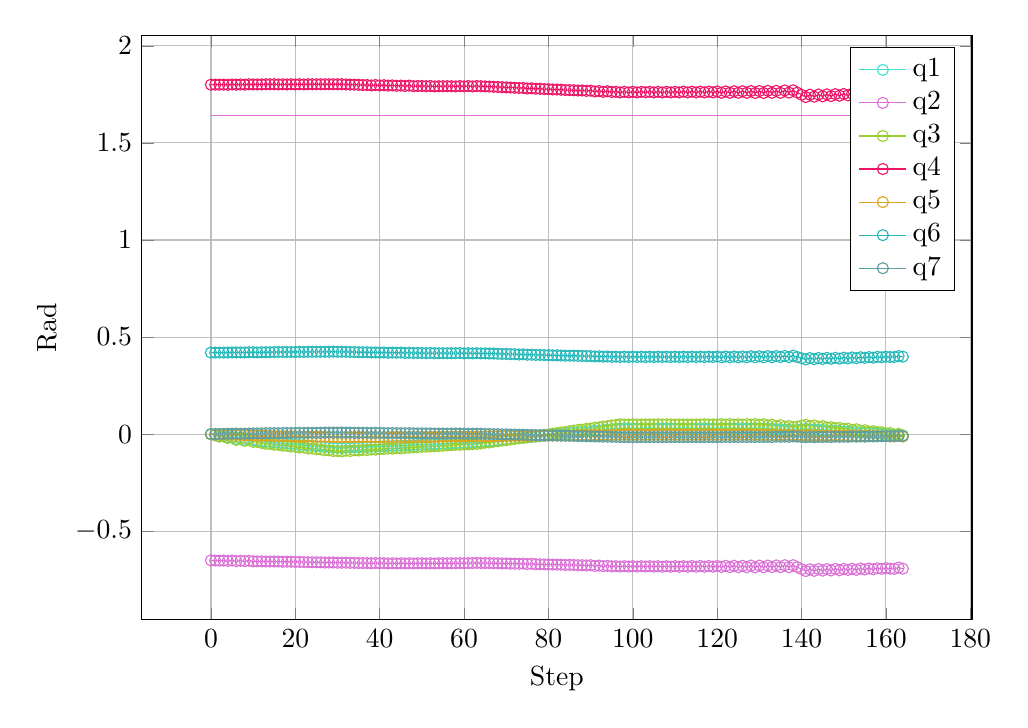
\begin{tikzpicture}
		\begin{axis}[height=9cm, width=\textwidth, grid=major,
		xlabel={Step},ylabel={Rad}
		]
			\addplot [color=Turquoise, mark=o] coordinates {
				(0, 0.000)
				(1, -0.005)
				(2, -0.010)
				(3, -0.010)
				(4, -0.016)
				(5, -0.013)
				(6, -0.024)
				(7, -0.018)
				(8, -0.028)
				(9, -0.022)
				(10, -0.032)
				(11, -0.032)
				(12, -0.036)
				(13, -0.040)
				(14, -0.040)
				(15, -0.044)
				(16, -0.044)
				(17, -0.048)
				(18, -0.048)
				(19, -0.052)
				(20, -0.052)
				(21, -0.056)
				(22, -0.056)
				(23, -0.059)
				(24, -0.060)
				(25, -0.063)
				(26, -0.063)
				(27, -0.066)
				(28, -0.067)
				(29, -0.070)
				(30, -0.070)
				(31, -0.072)
				(32, -0.069)
				(33, -0.070)
				(34, -0.067)
				(35, -0.068)
				(36, -0.066)
				(37, -0.067)
				(38, -0.064)
				(39, -0.065)
				(40, -0.063)
				(41, -0.063)
				(42, -0.061)
				(43, -0.061)
				(44, -0.060)
				(45, -0.060)
				(46, -0.058)
				(47, -0.058)
				(48, -0.056)
				(49, -0.056)
				(50, -0.054)
				(51, -0.054)
				(52, -0.052)
				(53, -0.052)
				(54, -0.051)
				(55, -0.050)
				(56, -0.049)
				(57, -0.048)
				(58, -0.047)
				(59, -0.046)
				(60, -0.045)
				(61, -0.044)
				(62, -0.043)
				(63, -0.042)
				(64, -0.041)
				(65, -0.038)
				(66, -0.037)
				(67, -0.034)
				(68, -0.032)
				(69, -0.030)
				(70, -0.028)
				(71, -0.026)
				(72, -0.023)
				(73, -0.021)
				(74, -0.019)
				(75, -0.017)
				(76, -0.015)
				(77, -0.013)
				(78, -0.011)
				(79, -0.008)
				(80, -0.007)
				(81, -0.004)
				(82, -0.002)
				(83, 0.000)
				(84, 0.002)
				(85, 0.005)
				(86, 0.007)
				(87, 0.009)
				(88, 0.011)
				(89, 0.014)
				(90, 0.015)
				(91, 0.018)
				(92, 0.019)
				(93, 0.022)
				(94, 0.023)
				(95, 0.026)
				(96, 0.027)
				(97, 0.030)
				(98, 0.029)
				(99, 0.030)
				(100, 0.029)
				(101, 0.029)
				(102, 0.029)
				(103, 0.029)
				(104, 0.029)
				(105, 0.029)
				(106, 0.030)
				(107, 0.029)
				(108, 0.030)
				(109, 0.029)
				(110, 0.029)
				(111, 0.029)
				(112, 0.029)
				(113, 0.029)
				(114, 0.029)
				(115, 0.029)
				(116, 0.029)
				(117, 0.030)
				(118, 0.029)
				(119, 0.030)
				(120, 0.029)
				(121, 0.030)
				(122, 0.028)
				(123, 0.030)
				(124, 0.028)
				(125, 0.030)
				(126, 0.029)
				(127, 0.030)
				(128, 0.028)
				(129, 0.031)
				(130, 0.028)
				(131, 0.030)
				(132, 0.026)
				(133, 0.028)
				(134, 0.023)
				(135, 0.026)
				(136, 0.021)
				(137, 0.024)
				(138, 0.019)
				(139, 0.022)
				(140, 0.025)
				(141, 0.028)
				(142, 0.023)
				(143, 0.025)
				(144, 0.021)
				(145, 0.023)
				(146, 0.018)
				(147, 0.020)
				(148, 0.016)
				(149, 0.017)
				(150, 0.013)
				(151, 0.014)
				(152, 0.010)
				(153, 0.012)
				(154, 0.007)
				(155, 0.009)
				(156, 0.004)
				(157, 0.005)
				(158, 0.002)
				(159, 0.001)
				(160, -0.002)
				(161, -0.002)
				(162, -0.008)
				(163, -0.004)
				(164, -0.011)
			};
			\addlegendentry{q1}

			\addplot [color=Orchid, mark=o] coordinates {
				(0, -0.650)
				(1, -0.651)
				(2, -0.652)
				(3, -0.651)
				(4, -0.653)
				(5, -0.651)
				(6, -0.654)
				(7, -0.652)
				(8, -0.654)
				(9, -0.652)
				(10, -0.655)
				(11, -0.655)
				(12, -0.655)
				(13, -0.656)
				(14, -0.656)
				(15, -0.656)
				(16, -0.656)
				(17, -0.657)
				(18, -0.657)
				(19, -0.657)
				(20, -0.658)
				(21, -0.658)
				(22, -0.659)
				(23, -0.659)
				(24, -0.660)
				(25, -0.660)
				(26, -0.660)
				(27, -0.661)
				(28, -0.661)
				(29, -0.661)
				(30, -0.662)
				(31, -0.662)
				(32, -0.662)
				(33, -0.663)
				(34, -0.663)
				(35, -0.664)
				(36, -0.664)
				(37, -0.664)
				(38, -0.665)
				(39, -0.664)
				(40, -0.665)
				(41, -0.664)
				(42, -0.666)
				(43, -0.665)
				(44, -0.666)
				(45, -0.665)
				(46, -0.666)
				(47, -0.665)
				(48, -0.666)
				(49, -0.665)
				(50, -0.665)
				(51, -0.666)
				(52, -0.665)
				(53, -0.666)
				(54, -0.665)
				(55, -0.665)
				(56, -0.665)
				(57, -0.665)
				(58, -0.665)
				(59, -0.664)
				(60, -0.665)
				(61, -0.664)
				(62, -0.664)
				(63, -0.663)
				(64, -0.664)
				(65, -0.664)
				(66, -0.664)
				(67, -0.665)
				(68, -0.665)
				(69, -0.666)
				(70, -0.666)
				(71, -0.667)
				(72, -0.667)
				(73, -0.668)
				(74, -0.667)
				(75, -0.669)
				(76, -0.668)
				(77, -0.670)
				(78, -0.670)
				(79, -0.671)
				(80, -0.671)
				(81, -0.672)
				(82, -0.672)
				(83, -0.672)
				(84, -0.674)
				(85, -0.673)
				(86, -0.674)
				(87, -0.675)
				(88, -0.675)
				(89, -0.676)
				(90, -0.675)
				(91, -0.679)
				(92, -0.677)
				(93, -0.680)
				(94, -0.678)
				(95, -0.681)
				(96, -0.680)
				(97, -0.682)
				(98, -0.680)
				(99, -0.682)
				(100, -0.680)
				(101, -0.682)
				(102, -0.680)
				(103, -0.682)
				(104, -0.680)
				(105, -0.682)
				(106, -0.680)
				(107, -0.683)
				(108, -0.680)
				(109, -0.683)
				(110, -0.680)
				(111, -0.683)
				(112, -0.680)
				(113, -0.683)
				(114, -0.679)
				(115, -0.683)
				(116, -0.679)
				(117, -0.683)
				(118, -0.679)
				(119, -0.683)
				(120, -0.679)
				(121, -0.684)
				(122, -0.678)
				(123, -0.685)
				(124, -0.678)
				(125, -0.685)
				(126, -0.678)
				(127, -0.685)
				(128, -0.677)
				(129, -0.686)
				(130, -0.677)
				(131, -0.686)
				(132, -0.677)
				(133, -0.685)
				(134, -0.676)
				(135, -0.685)
				(136, -0.675)
				(137, -0.685)
				(138, -0.675)
				(139, -0.685)
				(140, -0.695)
				(141, -0.705)
				(142, -0.696)
				(143, -0.704)
				(144, -0.695)
				(145, -0.703)
				(146, -0.695)
				(147, -0.702)
				(148, -0.694)
				(149, -0.701)
				(150, -0.694)
				(151, -0.699)
				(152, -0.693)
				(153, -0.699)
				(154, -0.692)
				(155, -0.697)
				(156, -0.692)
				(157, -0.696)
				(158, -0.691)
				(159, -0.694)
				(160, -0.690)
				(161, -0.693)
				(162, -0.694)
				(163, -0.687)
				(164, -0.693)
			};
			\addlegendentry{q2}

			\addplot [color=YellowGreen, mark=o] coordinates {
				(0, 0.000)
				(1, -0.006)
				(2, -0.013)
				(3, -0.012)
				(4, -0.020)
				(5, -0.017)
				(6, -0.030)
				(7, -0.023)
				(8, -0.035)
				(9, -0.027)
				(10, -0.040)
				(11, -0.040)
				(12, -0.045)
				(13, -0.050)
				(14, -0.050)
				(15, -0.055)
				(16, -0.055)
				(17, -0.060)
				(18, -0.060)
				(19, -0.064)
				(20, -0.065)
				(21, -0.069)
				(22, -0.069)
				(23, -0.074)
				(24, -0.074)
				(25, -0.078)
				(26, -0.079)
				(27, -0.083)
				(28, -0.083)
				(29, -0.087)
				(30, -0.087)
				(31, -0.089)
				(32, -0.085)
				(33, -0.087)
				(34, -0.083)
				(35, -0.084)
				(36, -0.081)
				(37, -0.082)
				(38, -0.079)
				(39, -0.080)
				(40, -0.077)
				(41, -0.077)
				(42, -0.074)
				(43, -0.075)
				(44, -0.072)
				(45, -0.073)
				(46, -0.070)
				(47, -0.070)
				(48, -0.068)
				(49, -0.067)
				(50, -0.065)
				(51, -0.065)
				(52, -0.063)
				(53, -0.062)
				(54, -0.061)
				(55, -0.060)
				(56, -0.058)
				(57, -0.057)
				(58, -0.055)
				(59, -0.055)
				(60, -0.053)
				(61, -0.053)
				(62, -0.051)
				(63, -0.050)
				(64, -0.048)
				(65, -0.044)
				(66, -0.043)
				(67, -0.039)
				(68, -0.037)
				(69, -0.033)
				(70, -0.031)
				(71, -0.027)
				(72, -0.024)
				(73, -0.021)
				(74, -0.019)
				(75, -0.015)
				(76, -0.013)
				(77, -0.009)
				(78, -0.007)
				(79, -0.003)
				(80, -0.002)
				(81, 0.003)
				(82, 0.005)
				(83, 0.009)
				(84, 0.011)
				(85, 0.015)
				(86, 0.018)
				(87, 0.022)
				(88, 0.023)
				(89, 0.027)
				(90, 0.029)
				(91, 0.033)
				(92, 0.035)
				(93, 0.039)
				(94, 0.041)
				(95, 0.045)
				(96, 0.047)
				(97, 0.051)
				(98, 0.050)
				(99, 0.050)
				(100, 0.050)
				(101, 0.050)
				(102, 0.050)
				(103, 0.050)
				(104, 0.050)
				(105, 0.050)
				(106, 0.051)
				(107, 0.050)
				(108, 0.051)
				(109, 0.050)
				(110, 0.050)
				(111, 0.050)
				(112, 0.050)
				(113, 0.050)
				(114, 0.050)
				(115, 0.050)
				(116, 0.050)
				(117, 0.051)
				(118, 0.050)
				(119, 0.050)
				(120, 0.050)
				(121, 0.052)
				(122, 0.049)
				(123, 0.052)
				(124, 0.049)
				(125, 0.051)
				(126, 0.049)
				(127, 0.052)
				(128, 0.049)
				(129, 0.052)
				(130, 0.048)
				(131, 0.051)
				(132, 0.045)
				(133, 0.049)
				(134, 0.041)
				(135, 0.046)
				(136, 0.038)
				(137, 0.042)
				(138, 0.035)
				(139, 0.039)
				(140, 0.044)
				(141, 0.048)
				(142, 0.041)
				(143, 0.045)
				(144, 0.038)
				(145, 0.041)
				(146, 0.034)
				(147, 0.036)
				(148, 0.031)
				(149, 0.032)
				(150, 0.027)
				(151, 0.028)
				(152, 0.022)
				(153, 0.025)
				(154, 0.018)
				(155, 0.020)
				(156, 0.013)
				(157, 0.015)
				(158, 0.010)
				(159, 0.010)
				(160, 0.004)
				(161, 0.006)
				(162, -0.003)
				(163, 0.002)
				(164, -0.007)
			};
			\addlegendentry{q3}

			\addplot [color=WildStrawberry, mark=o] coordinates {
				(0, 1.800)
				(1, 1.800)
				(2, 1.800)
				(3, 1.800)
				(4, 1.799)
				(5, 1.801)
				(6, 1.800)
				(7, 1.801)
				(8, 1.800)
				(9, 1.802)
				(10, 1.801)
				(11, 1.801)
				(12, 1.801)
				(13, 1.802)
				(14, 1.802)
				(15, 1.802)
				(16, 1.801)
				(17, 1.802)
				(18, 1.801)
				(19, 1.802)
				(20, 1.801)
				(21, 1.802)
				(22, 1.801)
				(23, 1.802)
				(24, 1.802)
				(25, 1.802)
				(26, 1.802)
				(27, 1.802)
				(28, 1.802)
				(29, 1.802)
				(30, 1.802)
				(31, 1.802)
				(32, 1.801)
				(33, 1.800)
				(34, 1.800)
				(35, 1.799)
				(36, 1.798)
				(37, 1.798)
				(38, 1.796)
				(39, 1.798)
				(40, 1.796)
				(41, 1.797)
				(42, 1.795)
				(43, 1.796)
				(44, 1.794)
				(45, 1.795)
				(46, 1.793)
				(47, 1.795)
				(48, 1.792)
				(49, 1.793)
				(50, 1.793)
				(51, 1.792)
				(52, 1.793)
				(53, 1.791)
				(54, 1.792)
				(55, 1.792)
				(56, 1.792)
				(57, 1.792)
				(58, 1.791)
				(59, 1.793)
				(60, 1.791)
				(61, 1.793)
				(62, 1.791)
				(63, 1.793)
				(64, 1.792)
				(65, 1.791)
				(66, 1.790)
				(67, 1.789)
				(68, 1.788)
				(69, 1.787)
				(70, 1.786)
				(71, 1.785)
				(72, 1.784)
				(73, 1.783)
				(74, 1.783)
				(75, 1.780)
				(76, 1.781)
				(77, 1.779)
				(78, 1.779)
				(79, 1.777)
				(80, 1.777)
				(81, 1.775)
				(82, 1.775)
				(83, 1.774)
				(84, 1.772)
				(85, 1.772)
				(86, 1.771)
				(87, 1.770)
				(88, 1.770)
				(89, 1.768)
				(90, 1.769)
				(91, 1.765)
				(92, 1.767)
				(93, 1.763)
				(94, 1.766)
				(95, 1.762)
				(96, 1.763)
				(97, 1.760)
				(98, 1.763)
				(99, 1.760)
				(100, 1.763)
				(101, 1.760)
				(102, 1.763)
				(103, 1.761)
				(104, 1.763)
				(105, 1.760)
				(106, 1.763)
				(107, 1.760)
				(108, 1.763)
				(109, 1.760)
				(110, 1.763)
				(111, 1.760)
				(112, 1.764)
				(113, 1.760)
				(114, 1.764)
				(115, 1.760)
				(116, 1.764)
				(117, 1.760)
				(118, 1.764)
				(119, 1.760)
				(120, 1.765)
				(121, 1.758)
				(122, 1.765)
				(123, 1.758)
				(124, 1.766)
				(125, 1.758)
				(126, 1.766)
				(127, 1.758)
				(128, 1.767)
				(129, 1.757)
				(130, 1.767)
				(131, 1.757)
				(132, 1.768)
				(133, 1.758)
				(134, 1.768)
				(135, 1.758)
				(136, 1.770)
				(137, 1.759)
				(138, 1.771)
				(139, 1.759)
				(140, 1.748)
				(141, 1.736)
				(142, 1.748)
				(143, 1.738)
				(144, 1.749)
				(145, 1.740)
				(146, 1.750)
				(147, 1.741)
				(148, 1.751)
				(149, 1.743)
				(150, 1.752)
				(151, 1.745)
				(152, 1.754)
				(153, 1.747)
				(154, 1.755)
				(155, 1.749)
				(156, 1.756)
				(157, 1.751)
				(158, 1.757)
				(159, 1.754)
				(160, 1.759)
				(161, 1.756)
				(162, 1.755)
				(163, 1.763)
				(164, 1.758)
			};
			\addlegendentry{q4}

			\addplot [color=Goldenrod, mark=o] coordinates {
				(0, 0.000)
				(1, -0.001)
				(2, -0.002)
				(3, -0.002)
				(4, -0.004)
				(5, -0.003)
				(6, -0.005)
				(7, -0.004)
				(8, -0.006)
				(9, -0.005)
				(10, -0.007)
				(11, -0.007)
				(12, -0.008)
				(13, -0.009)
				(14, -0.009)
				(15, -0.010)
				(16, -0.010)
				(17, -0.010)
				(18, -0.010)
				(19, -0.011)
				(20, -0.011)
				(21, -0.012)
				(22, -0.012)
				(23, -0.013)
				(24, -0.013)
				(25, -0.014)
				(26, -0.014)
				(27, -0.014)
				(28, -0.015)
				(29, -0.015)
				(30, -0.015)
				(31, -0.016)
				(32, -0.015)
				(33, -0.016)
				(34, -0.015)
				(35, -0.016)
				(36, -0.015)
				(37, -0.015)
				(38, -0.015)
				(39, -0.015)
				(40, -0.015)
				(41, -0.015)
				(42, -0.015)
				(43, -0.015)
				(44, -0.015)
				(45, -0.014)
				(46, -0.015)
				(47, -0.014)
				(48, -0.014)
				(49, -0.014)
				(50, -0.014)
				(51, -0.014)
				(52, -0.014)
				(53, -0.014)
				(54, -0.013)
				(55, -0.013)
				(56, -0.013)
				(57, -0.013)
				(58, -0.013)
				(59, -0.012)
				(60, -0.012)
				(61, -0.012)
				(62, -0.012)
				(63, -0.012)
				(64, -0.012)
				(65, -0.011)
				(66, -0.011)
				(67, -0.011)
				(68, -0.010)
				(69, -0.010)
				(70, -0.010)
				(71, -0.010)
				(72, -0.009)
				(73, -0.009)
				(74, -0.009)
				(75, -0.009)
				(76, -0.009)
				(77, -0.008)
				(78, -0.008)
				(79, -0.008)
				(80, -0.008)
				(81, -0.007)
				(82, -0.007)
				(83, -0.007)
				(84, -0.007)
				(85, -0.007)
				(86, -0.006)
				(87, -0.006)
				(88, -0.006)
				(89, -0.006)
				(90, -0.006)
				(91, -0.005)
				(92, -0.005)
				(93, -0.005)
				(94, -0.005)
				(95, -0.005)
				(96, -0.004)
				(97, -0.004)
				(98, -0.004)
				(99, -0.004)
				(100, -0.004)
				(101, -0.004)
				(102, -0.004)
				(103, -0.004)
				(104, -0.004)
				(105, -0.004)
				(106, -0.004)
				(107, -0.004)
				(108, -0.004)
				(109, -0.004)
				(110, -0.004)
				(111, -0.004)
				(112, -0.004)
				(113, -0.004)
				(114, -0.004)
				(115, -0.004)
				(116, -0.004)
				(117, -0.004)
				(118, -0.004)
				(119, -0.004)
				(120, -0.004)
				(121, -0.004)
				(122, -0.004)
				(123, -0.004)
				(124, -0.004)
				(125, -0.004)
				(126, -0.004)
				(127, -0.004)
				(128, -0.004)
				(129, -0.004)
				(130, -0.004)
				(131, -0.005)
				(132, -0.004)
				(133, -0.005)
				(134, -0.005)
				(135, -0.005)
				(136, -0.005)
				(137, -0.005)
				(138, -0.005)
				(139, -0.006)
				(140, -0.006)
				(141, -0.006)
				(142, -0.006)
				(143, -0.007)
				(144, -0.007)
				(145, -0.007)
				(146, -0.007)
				(147, -0.007)
				(148, -0.007)
				(149, -0.008)
				(150, -0.008)
				(151, -0.008)
				(152, -0.008)
				(153, -0.009)
				(154, -0.009)
				(155, -0.009)
				(156, -0.009)
				(157, -0.010)
				(158, -0.010)
				(159, -0.010)
				(160, -0.010)
				(161, -0.011)
				(162, -0.012)
				(163, -0.010)
				(164, -0.012)
			};
			\addlegendentry{q5}

			\addplot [color=BlueGreen, mark=o] coordinates {
				(0, 0.420)
				(1, 0.420)
				(2, 0.420)
				(3, 0.420)
				(4, 0.420)
				(5, 0.421)
				(6, 0.421)
				(7, 0.421)
				(8, 0.421)
				(9, 0.422)
				(10, 0.422)
				(11, 0.421)
				(12, 0.422)
				(13, 0.422)
				(14, 0.422)
				(15, 0.423)
				(16, 0.423)
				(17, 0.423)
				(18, 0.423)
				(19, 0.423)
				(20, 0.423)
				(21, 0.424)
				(22, 0.423)
				(23, 0.424)
				(24, 0.424)
				(25, 0.424)
				(26, 0.424)
				(27, 0.424)
				(28, 0.424)
				(29, 0.425)
				(30, 0.424)
				(31, 0.424)
				(32, 0.424)
				(33, 0.423)
				(34, 0.423)
				(35, 0.422)
				(36, 0.422)
				(37, 0.422)
				(38, 0.421)
				(39, 0.421)
				(40, 0.420)
				(41, 0.421)
				(42, 0.419)
				(43, 0.420)
				(44, 0.419)
				(45, 0.420)
				(46, 0.418)
				(47, 0.419)
				(48, 0.418)
				(49, 0.418)
				(50, 0.418)
				(51, 0.417)
				(52, 0.418)
				(53, 0.417)
				(54, 0.417)
				(55, 0.417)
				(56, 0.417)
				(57, 0.417)
				(58, 0.417)
				(59, 0.418)
				(60, 0.416)
				(61, 0.417)
				(62, 0.416)
				(63, 0.417)
				(64, 0.416)
				(65, 0.416)
				(66, 0.415)
				(67, 0.415)
				(68, 0.414)
				(69, 0.413)
				(70, 0.413)
				(71, 0.412)
				(72, 0.412)
				(73, 0.410)
				(74, 0.411)
				(75, 0.409)
				(76, 0.409)
				(77, 0.408)
				(78, 0.408)
				(79, 0.407)
				(80, 0.407)
				(81, 0.406)
				(82, 0.406)
				(83, 0.405)
				(84, 0.404)
				(85, 0.404)
				(86, 0.404)
				(87, 0.403)
				(88, 0.403)
				(89, 0.402)
				(90, 0.402)
				(91, 0.400)
				(92, 0.401)
				(93, 0.399)
				(94, 0.400)
				(95, 0.398)
				(96, 0.399)
				(97, 0.397)
				(98, 0.399)
				(99, 0.397)
				(100, 0.399)
				(101, 0.397)
				(102, 0.399)
				(103, 0.397)
				(104, 0.399)
				(105, 0.397)
				(106, 0.399)
				(107, 0.397)
				(108, 0.399)
				(109, 0.397)
				(110, 0.399)
				(111, 0.397)
				(112, 0.399)
				(113, 0.397)
				(114, 0.399)
				(115, 0.397)
				(116, 0.399)
				(117, 0.397)
				(118, 0.399)
				(119, 0.397)
				(120, 0.400)
				(121, 0.396)
				(122, 0.400)
				(123, 0.396)
				(124, 0.400)
				(125, 0.396)
				(126, 0.400)
				(127, 0.396)
				(128, 0.401)
				(129, 0.396)
				(130, 0.401)
				(131, 0.396)
				(132, 0.402)
				(133, 0.396)
				(134, 0.402)
				(135, 0.397)
				(136, 0.403)
				(137, 0.397)
				(138, 0.404)
				(139, 0.397)
				(140, 0.391)
				(141, 0.385)
				(142, 0.392)
				(143, 0.386)
				(144, 0.392)
				(145, 0.387)
				(146, 0.393)
				(147, 0.388)
				(148, 0.393)
				(149, 0.389)
				(150, 0.394)
				(151, 0.390)
				(152, 0.395)
				(153, 0.391)
				(154, 0.396)
				(155, 0.393)
				(156, 0.397)
				(157, 0.394)
				(158, 0.398)
				(159, 0.396)
				(160, 0.399)
				(161, 0.397)
				(162, 0.397)
				(163, 0.402)
				(164, 0.399)
			};
			\addlegendentry{q6}

			\addplot [color=CadetBlue, mark=o] coordinates {
				(0, 0.000)
				(1, 0.001)
				(2, 0.001)
				(3, 0.001)
				(4, 0.002)
				(5, 0.002)
				(6, 0.003)
				(7, 0.002)
				(8, 0.003)
				(9, 0.003)
				(10, 0.004)
				(11, 0.004)
				(12, 0.004)
				(13, 0.005)
				(14, 0.005)
				(15, 0.005)
				(16, 0.005)
				(17, 0.006)
				(18, 0.006)
				(19, 0.006)
				(20, 0.006)
				(21, 0.007)
				(22, 0.006)
				(23, 0.007)
				(24, 0.007)
				(25, 0.007)
				(26, 0.007)
				(27, 0.008)
				(28, 0.008)
				(29, 0.008)
				(30, 0.008)
				(31, 0.008)
				(32, 0.008)
				(33, 0.008)
				(34, 0.007)
				(35, 0.007)
				(36, 0.007)
				(37, 0.007)
				(38, 0.006)
				(39, 0.007)
				(40, 0.006)
				(41, 0.006)
				(42, 0.005)
				(43, 0.006)
				(44, 0.005)
				(45, 0.005)
				(46, 0.005)
				(47, 0.005)
				(48, 0.004)
				(49, 0.004)
				(50, 0.004)
				(51, 0.004)
				(52, 0.004)
				(53, 0.003)
				(54, 0.003)
				(55, 0.003)
				(56, 0.003)
				(57, 0.003)
				(58, 0.003)
				(59, 0.003)
				(60, 0.002)
				(61, 0.002)
				(62, 0.002)
				(63, 0.002)
				(64, 0.002)
				(65, 0.001)
				(66, 0.001)
				(67, 0.000)
				(68, -0.000)
				(69, -0.001)
				(70, -0.001)
				(71, -0.002)
				(72, -0.002)
				(73, -0.003)
				(74, -0.003)
				(75, -0.004)
				(76, -0.004)
				(77, -0.005)
				(78, -0.005)
				(79, -0.006)
				(80, -0.006)
				(81, -0.007)
				(82, -0.007)
				(83, -0.008)
				(84, -0.008)
				(85, -0.009)
				(86, -0.009)
				(87, -0.010)
				(88, -0.010)
				(89, -0.011)
				(90, -0.011)
				(91, -0.012)
				(92, -0.012)
				(93, -0.013)
				(94, -0.013)
				(95, -0.014)
				(96, -0.014)
				(97, -0.015)
				(98, -0.015)
				(99, -0.015)
				(100, -0.015)
				(101, -0.015)
				(102, -0.015)
				(103, -0.015)
				(104, -0.015)
				(105, -0.015)
				(106, -0.015)
				(107, -0.015)
				(108, -0.015)
				(109, -0.015)
				(110, -0.015)
				(111, -0.015)
				(112, -0.015)
				(113, -0.015)
				(114, -0.015)
				(115, -0.015)
				(116, -0.015)
				(117, -0.015)
				(118, -0.015)
				(119, -0.015)
				(120, -0.015)
				(121, -0.015)
				(122, -0.014)
				(123, -0.015)
				(124, -0.014)
				(125, -0.015)
				(126, -0.014)
				(127, -0.015)
				(128, -0.014)
				(129, -0.015)
				(130, -0.014)
				(131, -0.015)
				(132, -0.014)
				(133, -0.015)
				(134, -0.013)
				(135, -0.014)
				(136, -0.013)
				(137, -0.014)
				(138, -0.012)
				(139, -0.013)
				(140, -0.015)
				(141, -0.016)
				(142, -0.014)
				(143, -0.016)
				(144, -0.014)
				(145, -0.015)
				(146, -0.014)
				(147, -0.015)
				(148, -0.013)
				(149, -0.014)
				(150, -0.013)
				(151, -0.014)
				(152, -0.012)
				(153, -0.013)
				(154, -0.012)
				(155, -0.013)
				(156, -0.011)
				(157, -0.012)
				(158, -0.011)
				(159, -0.011)
				(160, -0.010)
				(161, -0.011)
				(162, -0.010)
				(163, -0.009)
				(164, -0.009)
			};
			\addlegendentry{q7}

			\addplot[Turquoise,sharp plot,update limits=false] coordinates {				(0,3.14)
				(160,3.14)
			};
			\addplot[Turquoise,sharp plot,update limits=false] coordinates {				(0,-3.14)
				(160,-3.14)
			};

			\addplot[Orchid,sharp plot,update limits=false] coordinates {				(0,1.64)
				(160,1.64)
			};
			\addplot[Orchid,sharp plot,update limits=false] coordinates {				(0,-1.64)
				(160,-1.64)
			};

			\addplot[YellowGreen,sharp plot,update limits=false] coordinates {				(0,3.14)
				(160,3.14)
			};
			\addplot[YellowGreen,sharp plot,update limits=false] coordinates {				(0,-3.14)
				(160,-3.14)
			};

			\addplot[WildStrawberry,sharp plot,update limits=false] coordinates {				(0,2.5)
				(160,2.5)
			};
			\addplot[WildStrawberry,sharp plot,update limits=false] coordinates {				(0,-2.5)
				(160,-2.5)
			};

			\addplot[Goldenrod,sharp plot,update limits=false] coordinates {				(0,4.71)
				(160,4.71)
			};
			\addplot[Goldenrod,sharp plot,update limits=false] coordinates {				(0,-4.71)
				(160,-4.71)
			};

			\addplot[BlueGreen,sharp plot,update limits=false] coordinates {				(0,2.09)
				(160,2.09)
			};
			\addplot[BlueGreen,sharp plot,update limits=false] coordinates {				(0,-2.09)
				(160,-2.09)
			};

			\addplot[CadetBlue,sharp plot,update limits=false] coordinates {				(0,6.28)
				(160,6.28)
			};
			\addplot[CadetBlue,sharp plot,update limits=false] coordinates {
				(0,-6.28)
				(160,-6.28)
			};
		\end{axis}
	\end{tikzpicture}
	\caption{Robot's state while tracking the corny marker at medium speed.}
	\label{fig:qRobotCornyMediumPlot}
\end{figure}
}

\providecommand{\speedCornyMediumPlot}{
\begin{figure}[!ht]
	\centering
	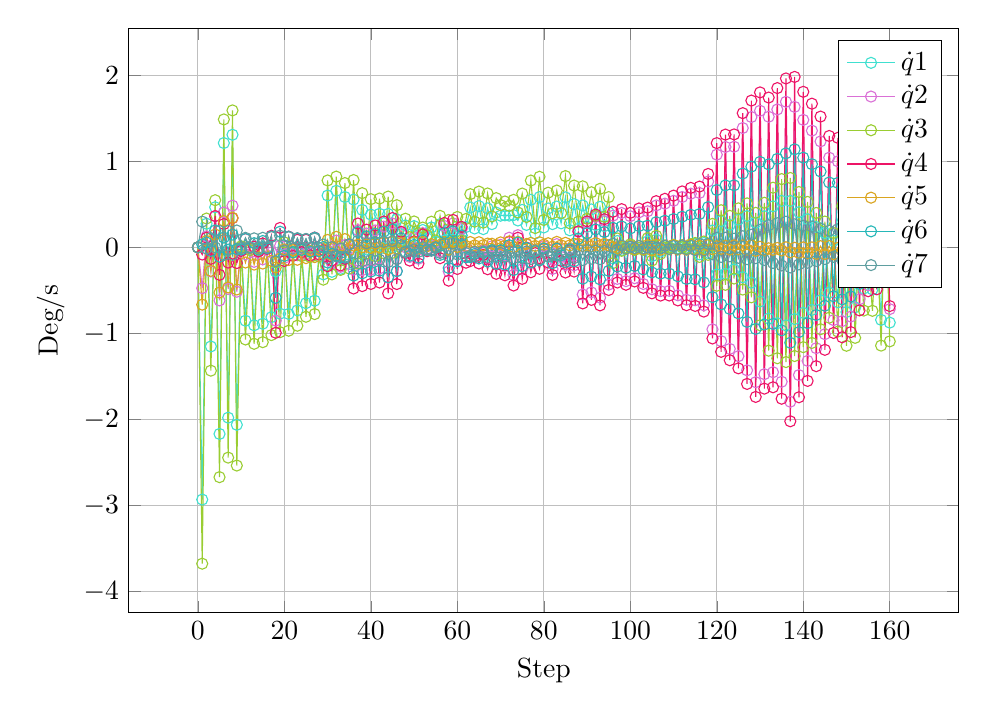
\begin{tikzpicture}
		\begin{axis}[height=9cm, width=\textwidth, grid=major,
		xlabel={Step},ylabel={Deg/s}
		]
			\addplot [color=Turquoise, mark=o] coordinates {
				(0, 0.000)
				(1, -2.929)
				(2, 0.275)
				(3, -1.151)
				(4, 0.466)
				(5, -2.167)
				(6, 1.212)
				(7, -1.978)
				(8, 1.308)
				(9, -2.061)
				(10, 0.006)
				(11, -0.852)
				(12, -0.026)
				(13, -0.905)
				(14, -0.042)
				(15, -0.887)
				(16, -0.011)
				(17, -0.811)
				(18, -0.279)
				(19, -0.770)
				(20, 0.024)
				(21, -0.773)
				(22, -0.061)
				(23, -0.732)
				(24, -0.093)
				(25, -0.648)
				(26, -0.107)
				(27, -0.619)
				(28, -0.101)
				(29, -0.314)
				(30, 0.602)
				(31, -0.284)
				(32, 0.657)
				(33, -0.249)
				(34, 0.585)
				(35, -0.194)
				(36, 0.555)
				(37, -0.105)
				(38, 0.435)
				(39, -0.024)
				(40, 0.381)
				(41, -0.042)
				(42, 0.390)
				(43, -0.008)
				(44, 0.388)
				(45, 0.001)
				(46, 0.325)
				(47, 0.082)
				(48, 0.254)
				(49, 0.071)
				(50, 0.247)
				(51, 0.104)
				(52, 0.202)
				(53, 0.106)
				(54, 0.231)
				(55, 0.064)
				(56, 0.270)
				(57, 0.079)
				(58, 0.198)
				(59, 0.088)
				(60, 0.244)
				(61, 0.092)
				(62, 0.236)
				(63, 0.463)
				(64, 0.219)
				(65, 0.479)
				(66, 0.212)
				(67, 0.453)
				(68, 0.270)
				(69, 0.404)
				(70, 0.368)
				(71, 0.372)
				(72, 0.369)
				(73, 0.375)
				(74, 0.312)
				(75, 0.435)
				(76, 0.261)
				(77, 0.552)
				(78, 0.160)
				(79, 0.584)
				(80, 0.231)
				(81, 0.452)
				(82, 0.270)
				(83, 0.474)
				(84, 0.279)
				(85, 0.581)
				(86, 0.198)
				(87, 0.502)
				(88, 0.216)
				(89, 0.487)
				(90, 0.239)
				(91, 0.441)
				(92, 0.260)
				(93, 0.471)
				(94, 0.246)
				(95, 0.407)
				(96, -0.129)
				(97, 0.074)
				(98, -0.030)
				(99, -0.002)
				(100, 0.023)
				(101, -0.018)
				(102, -0.007)
				(103, -0.017)
				(104, 0.071)
				(105, -0.103)
				(106, 0.090)
				(107, -0.049)
				(108, -0.004)
				(109, 0.001)
				(110, 0.017)
				(111, -0.009)
				(112, -0.002)
				(113, -0.002)
				(114, 0.022)
				(115, 0.040)
				(116, -0.081)
				(117, 0.051)
				(118, -0.065)
				(119, 0.196)
				(120, -0.314)
				(121, 0.305)
				(122, -0.308)
				(123, 0.261)
				(124, -0.257)
				(125, 0.322)
				(126, -0.347)
				(127, 0.364)
				(128, -0.410)
				(129, 0.287)
				(130, -0.629)
				(131, 0.362)
				(132, -0.826)
				(133, 0.477)
				(134, -0.881)
				(135, 0.540)
				(136, -0.906)
				(137, 0.539)
				(138, -0.833)
				(139, 0.409)
				(140, -0.760)
				(141, 0.327)
				(142, -0.726)
				(143, 0.236)
				(144, -0.615)
				(145, 0.167)
				(146, -0.526)
				(147, 0.077)
				(148, -0.638)
				(149, 0.293)
				(150, -0.751)
				(151, 0.251)
				(152, -0.697)
				(153, 0.112)
				(154, -0.478)
				(155, -0.090)
				(156, -0.489)
				(157, 0.097)
				(158, -0.842)
				(159, 0.511)
				(160, -0.874)
			};
			\addlegendentry{$\dot q$1}

			\addplot [color=Orchid, mark=o] coordinates {
				(0, 0.000)
				(1, -0.474)
				(2, 0.128)
				(3, -0.280)
				(4, 0.362)
				(5, -0.616)
				(6, 0.405)
				(7, -0.484)
				(8, 0.484)
				(9, -0.515)
				(10, -0.032)
				(11, -0.080)
				(12, -0.010)
				(13, -0.168)
				(14, -0.046)
				(15, -0.140)
				(16, -0.016)
				(17, -0.058)
				(18, -0.851)
				(19, 0.018)
				(20, -0.122)
				(21, -0.067)
				(22, -0.092)
				(23, -0.091)
				(24, -0.065)
				(25, -0.076)
				(26, -0.098)
				(27, -0.052)
				(28, -0.088)
				(29, -0.095)
				(30, -0.036)
				(31, -0.187)
				(32, 0.079)
				(33, -0.226)
				(34, 0.027)
				(35, -0.016)
				(36, -0.259)
				(37, 0.199)
				(38, -0.265)
				(39, 0.161)
				(40, -0.259)
				(41, 0.197)
				(42, -0.245)
				(43, 0.241)
				(44, -0.350)
				(45, 0.278)
				(46, -0.276)
				(47, 0.166)
				(48, 0.000)
				(49, -0.111)
				(50, 0.109)
				(51, -0.132)
				(52, 0.166)
				(53, -0.015)
				(54, 0.025)
				(55, 0.018)
				(56, -0.048)
				(57, 0.249)
				(58, -0.279)
				(59, 0.279)
				(60, -0.159)
				(61, 0.214)
				(62, -0.101)
				(63, -0.044)
				(64, -0.053)
				(65, -0.068)
				(66, -0.034)
				(67, -0.133)
				(68, 0.013)
				(69, -0.191)
				(70, 0.029)
				(71, -0.215)
				(72, 0.112)
				(73, -0.321)
				(74, 0.142)
				(75, -0.252)
				(76, 0.034)
				(77, -0.176)
				(78, -0.037)
				(79, -0.145)
				(80, 0.015)
				(81, -0.102)
				(82, -0.251)
				(83, 0.038)
				(84, -0.111)
				(85, -0.205)
				(86, -0.013)
				(87, -0.209)
				(88, 0.181)
				(89, -0.547)
				(90, 0.284)
				(91, -0.522)
				(92, 0.356)
				(93, -0.585)
				(94, 0.304)
				(95, -0.433)
				(96, 0.368)
				(97, -0.366)
				(98, 0.399)
				(99, -0.392)
				(100, 0.362)
				(101, -0.358)
				(102, 0.406)
				(103, -0.425)
				(104, 0.419)
				(105, -0.486)
				(106, 0.487)
				(107, -0.508)
				(108, 0.508)
				(109, -0.505)
				(110, 0.541)
				(111, -0.557)
				(112, 0.585)
				(113, -0.608)
				(114, 0.623)
				(115, -0.614)
				(116, 0.632)
				(117, -0.673)
				(118, 0.765)
				(119, -0.952)
				(120, 1.077)
				(121, -1.089)
				(122, 1.166)
				(123, -1.179)
				(124, 1.169)
				(125, -1.264)
				(126, 1.386)
				(127, -1.428)
				(128, 1.514)
				(129, -1.566)
				(130, 1.587)
				(131, -1.473)
				(132, 1.517)
				(133, -1.450)
				(134, 1.602)
				(135, -1.561)
				(136, 1.691)
				(137, -1.793)
				(138, 1.632)
				(139, -1.483)
				(140, 1.481)
				(141, -1.318)
				(142, 1.356)
				(143, -1.171)
				(144, 1.231)
				(145, -1.008)
				(146, 1.042)
				(147, -0.845)
				(148, 0.999)
				(149, -0.857)
				(150, 1.032)
				(151, -0.804)
				(152, 0.826)
				(153, -0.603)
				(154, 0.697)
				(155, -0.441)
				(156, 0.550)
				(157, -0.392)
				(158, -0.199)
				(159, 0.976)
				(160, -0.717)
			};
			\addlegendentry{$\dot q$2}

			\addplot [color=YellowGreen, mark=o] coordinates {
				(0, 0.000)
				(1, -3.674)
				(2, 0.335)
				(3, -1.432)
				(4, 0.548)
				(5, -2.669)
				(6, 1.486)
				(7, -2.442)
				(8, 1.591)
				(9, -2.534)
				(10, 0.013)
				(11, -1.070)
				(12, -0.031)
				(13, -1.120)
				(14, -0.044)
				(15, -1.101)
				(16, -0.011)
				(17, -1.019)
				(18, -0.173)
				(19, -0.985)
				(20, 0.058)
				(21, -0.968)
				(22, -0.056)
				(23, -0.910)
				(24, -0.102)
				(25, -0.806)
				(26, -0.112)
				(27, -0.775)
				(28, -0.106)
				(29, -0.375)
				(30, 0.777)
				(31, -0.314)
				(32, 0.822)
				(33, -0.262)
				(34, 0.747)
				(35, -0.246)
				(36, 0.782)
				(37, -0.185)
				(38, 0.630)
				(39, -0.070)
				(40, 0.560)
				(41, -0.102)
				(42, 0.567)
				(43, -0.068)
				(44, 0.590)
				(45, -0.064)
				(46, 0.490)
				(47, 0.070)
				(48, 0.333)
				(49, 0.118)
				(50, 0.301)
				(51, 0.166)
				(52, 0.230)
				(53, 0.142)
				(54, 0.298)
				(55, 0.080)
				(56, 0.366)
				(57, 0.053)
				(58, 0.318)
				(59, 0.060)
				(60, 0.353)
				(61, 0.079)
				(62, 0.330)
				(63, 0.618)
				(64, 0.299)
				(65, 0.648)
				(66, 0.287)
				(67, 0.626)
				(68, 0.359)
				(69, 0.572)
				(70, 0.491)
				(71, 0.533)
				(72, 0.483)
				(73, 0.552)
				(74, 0.406)
				(75, 0.625)
				(76, 0.353)
				(77, 0.776)
				(78, 0.224)
				(79, 0.820)
				(80, 0.318)
				(81, 0.635)
				(82, 0.396)
				(83, 0.660)
				(84, 0.398)
				(85, 0.828)
				(86, 0.279)
				(87, 0.718)
				(88, 0.298)
				(89, 0.709)
				(90, 0.332)
				(91, 0.640)
				(92, 0.367)
				(93, 0.680)
				(94, 0.355)
				(95, 0.584)
				(96, -0.183)
				(97, 0.103)
				(98, -0.040)
				(99, -0.006)
				(100, 0.036)
				(101, -0.030)
				(102, -0.006)
				(103, -0.028)
				(104, 0.107)
				(105, -0.153)
				(106, 0.135)
				(107, -0.075)
				(108, -0.001)
				(109, -0.003)
				(110, 0.030)
				(111, -0.018)
				(112, 0.003)
				(113, -0.008)
				(114, 0.037)
				(115, 0.051)
				(116, -0.111)
				(117, 0.068)
				(118, -0.087)
				(119, 0.273)
				(120, -0.446)
				(121, 0.431)
				(122, -0.435)
				(123, 0.366)
				(124, -0.362)
				(125, 0.453)
				(126, -0.490)
				(127, 0.511)
				(128, -0.580)
				(129, 0.401)
				(130, -0.905)
				(131, 0.518)
				(132, -1.200)
				(133, 0.693)
				(134, -1.288)
				(135, 0.793)
				(136, -1.332)
				(137, 0.806)
				(138, -1.262)
				(139, 0.643)
				(140, -1.159)
				(141, 0.528)
				(142, -1.110)
				(143, 0.400)
				(144, -0.951)
				(145, 0.300)
				(146, -0.817)
				(147, 0.168)
				(148, -0.978)
				(149, 0.480)
				(150, -1.143)
				(151, 0.421)
				(152, -1.051)
				(153, 0.214)
				(154, -0.734)
				(155, -0.077)
				(156, -0.737)
				(157, 0.179)
				(158, -1.141)
				(159, 0.576)
				(160, -1.092)
			};
			\addlegendentry{$\dot q$3}

			\addplot [color=WildStrawberry, mark=o] coordinates {
				(0, 0.000)
				(1, -0.083)
				(2, 0.112)
				(3, -0.134)
				(4, 0.364)
				(5, -0.319)
				(6, 0.271)
				(7, -0.177)
				(8, 0.340)
				(9, -0.182)
				(10, -0.041)
				(11, 0.096)
				(12, -0.007)
				(13, 0.008)
				(14, -0.047)
				(15, 0.046)
				(16, -0.017)
				(17, 0.135)
				(18, -0.992)
				(19, 0.226)
				(20, -0.159)
				(21, 0.125)
				(22, -0.098)
				(23, 0.088)
				(24, -0.056)
				(25, 0.088)
				(26, -0.093)
				(27, 0.114)
				(28, -0.081)
				(29, -0.028)
				(30, -0.219)
				(31, -0.152)
				(32, -0.089)
				(33, -0.210)
				(34, -0.133)
				(35, 0.035)
				(36, -0.478)
				(37, 0.277)
				(38, -0.450)
				(39, 0.206)
				(40, -0.425)
				(41, 0.255)
				(42, -0.408)
				(43, 0.300)
				(44, -0.535)
				(45, 0.341)
				(46, -0.426)
				(47, 0.181)
				(48, -0.067)
				(49, -0.154)
				(50, 0.069)
				(51, -0.188)
				(52, 0.151)
				(53, -0.045)
				(54, -0.028)
				(55, 0.006)
				(56, -0.126)
				(57, 0.284)
				(58, -0.387)
				(59, 0.319)
				(60, -0.251)
				(61, 0.238)
				(62, -0.178)
				(63, -0.159)
				(64, -0.114)
				(65, -0.187)
				(66, -0.087)
				(67, -0.254)
				(68, -0.041)
				(69, -0.307)
				(70, -0.038)
				(71, -0.324)
				(72, 0.064)
				(73, -0.443)
				(74, 0.112)
				(75, -0.366)
				(76, -0.003)
				(77, -0.289)
				(78, -0.067)
				(79, -0.249)
				(80, -0.015)
				(81, -0.176)
				(82, -0.320)
				(83, -0.012)
				(84, -0.157)
				(85, -0.292)
				(86, -0.034)
				(87, -0.281)
				(88, 0.186)
				(89, -0.651)
				(90, 0.302)
				(91, -0.610)
				(92, 0.382)
				(93, -0.674)
				(94, 0.327)
				(95, -0.495)
				(96, 0.413)
				(97, -0.408)
				(98, 0.444)
				(99, -0.434)
				(100, 0.401)
				(101, -0.396)
				(102, 0.451)
				(103, -0.470)
				(104, 0.462)
				(105, -0.534)
				(106, 0.537)
				(107, -0.560)
				(108, 0.564)
				(109, -0.559)
				(110, 0.601)
				(111, -0.616)
				(112, 0.650)
				(113, -0.672)
				(114, 0.691)
				(115, -0.680)
				(116, 0.706)
				(117, -0.746)
				(118, 0.853)
				(119, -1.058)
				(120, 1.211)
				(121, -1.213)
				(122, 1.310)
				(123, -1.311)
				(124, 1.312)
				(125, -1.405)
				(126, 1.559)
				(127, -1.586)
				(128, 1.705)
				(129, -1.737)
				(130, 1.800)
				(131, -1.641)
				(132, 1.740)
				(133, -1.625)
				(134, 1.850)
				(135, -1.758)
				(136, 1.962)
				(137, -2.020)
				(138, 1.980)
				(139, -1.741)
				(140, 1.807)
				(141, -1.551)
				(142, 1.669)
				(143, -1.380)
				(144, 1.519)
				(145, -1.190)
				(146, 1.294)
				(147, -0.994)
				(148, 1.272)
				(149, -1.044)
				(150, 1.339)
				(151, -0.984)
				(152, 1.098)
				(153, -0.732)
				(154, 0.914)
				(155, -0.509)
				(156, 0.751)
				(157, -0.487)
				(158, -0.068)
				(159, 1.085)
				(160, -0.682)
			};
			\addlegendentry{$\dot q$4}

			\addplot [color=Goldenrod, mark=o] coordinates {
				(0, 0.000)
				(1, -0.665)
				(2, 0.075)
				(3, -0.273)
				(4, 0.150)
				(5, -0.525)
				(6, 0.308)
				(7, -0.465)
				(8, 0.343)
				(9, -0.489)
				(10, -0.005)
				(11, -0.176)
				(12, -0.007)
				(13, -0.200)
				(14, -0.017)
				(15, -0.188)
				(16, -0.005)
				(17, -0.157)
				(18, -0.234)
				(19, -0.130)
				(20, -0.023)
				(21, -0.147)
				(22, -0.032)
				(23, -0.144)
				(24, -0.031)
				(25, -0.125)
				(26, -0.042)
				(27, -0.113)
				(28, -0.038)
				(29, -0.074)
				(30, 0.086)
				(31, -0.091)
				(32, 0.122)
				(33, -0.094)
				(34, 0.096)
				(35, -0.034)
				(36, 0.020)
				(37, 0.032)
				(38, 0.001)
				(39, 0.035)
				(40, -0.006)
				(41, 0.040)
				(42, -0.001)
				(43, 0.055)
				(44, -0.025)
				(45, 0.063)
				(46, -0.016)
				(47, 0.049)
				(48, 0.037)
				(49, -0.014)
				(50, 0.059)
				(51, -0.014)
				(52, 0.065)
				(53, 0.012)
				(54, 0.039)
				(55, 0.013)
				(56, 0.030)
				(57, 0.063)
				(58, -0.027)
				(59, 0.070)
				(60, 0.005)
				(61, 0.056)
				(62, 0.016)
				(63, 0.062)
				(64, 0.023)
				(65, 0.060)
				(66, 0.025)
				(67, 0.044)
				(68, 0.042)
				(69, 0.027)
				(70, 0.058)
				(71, 0.019)
				(72, 0.070)
				(73, 0.005)
				(74, 0.064)
				(75, 0.025)
				(76, 0.040)
				(77, 0.052)
				(78, 0.017)
				(79, 0.060)
				(80, 0.032)
				(81, 0.048)
				(82, 0.008)
				(83, 0.064)
				(84, 0.024)
				(85, 0.053)
				(86, 0.023)
				(87, 0.043)
				(88, 0.040)
				(89, 0.016)
				(90, 0.047)
				(91, 0.015)
				(92, 0.050)
				(93, 0.018)
				(94, 0.041)
				(95, 0.022)
				(96, 0.003)
				(97, -0.009)
				(98, 0.014)
				(99, -0.017)
				(100, 0.018)
				(101, -0.018)
				(102, 0.017)
				(103, -0.020)
				(104, 0.026)
				(105, -0.032)
				(106, 0.031)
				(107, -0.027)
				(108, 0.022)
				(109, -0.022)
				(110, 0.025)
				(111, -0.025)
				(112, 0.025)
				(113, -0.027)
				(114, 0.029)
				(115, -0.023)
				(116, 0.019)
				(117, -0.024)
				(118, 0.027)
				(119, -0.021)
				(120, 0.014)
				(121, -0.017)
				(122, 0.018)
				(123, -0.026)
				(124, 0.024)
				(125, -0.023)
				(126, 0.023)
				(127, -0.026)
				(128, 0.022)
				(129, -0.041)
				(130, 0.007)
				(131, -0.034)
				(132, -0.011)
				(133, -0.029)
				(134, -0.007)
				(135, -0.035)
				(136, 0.001)
				(137, -0.057)
				(138, -0.005)
				(139, -0.064)
				(140, 0.000)
				(141, -0.068)
				(142, 0.000)
				(143, -0.076)
				(144, 0.014)
				(145, -0.077)
				(146, 0.015)
				(147, -0.080)
				(148, -0.006)
				(149, -0.046)
				(150, -0.020)
				(151, -0.052)
				(152, -0.031)
				(153, -0.058)
				(154, -0.001)
				(155, -0.078)
				(156, -0.020)
				(157, -0.037)
				(158, -0.190)
				(159, 0.253)
				(160, -0.287)
			};
			\addlegendentry{$\dot q$5}

			\addplot [color=BlueGreen, mark=o] coordinates {
				(0, 0.000)
				(1, 0.035)
				(2, 0.057)
				(3, -0.041)
				(4, 0.197)
				(5, -0.108)
				(6, 0.114)
				(7, -0.026)
				(8, 0.149)
				(9, -0.021)
				(10, -0.025)
				(11, 0.097)
				(12, -0.003)
				(13, 0.049)
				(14, -0.026)
				(15, 0.074)
				(16, -0.010)
				(17, 0.126)
				(18, -0.586)
				(19, 0.182)
				(20, -0.099)
				(21, 0.123)
				(22, -0.057)
				(23, 0.100)
				(24, -0.029)
				(25, 0.096)
				(26, -0.051)
				(27, 0.112)
				(28, -0.044)
				(29, 0.004)
				(30, -0.176)
				(31, -0.076)
				(32, -0.098)
				(33, -0.114)
				(34, -0.119)
				(35, 0.034)
				(36, -0.328)
				(37, 0.177)
				(38, -0.302)
				(39, 0.128)
				(40, -0.282)
				(41, 0.158)
				(42, -0.271)
				(43, 0.183)
				(44, -0.347)
				(45, 0.208)
				(46, -0.276)
				(47, 0.105)
				(48, -0.054)
				(49, -0.097)
				(50, 0.029)
				(51, -0.118)
				(52, 0.080)
				(53, -0.032)
				(54, -0.028)
				(55, 0.000)
				(56, -0.088)
				(57, 0.166)
				(58, -0.240)
				(59, 0.186)
				(60, -0.161)
				(61, 0.138)
				(62, -0.116)
				(63, -0.114)
				(64, -0.076)
				(65, -0.129)
				(66, -0.059)
				(67, -0.165)
				(68, -0.033)
				(69, -0.192)
				(70, -0.034)
				(71, -0.198)
				(72, 0.026)
				(73, -0.264)
				(74, 0.055)
				(75, -0.219)
				(76, -0.008)
				(77, -0.176)
				(78, -0.042)
				(79, -0.152)
				(80, -0.013)
				(81, -0.107)
				(82, -0.184)
				(83, -0.015)
				(84, -0.092)
				(85, -0.170)
				(86, -0.022)
				(87, -0.162)
				(88, 0.101)
				(89, -0.364)
				(90, 0.164)
				(91, -0.339)
				(92, 0.208)
				(93, -0.372)
				(94, 0.178)
				(95, -0.273)
				(96, 0.227)
				(97, -0.223)
				(98, 0.243)
				(99, -0.237)
				(100, 0.219)
				(101, -0.216)
				(102, 0.247)
				(103, -0.257)
				(104, 0.252)
				(105, -0.291)
				(106, 0.293)
				(107, -0.305)
				(108, 0.309)
				(109, -0.305)
				(110, 0.329)
				(111, -0.336)
				(112, 0.356)
				(113, -0.367)
				(114, 0.378)
				(115, -0.371)
				(116, 0.387)
				(117, -0.407)
				(118, 0.468)
				(119, -0.577)
				(120, 0.666)
				(121, -0.662)
				(122, 0.720)
				(123, -0.715)
				(124, 0.721)
				(125, -0.767)
				(126, 0.857)
				(127, -0.865)
				(128, 0.938)
				(129, -0.947)
				(130, 0.993)
				(131, -0.896)
				(132, 0.964)
				(133, -0.889)
				(134, 1.028)
				(135, -0.964)
				(136, 1.092)
				(137, -1.108)
				(138, 1.139)
				(139, -0.984)
				(140, 1.042)
				(141, -0.880)
				(142, 0.966)
				(143, -0.785)
				(144, 0.881)
				(145, -0.678)
				(146, 0.754)
				(147, -0.568)
				(148, 0.749)
				(149, -0.604)
				(150, 0.795)
				(151, -0.571)
				(152, 0.658)
				(153, -0.426)
				(154, 0.547)
				(155, -0.291)
				(156, 0.457)
				(157, -0.287)
				(158, -0.006)
				(159, 0.614)
				(160, -0.364)
			};
			\addlegendentry{$\dot q$6}

			\addplot [color=CadetBlue, mark=o] coordinates {
				(0, 0.000)
				(1, 0.299)
				(2, -0.015)
				(3, 0.107)
				(4, 0.000)
				(5, 0.191)
				(6, -0.089)
				(7, 0.191)
				(8, -0.086)
				(9, 0.196)
				(10, -0.008)
				(11, 0.111)
				(12, 0.002)
				(13, 0.105)
				(14, -0.004)
				(15, 0.111)
				(16, -0.002)
				(17, 0.120)
				(18, -0.162)
				(19, 0.136)
				(20, -0.035)
				(21, 0.118)
				(22, -0.013)
				(23, 0.107)
				(24, -0.001)
				(25, 0.098)
				(26, -0.007)
				(27, 0.102)
				(28, -0.006)
				(29, 0.033)
				(30, -0.126)
				(31, 0.002)
				(32, -0.106)
				(33, -0.014)
				(34, -0.108)
				(35, 0.034)
				(36, -0.183)
				(37, 0.076)
				(38, -0.160)
				(39, 0.048)
				(40, -0.147)
				(41, 0.061)
				(42, -0.144)
				(43, 0.065)
				(44, -0.171)
				(45, 0.071)
				(46, -0.137)
				(47, 0.025)
				(48, -0.051)
				(49, -0.042)
				(50, -0.023)
				(51, -0.053)
				(52, -0.000)
				(53, -0.025)
				(54, -0.040)
				(55, -0.008)
				(56, -0.065)
				(57, 0.042)
				(58, -0.103)
				(59, 0.046)
				(60, -0.083)
				(61, 0.030)
				(62, -0.067)
				(63, -0.097)
				(64, -0.053)
				(65, -0.105)
				(66, -0.047)
				(67, -0.113)
				(68, -0.050)
				(69, -0.113)
				(70, -0.066)
				(71, -0.110)
				(72, -0.053)
				(73, -0.126)
				(74, -0.040)
				(75, -0.125)
				(76, -0.047)
				(77, -0.136)
				(78, -0.037)
				(79, -0.138)
				(80, -0.045)
				(81, -0.105)
				(82, -0.084)
				(83, -0.095)
				(84, -0.070)
				(85, -0.143)
				(86, -0.044)
				(87, -0.126)
				(88, -0.032)
				(89, -0.147)
				(90, -0.034)
				(91, -0.131)
				(92, -0.039)
				(93, -0.137)
				(94, -0.044)
				(95, -0.111)
				(96, 0.043)
				(97, -0.030)
				(98, 0.021)
				(99, -0.014)
				(100, 0.008)
				(101, -0.008)
				(102, 0.016)
				(103, -0.011)
				(104, -0.002)
				(105, 0.007)
				(106, -0.004)
				(107, -0.007)
				(108, 0.019)
				(109, -0.018)
				(110, 0.015)
				(111, -0.018)
				(112, 0.021)
				(113, -0.021)
				(114, 0.017)
				(115, -0.031)
				(116, 0.041)
				(117, -0.036)
				(118, 0.042)
				(119, -0.080)
				(120, 0.111)
				(121, -0.111)
				(122, 0.112)
				(123, -0.104)
				(124, 0.101)
				(125, -0.121)
				(126, 0.129)
				(127, -0.137)
				(128, 0.147)
				(129, -0.125)
				(130, 0.206)
				(131, -0.146)
				(132, 0.257)
				(133, -0.181)
				(134, 0.280)
				(135, -0.210)
				(136, 0.298)
				(137, -0.233)
				(138, 0.267)
				(139, -0.198)
				(140, 0.251)
				(141, -0.178)
				(142, 0.242)
				(143, -0.157)
				(144, 0.220)
				(145, -0.135)
				(146, 0.193)
				(147, -0.109)
				(148, 0.211)
				(149, -0.149)
				(150, 0.236)
				(151, -0.141)
				(152, 0.207)
				(153, -0.100)
				(154, 0.164)
				(155, -0.053)
				(156, 0.149)
				(157, -0.074)
				(158, 0.090)
				(159, 0.098)
				(160, -0.005)
			};
			\addlegendentry{$\dot q$7}
		\end{axis}
	\end{tikzpicture}
	\caption{Robot joint's speed while tracking the corny marker at medium speed.}
	\label{fig:speedCornyMediumPlot}
\end{figure}
}

\providecommand{\cameraPoseCornyMediumPlot}{
\begin{figure}[!ht]
	\centering
	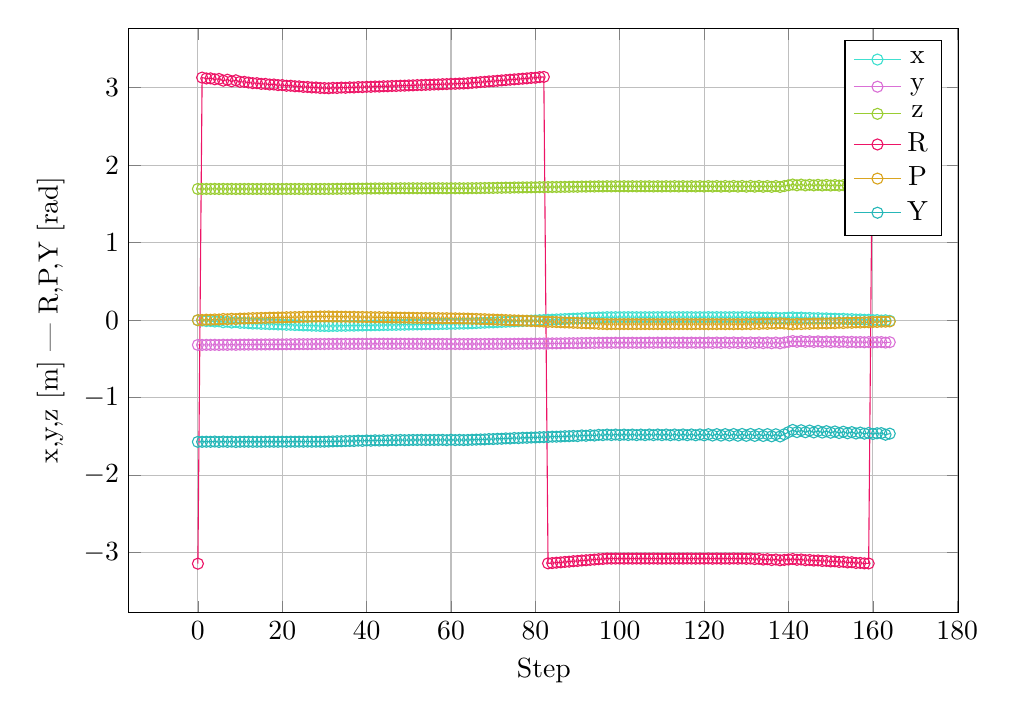
\begin{tikzpicture}
		\begin{axis}[height=9cm, width=\textwidth, grid=major,
		xlabel={Step},ylabel={x,y,z [m] | R,P,Y [rad]}
		]
			\addplot [color=Turquoise, mark=o] coordinates {
				(0, 0.000)
				(1, -0.005)
				(2, -0.011)
				(3, -0.010)
				(4, -0.017)
				(5, -0.014)
				(6, -0.026)
				(7, -0.019)
				(8, -0.030)
				(9, -0.023)
				(10, -0.034)
				(11, -0.034)
				(12, -0.038)
				(13, -0.043)
				(14, -0.043)
				(15, -0.047)
				(16, -0.047)
				(17, -0.051)
				(18, -0.051)
				(19, -0.055)
				(20, -0.055)
				(21, -0.059)
				(22, -0.059)
				(23, -0.063)
				(24, -0.063)
				(25, -0.067)
				(26, -0.067)
				(27, -0.070)
				(28, -0.071)
				(29, -0.074)
				(30, -0.074)
				(31, -0.076)
				(32, -0.073)
				(33, -0.074)
				(34, -0.071)
				(35, -0.072)
				(36, -0.069)
				(37, -0.070)
				(38, -0.068)
				(39, -0.068)
				(40, -0.066)
				(41, -0.066)
				(42, -0.064)
				(43, -0.064)
				(44, -0.062)
				(45, -0.062)
				(46, -0.060)
				(47, -0.060)
				(48, -0.058)
				(49, -0.058)
				(50, -0.056)
				(51, -0.056)
				(52, -0.054)
				(53, -0.054)
				(54, -0.052)
				(55, -0.052)
				(56, -0.050)
				(57, -0.050)
				(58, -0.048)
				(59, -0.048)
				(60, -0.046)
				(61, -0.046)
				(62, -0.044)
				(63, -0.044)
				(64, -0.042)
				(65, -0.039)
				(66, -0.037)
				(67, -0.034)
				(68, -0.032)
				(69, -0.029)
				(70, -0.028)
				(71, -0.025)
				(72, -0.022)
				(73, -0.020)
				(74, -0.018)
				(75, -0.015)
				(76, -0.013)
				(77, -0.010)
				(78, -0.008)
				(79, -0.005)
				(80, -0.003)
				(81, 0.000)
				(82, 0.002)
				(83, 0.005)
				(84, 0.007)
				(85, 0.010)
				(86, 0.012)
				(87, 0.015)
				(88, 0.017)
				(89, 0.020)
				(90, 0.022)
				(91, 0.025)
				(92, 0.027)
				(93, 0.030)
				(94, 0.032)
				(95, 0.035)
				(96, 0.036)
				(97, 0.039)
				(98, 0.038)
				(99, 0.039)
				(100, 0.039)
				(101, 0.039)
				(102, 0.039)
				(103, 0.039)
				(104, 0.039)
				(105, 0.038)
				(106, 0.039)
				(107, 0.038)
				(108, 0.039)
				(109, 0.039)
				(110, 0.039)
				(111, 0.039)
				(112, 0.039)
				(113, 0.039)
				(114, 0.039)
				(115, 0.039)
				(116, 0.039)
				(117, 0.039)
				(118, 0.038)
				(119, 0.039)
				(120, 0.038)
				(121, 0.040)
				(122, 0.038)
				(123, 0.040)
				(124, 0.038)
				(125, 0.039)
				(126, 0.038)
				(127, 0.040)
				(128, 0.037)
				(129, 0.040)
				(130, 0.037)
				(131, 0.039)
				(132, 0.035)
				(133, 0.037)
				(134, 0.032)
				(135, 0.035)
				(136, 0.029)
				(137, 0.032)
				(138, 0.026)
				(139, 0.030)
				(140, 0.033)
				(141, 0.037)
				(142, 0.031)
				(143, 0.034)
				(144, 0.028)
				(145, 0.030)
				(146, 0.025)
				(147, 0.027)
				(148, 0.023)
				(149, 0.024)
				(150, 0.020)
				(151, 0.020)
				(152, 0.016)
				(153, 0.018)
				(154, 0.012)
				(155, 0.014)
				(156, 0.009)
				(157, 0.010)
				(158, 0.006)
				(159, 0.006)
				(160, 0.001)
				(161, 0.002)
				(162, -0.004)
				(163, -0.001)
				(164, -0.008)
			};
			\addlegendentry{x}

			\addplot [color=Orchid, mark=o] coordinates {
				(0, -0.319)
				(1, -0.319)
				(2, -0.318)
				(3, -0.318)
				(4, -0.317)
				(5, -0.319)
				(6, -0.316)
				(7, -0.318)
				(8, -0.315)
				(9, -0.318)
				(10, -0.315)
				(11, -0.315)
				(12, -0.315)
				(13, -0.314)
				(14, -0.314)
				(15, -0.313)
				(16, -0.313)
				(17, -0.312)
				(18, -0.312)
				(19, -0.312)
				(20, -0.311)
				(21, -0.311)
				(22, -0.310)
				(23, -0.310)
				(24, -0.309)
				(25, -0.309)
				(26, -0.309)
				(27, -0.308)
				(28, -0.307)
				(29, -0.307)
				(30, -0.307)
				(31, -0.306)
				(32, -0.306)
				(33, -0.305)
				(34, -0.306)
				(35, -0.305)
				(36, -0.306)
				(37, -0.305)
				(38, -0.305)
				(39, -0.305)
				(40, -0.305)
				(41, -0.305)
				(42, -0.304)
				(43, -0.305)
				(44, -0.304)
				(45, -0.305)
				(46, -0.304)
				(47, -0.305)
				(48, -0.304)
				(49, -0.305)
				(50, -0.305)
				(51, -0.305)
				(52, -0.305)
				(53, -0.305)
				(54, -0.306)
				(55, -0.306)
				(56, -0.306)
				(57, -0.306)
				(58, -0.306)
				(59, -0.307)
				(60, -0.306)
				(61, -0.307)
				(62, -0.307)
				(63, -0.308)
				(64, -0.307)
				(65, -0.307)
				(66, -0.307)
				(67, -0.307)
				(68, -0.307)
				(69, -0.306)
				(70, -0.306)
				(71, -0.305)
				(72, -0.306)
				(73, -0.305)
				(74, -0.305)
				(75, -0.304)
				(76, -0.304)
				(77, -0.303)
				(78, -0.303)
				(79, -0.302)
				(80, -0.302)
				(81, -0.301)
				(82, -0.301)
				(83, -0.301)
				(84, -0.299)
				(85, -0.299)
				(86, -0.299)
				(87, -0.298)
				(88, -0.297)
				(89, -0.296)
				(90, -0.297)
				(91, -0.294)
				(92, -0.295)
				(93, -0.292)
				(94, -0.294)
				(95, -0.291)
				(96, -0.292)
				(97, -0.290)
				(98, -0.292)
				(99, -0.290)
				(100, -0.292)
				(101, -0.290)
				(102, -0.292)
				(103, -0.290)
				(104, -0.292)
				(105, -0.290)
				(106, -0.292)
				(107, -0.289)
				(108, -0.292)
				(109, -0.289)
				(110, -0.292)
				(111, -0.289)
				(112, -0.292)
				(113, -0.289)
				(114, -0.292)
				(115, -0.289)
				(116, -0.292)
				(117, -0.289)
				(118, -0.292)
				(119, -0.289)
				(120, -0.293)
				(121, -0.288)
				(122, -0.293)
				(123, -0.288)
				(124, -0.294)
				(125, -0.287)
				(126, -0.294)
				(127, -0.287)
				(128, -0.294)
				(129, -0.287)
				(130, -0.295)
				(131, -0.287)
				(132, -0.295)
				(133, -0.287)
				(134, -0.296)
				(135, -0.288)
				(136, -0.297)
				(137, -0.288)
				(138, -0.298)
				(139, -0.288)
				(140, -0.279)
				(141, -0.269)
				(142, -0.279)
				(143, -0.270)
				(144, -0.279)
				(145, -0.272)
				(146, -0.280)
				(147, -0.273)
				(148, -0.281)
				(149, -0.275)
				(150, -0.282)
				(151, -0.276)
				(152, -0.283)
				(153, -0.277)
				(154, -0.284)
				(155, -0.279)
				(156, -0.284)
				(157, -0.281)
				(158, -0.285)
				(159, -0.282)
				(160, -0.286)
				(161, -0.283)
				(162, -0.282)
				(163, -0.289)
				(164, -0.284)
			};
			\addlegendentry{y}

			\addplot [color=YellowGreen, mark=o] coordinates {
				(0, 1.694)
				(1, 1.694)
				(2, 1.694)
				(3, 1.694)
				(4, 1.695)
				(5, 1.693)
				(6, 1.695)
				(7, 1.693)
				(8, 1.695)
				(9, 1.693)
				(10, 1.694)
				(11, 1.694)
				(12, 1.694)
				(13, 1.694)
				(14, 1.694)
				(15, 1.694)
				(16, 1.694)
				(17, 1.694)
				(18, 1.694)
				(19, 1.693)
				(20, 1.694)
				(21, 1.694)
				(22, 1.694)
				(23, 1.694)
				(24, 1.694)
				(25, 1.694)
				(26, 1.694)
				(27, 1.694)
				(28, 1.694)
				(29, 1.694)
				(30, 1.694)
				(31, 1.694)
				(32, 1.695)
				(33, 1.696)
				(34, 1.696)
				(35, 1.697)
				(36, 1.697)
				(37, 1.697)
				(38, 1.699)
				(39, 1.698)
				(40, 1.700)
				(41, 1.699)
				(42, 1.701)
				(43, 1.700)
				(44, 1.701)
				(45, 1.700)
				(46, 1.702)
				(47, 1.701)
				(48, 1.703)
				(49, 1.702)
				(50, 1.702)
				(51, 1.703)
				(52, 1.702)
				(53, 1.703)
				(54, 1.702)
				(55, 1.703)
				(56, 1.703)
				(57, 1.703)
				(58, 1.703)
				(59, 1.702)
				(60, 1.704)
				(61, 1.702)
				(62, 1.703)
				(63, 1.702)
				(64, 1.703)
				(65, 1.704)
				(66, 1.704)
				(67, 1.705)
				(68, 1.706)
				(69, 1.707)
				(70, 1.707)
				(71, 1.709)
				(72, 1.709)
				(73, 1.711)
				(74, 1.710)
				(75, 1.713)
				(76, 1.712)
				(77, 1.714)
				(78, 1.714)
				(79, 1.715)
				(80, 1.715)
				(81, 1.717)
				(82, 1.717)
				(83, 1.718)
				(84, 1.719)
				(85, 1.719)
				(86, 1.720)
				(87, 1.721)
				(88, 1.721)
				(89, 1.723)
				(90, 1.722)
				(91, 1.725)
				(92, 1.724)
				(93, 1.727)
				(94, 1.725)
				(95, 1.728)
				(96, 1.726)
				(97, 1.729)
				(98, 1.727)
				(99, 1.729)
				(100, 1.727)
				(101, 1.729)
				(102, 1.727)
				(103, 1.729)
				(104, 1.727)
				(105, 1.729)
				(106, 1.727)
				(107, 1.729)
				(108, 1.726)
				(109, 1.729)
				(110, 1.726)
				(111, 1.729)
				(112, 1.726)
				(113, 1.730)
				(114, 1.726)
				(115, 1.730)
				(116, 1.726)
				(117, 1.730)
				(118, 1.726)
				(119, 1.730)
				(120, 1.725)
				(121, 1.731)
				(122, 1.725)
				(123, 1.731)
				(124, 1.724)
				(125, 1.731)
				(126, 1.724)
				(127, 1.732)
				(128, 1.724)
				(129, 1.732)
				(130, 1.723)
				(131, 1.732)
				(132, 1.723)
				(133, 1.732)
				(134, 1.722)
				(135, 1.731)
				(136, 1.721)
				(137, 1.731)
				(138, 1.720)
				(139, 1.731)
				(140, 1.741)
				(141, 1.751)
				(142, 1.741)
				(143, 1.750)
				(144, 1.740)
				(145, 1.748)
				(146, 1.740)
				(147, 1.747)
				(148, 1.739)
				(149, 1.746)
				(150, 1.738)
				(151, 1.744)
				(152, 1.737)
				(153, 1.743)
				(154, 1.736)
				(155, 1.741)
				(156, 1.735)
				(157, 1.739)
				(158, 1.734)
				(159, 1.737)
				(160, 1.732)
				(161, 1.735)
				(162, 1.736)
				(163, 1.729)
				(164, 1.734)
			};
			\addlegendentry{z}

			\addplot [color=WildStrawberry, mark=o] coordinates {
				(0, -3.142)
				(1, 3.131)
				(2, 3.120)
				(3, 3.121)
				(4, 3.109)
				(5, 3.114)
				(6, 3.091)
				(7, 3.104)
				(8, 3.083)
				(9, 3.096)
				(10, 3.076)
				(11, 3.076)
				(12, 3.067)
				(13, 3.059)
				(14, 3.059)
				(15, 3.050)
				(16, 3.050)
				(17, 3.042)
				(18, 3.042)
				(19, 3.034)
				(20, 3.034)
				(21, 3.026)
				(22, 3.026)
				(23, 3.019)
				(24, 3.018)
				(25, 3.011)
				(26, 3.010)
				(27, 3.004)
				(28, 3.003)
				(29, 2.997)
				(30, 2.996)
				(31, 2.993)
				(32, 2.999)
				(33, 2.997)
				(34, 3.002)
				(35, 3.000)
				(36, 3.005)
				(37, 3.004)
				(38, 3.009)
				(39, 3.008)
				(40, 3.012)
				(41, 3.012)
				(42, 3.016)
				(43, 3.015)
				(44, 3.019)
				(45, 3.019)
				(46, 3.023)
				(47, 3.023)
				(48, 3.026)
				(49, 3.027)
				(50, 3.030)
				(51, 3.031)
				(52, 3.034)
				(53, 3.035)
				(54, 3.038)
				(55, 3.039)
				(56, 3.042)
				(57, 3.043)
				(58, 3.046)
				(59, 3.047)
				(60, 3.050)
				(61, 3.051)
				(62, 3.054)
				(63, 3.055)
				(64, 3.058)
				(65, 3.064)
				(66, 3.067)
				(67, 3.073)
				(68, 3.076)
				(69, 3.082)
				(70, 3.085)
				(71, 3.090)
				(72, 3.095)
				(73, 3.099)
				(74, 3.104)
				(75, 3.108)
				(76, 3.112)
				(77, 3.117)
				(78, 3.121)
				(79, 3.127)
				(80, 3.129)
				(81, 3.137)
				(82, 3.140)
				(83, -3.138)
				(84, -3.134)
				(85, -3.129)
				(86, -3.125)
				(87, -3.119)
				(88, -3.116)
				(89, -3.110)
				(90, -3.107)
				(91, -3.101)
				(92, -3.098)
				(93, -3.093)
				(94, -3.089)
				(95, -3.084)
				(96, -3.081)
				(97, -3.076)
				(98, -3.077)
				(99, -3.076)
				(100, -3.076)
				(101, -3.077)
				(102, -3.076)
				(103, -3.077)
				(104, -3.076)
				(105, -3.077)
				(106, -3.076)
				(107, -3.077)
				(108, -3.076)
				(109, -3.077)
				(110, -3.077)
				(111, -3.077)
				(112, -3.076)
				(113, -3.077)
				(114, -3.076)
				(115, -3.077)
				(116, -3.076)
				(117, -3.076)
				(118, -3.077)
				(119, -3.076)
				(120, -3.077)
				(121, -3.075)
				(122, -3.078)
				(123, -3.075)
				(124, -3.078)
				(125, -3.076)
				(126, -3.078)
				(127, -3.075)
				(128, -3.078)
				(129, -3.075)
				(130, -3.079)
				(131, -3.076)
				(132, -3.083)
				(133, -3.079)
				(134, -3.089)
				(135, -3.084)
				(136, -3.095)
				(137, -3.088)
				(138, -3.099)
				(139, -3.093)
				(140, -3.088)
				(141, -3.082)
				(142, -3.092)
				(143, -3.088)
				(144, -3.097)
				(145, -3.094)
				(146, -3.102)
				(147, -3.100)
				(148, -3.107)
				(149, -3.106)
				(150, -3.113)
				(151, -3.112)
				(152, -3.120)
				(153, -3.117)
				(154, -3.126)
				(155, -3.123)
				(156, -3.133)
				(157, -3.132)
				(158, -3.138)
				(159, -3.139)
				(160, 3.137)
				(161, 3.138)
				(162, 3.125)
				(163, 3.133)
				(164, 3.118)
			};
			\addlegendentry{R}

			\addplot [color=Goldenrod, mark=o] coordinates {
				(0, -0.000)
				(1, 0.003)
				(2, 0.007)
				(3, 0.006)
				(4, 0.010)
				(5, 0.009)
				(6, 0.016)
				(7, 0.012)
				(8, 0.019)
				(9, 0.015)
				(10, 0.021)
				(11, 0.021)
				(12, 0.024)
				(13, 0.027)
				(14, 0.027)
				(15, 0.030)
				(16, 0.030)
				(17, 0.033)
				(18, 0.033)
				(19, 0.035)
				(20, 0.035)
				(21, 0.038)
				(22, 0.038)
				(23, 0.040)
				(24, 0.040)
				(25, 0.043)
				(26, 0.043)
				(27, 0.045)
				(28, 0.046)
				(29, 0.048)
				(30, 0.048)
				(31, 0.049)
				(32, 0.046)
				(33, 0.047)
				(34, 0.045)
				(35, 0.045)
				(36, 0.043)
				(37, 0.044)
				(38, 0.041)
				(39, 0.042)
				(40, 0.040)
				(41, 0.040)
				(42, 0.038)
				(43, 0.039)
				(44, 0.036)
				(45, 0.037)
				(46, 0.034)
				(47, 0.035)
				(48, 0.033)
				(49, 0.033)
				(50, 0.032)
				(51, 0.031)
				(52, 0.030)
				(53, 0.029)
				(54, 0.029)
				(55, 0.028)
				(56, 0.027)
				(57, 0.027)
				(58, 0.025)
				(59, 0.026)
				(60, 0.024)
				(61, 0.024)
				(62, 0.022)
				(63, 0.022)
				(64, 0.021)
				(65, 0.018)
				(66, 0.017)
				(67, 0.014)
				(68, 0.013)
				(69, 0.010)
				(70, 0.009)
				(71, 0.006)
				(72, 0.005)
				(73, 0.002)
				(74, 0.000)
				(75, -0.002)
				(76, -0.004)
				(77, -0.006)
				(78, -0.008)
				(79, -0.011)
				(80, -0.012)
				(81, -0.015)
				(82, -0.017)
				(83, -0.020)
				(84, -0.021)
				(85, -0.024)
				(86, -0.026)
				(87, -0.029)
				(88, -0.030)
				(89, -0.033)
				(90, -0.034)
				(91, -0.038)
				(92, -0.039)
				(93, -0.042)
				(94, -0.043)
				(95, -0.047)
				(96, -0.048)
				(97, -0.051)
				(98, -0.050)
				(99, -0.050)
				(100, -0.050)
				(101, -0.050)
				(102, -0.050)
				(103, -0.050)
				(104, -0.050)
				(105, -0.050)
				(106, -0.050)
				(107, -0.050)
				(108, -0.050)
				(109, -0.050)
				(110, -0.050)
				(111, -0.050)
				(112, -0.050)
				(113, -0.050)
				(114, -0.050)
				(115, -0.050)
				(116, -0.050)
				(117, -0.051)
				(118, -0.050)
				(119, -0.050)
				(120, -0.050)
				(121, -0.051)
				(122, -0.049)
				(123, -0.051)
				(124, -0.049)
				(125, -0.051)
				(126, -0.049)
				(127, -0.052)
				(128, -0.049)
				(129, -0.052)
				(130, -0.048)
				(131, -0.051)
				(132, -0.046)
				(133, -0.050)
				(134, -0.043)
				(135, -0.047)
				(136, -0.041)
				(137, -0.045)
				(138, -0.038)
				(139, -0.043)
				(140, -0.048)
				(141, -0.053)
				(142, -0.046)
				(143, -0.050)
				(144, -0.044)
				(145, -0.047)
				(146, -0.041)
				(147, -0.044)
				(148, -0.039)
				(149, -0.042)
				(150, -0.037)
				(151, -0.039)
				(152, -0.033)
				(153, -0.037)
				(154, -0.031)
				(155, -0.033)
				(156, -0.028)
				(157, -0.030)
				(158, -0.026)
				(159, -0.026)
				(160, -0.022)
				(161, -0.023)
				(162, -0.019)
				(163, -0.019)
				(164, -0.016)
			};
			\addlegendentry{P}

			\addplot [color=BlueGreen, mark=o] coordinates {
				(0, -1.570)
				(1, -1.569)
				(2, -1.568)
				(3, -1.569)
				(4, -1.566)
				(5, -1.571)
				(6, -1.566)
				(7, -1.570)
				(8, -1.567)
				(9, -1.572)
				(10, -1.568)
				(11, -1.568)
				(12, -1.568)
				(13, -1.569)
				(14, -1.569)
				(15, -1.569)
				(16, -1.568)
				(17, -1.568)
				(18, -1.568)
				(19, -1.569)
				(20, -1.567)
				(21, -1.569)
				(22, -1.567)
				(23, -1.568)
				(24, -1.567)
				(25, -1.568)
				(26, -1.567)
				(27, -1.568)
				(28, -1.567)
				(29, -1.568)
				(30, -1.567)
				(31, -1.566)
				(32, -1.564)
				(33, -1.562)
				(34, -1.562)
				(35, -1.560)
				(36, -1.559)
				(37, -1.559)
				(38, -1.554)
				(39, -1.557)
				(40, -1.552)
				(41, -1.555)
				(42, -1.550)
				(43, -1.553)
				(44, -1.549)
				(45, -1.552)
				(46, -1.546)
				(47, -1.550)
				(48, -1.545)
				(49, -1.548)
				(50, -1.547)
				(51, -1.545)
				(52, -1.546)
				(53, -1.544)
				(54, -1.546)
				(55, -1.545)
				(56, -1.545)
				(57, -1.545)
				(58, -1.544)
				(59, -1.548)
				(60, -1.542)
				(61, -1.547)
				(62, -1.544)
				(63, -1.547)
				(64, -1.545)
				(65, -1.543)
				(66, -1.541)
				(67, -1.539)
				(68, -1.538)
				(69, -1.534)
				(70, -1.534)
				(71, -1.530)
				(72, -1.530)
				(73, -1.525)
				(74, -1.526)
				(75, -1.520)
				(76, -1.522)
				(77, -1.517)
				(78, -1.517)
				(79, -1.514)
				(80, -1.513)
				(81, -1.510)
				(82, -1.509)
				(83, -1.507)
				(84, -1.503)
				(85, -1.503)
				(86, -1.501)
				(87, -1.497)
				(88, -1.497)
				(89, -1.493)
				(90, -1.496)
				(91, -1.487)
				(92, -1.491)
				(93, -1.483)
				(94, -1.488)
				(95, -1.479)
				(96, -1.483)
				(97, -1.476)
				(98, -1.482)
				(99, -1.476)
				(100, -1.482)
				(101, -1.476)
				(102, -1.482)
				(103, -1.476)
				(104, -1.483)
				(105, -1.476)
				(106, -1.483)
				(107, -1.475)
				(108, -1.483)
				(109, -1.475)
				(110, -1.483)
				(111, -1.475)
				(112, -1.484)
				(113, -1.475)
				(114, -1.484)
				(115, -1.474)
				(116, -1.484)
				(117, -1.474)
				(118, -1.485)
				(119, -1.474)
				(120, -1.486)
				(121, -1.471)
				(122, -1.488)
				(123, -1.470)
				(124, -1.489)
				(125, -1.470)
				(126, -1.489)
				(127, -1.469)
				(128, -1.491)
				(129, -1.468)
				(130, -1.492)
				(131, -1.468)
				(132, -1.493)
				(133, -1.469)
				(134, -1.494)
				(135, -1.470)
				(136, -1.498)
				(137, -1.472)
				(138, -1.500)
				(139, -1.472)
				(140, -1.444)
				(141, -1.416)
				(142, -1.444)
				(143, -1.420)
				(144, -1.446)
				(145, -1.424)
				(146, -1.448)
				(147, -1.428)
				(148, -1.450)
				(149, -1.432)
				(150, -1.452)
				(151, -1.436)
				(152, -1.456)
				(153, -1.439)
				(154, -1.459)
				(155, -1.444)
				(156, -1.462)
				(157, -1.450)
				(158, -1.464)
				(159, -1.455)
				(160, -1.468)
				(161, -1.459)
				(162, -1.457)
				(163, -1.478)
				(164, -1.464)
			};
			\addlegendentry{Y}

		\end{axis}
	\end{tikzpicture}
	\caption{Robot camera's frame while tracking the marker at medium speed.}
	\label{fig:cameraPoseCornyMediumPlot}
\end{figure}
}

\providecommand{\errorCornyPlot}{
\begin{figure}[!ht]
	\centering
	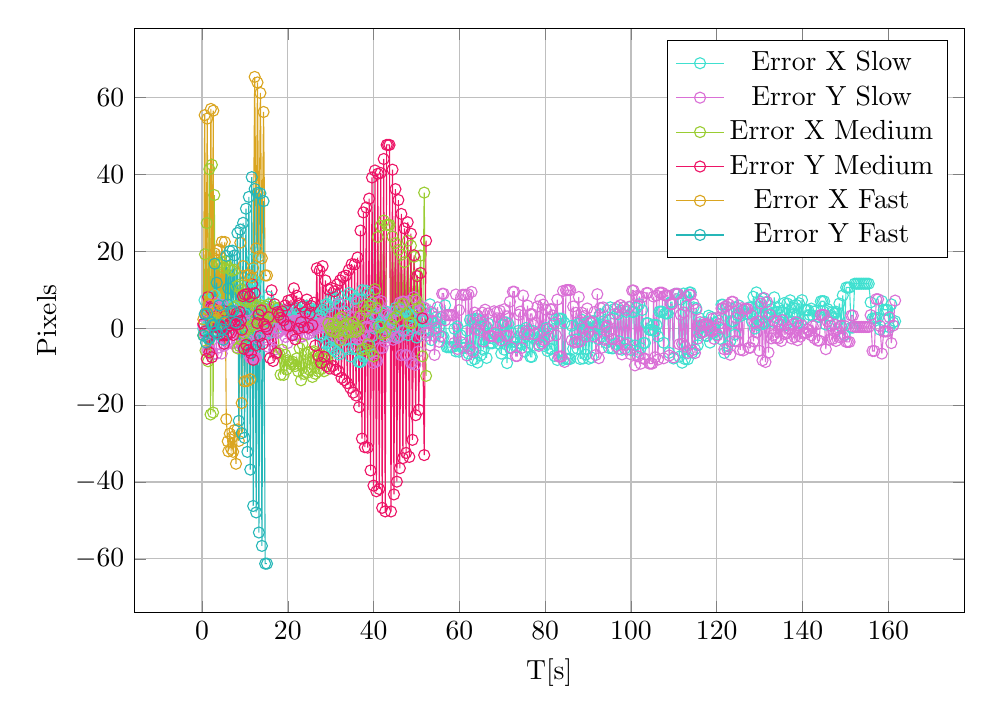
\begin{tikzpicture}
		\begin{axis}[height=9cm, width=\textwidth, grid=major,
		xlabel={T[s]},ylabel={Pixels}
		]
			\addplot [color=Turquoise, mark=o] coordinates {
				(0.294,-0.154)
				(0.580,7.291)
				(0.837,-1.147)
				(1.138,5.432)
				(1.457,0.926)
				(1.743,0.926)
				(1.843,0.926)
				(2.138,5.183)
				(2.434,-1.098)
				(2.747,8.532)
				(3.049,8.532)
				(3.358,-0.605)
				(3.669,6.386)
				(3.981,-0.345)
				(4.286,5.284)
				(4.600,1.106)
				(4.896,4.886)
				(5.202,0.926)
				(5.505,4.806)
				(5.805,0.841)
				(5.899,4.837)
				(6.043,0.935)
				(6.353,5.516)
				(6.642,0.060)
				(6.943,5.720)
				(7.241,5.720)
				(7.531,5.720)
				(7.809,0.846)
				(8.090,4.382)
				(8.371,3.163)
				(8.650,1.219)
				(8.944,4.827)
				(9.220,0.864)
				(9.490,0.864)
				(9.772,0.864)
				(10.004,3.616)
				(10.294,8.713)
				(10.577,-2.587)
				(10.717,7.603)
				(10.974,-1.116)
				(11.248,12.173)
				(11.509,12.173)
				(11.752,17.934)
				(12.032,12.173)
				(12.295,12.173)
				(12.565,12.173)
				(12.859,-4.200)
				(13.149,7.147)
				(13.420,1.088)
				(13.715,4.080)
				(13.999,3.314)
				(14.283,1.226)
				(14.571,3.179)
				(14.856,5.041)
				(15.141,-1.160)
				(15.423,8.190)
				(15.697,-1.377)
				(15.973,6.437)
				(16.246,0.508)
				(16.544,4.513)
				(16.825,3.024)
				(17.078,3.024)
				(17.346,4.860)
				(17.607,0.173)
				(17.880,5.141)
				(18.132,1.570)
				(18.379,4.814)
				(18.635,1.712)
				(18.892,3.428)
				(19.165,3.428)
				(19.431,3.260)
				(19.689,1.822)
				(19.934,4.238)
				(20.202,2.780)
				(20.457,3.936)
				(20.719,1.782)
				(20.982,4.557)
				(21.224,0.671)
				(21.480,0.671)
				(21.761,5.331)
				(22.037,1.413)
				(22.312,4.822)
				(22.586,1.795)
				(22.856,4.553)
				(23.103,1.547)
				(23.380,5.400)
				(23.652,0.493)
				(23.931,5.800)
				(24.199,0.578)
				(24.469,5.773)
				(24.743,0.808)
				(25.005,5.409)
				(25.271,1.121)
				(25.537,5.069)
				(25.801,1.832)
				(26.056,4.578)
				(26.307,1.537)
				(26.567,4.618)
				(26.823,3.333)
				(27.067,-1.516)
				(27.323,3.201)
				(27.570,3.201)
				(27.850,-1.892)
				(28.113,4.778)
				(28.373,-3.655)
				(28.624,6.071)
				(28.872,-4.127)
				(29.130,6.209)
				(29.386,-3.693)
				(29.649,5.575)
				(29.898,-4.916)
				(30.143,8.000)
				(30.390,-5.375)
				(30.638,7.374)
				(30.892,-5.748)
				(31.155,7.822)
				(31.405,-6.281)
				(31.677,8.539)
				(31.925,-6.831)
				(32.178,6.361)
				(32.420,0.241)
				(32.666,1.549)
				(32.931,-0.061)
				(33.195,4.320)
				(33.468,-3.068)
				(33.749,6.101)
				(34.030,-5.442)
				(34.319,9.149)
				(34.614,-7.376)
				(34.922,8.674)
				(35.224,-5.443)
				(35.513,7.622)
				(35.818,-5.379)
				(36.136,7.709)
				(36.436,-8.749)
				(36.748,-8.749)
				(37.058,-8.749)
				(37.361,9.882)
				(37.646,-7.366)
				(37.954,-7.366)
				(38.236,9.744)
				(38.521,-7.115)
				(38.812,8.959)
				(39.092,-4.465)
				(39.386,5.764)
				(39.662,-2.126)
				(39.952,3.525)
				(40.258,-0.139)
				(40.556,2.830)
				(40.860,2.830)
				(41.167,0.456)
				(41.474,0.940)
				(41.782,1.472)
				(42.077,0.681)
				(42.372,3.790)
				(42.680,-2.137)
				(42.997,4.298)
				(43.302,-0.438)
				(43.615,1.116)
				(43.928,2.505)
				(44.246,-0.495)
				(44.546,4.320)
				(44.864,-2.230)
				(45.179,5.298)
				(45.483,-2.533)
				(45.809,4.546)
				(46.120,-2.057)
				(46.435,4.877)
				(46.749,-0.639)
				(47.070,-0.639)
				(47.373,4.378)
				(47.694,4.378)
				(48.033,-1.814)
				(48.367,3.219)
				(48.698,3.155)
				(49.040,3.155)
				(49.377,0.159)
				(49.716,3.520)
				(50.063,-2.453)
				(50.399,4.477)
				(50.756,-0.285)
				(51.084,1.951)
				(51.427,1.751)
				(51.770,1.751)
				(52.113,1.895)
				(52.459,0.063)
				(52.812,-0.237)
				(53.151,6.204)
				(53.506,-3.094)
				(53.861,3.746)
				(54.211,-0.191)
				(54.566,2.799)
				(54.920,1.617)
				(55.277,0.333)
				(55.633,2.886)
				(55.978,-2.269)
				(56.325,-2.269)
				(56.673,5.955)
				(57.024,-4.948)
				(57.382,-4.948)
				(57.747,-4.948)
				(58.112,-4.948)
				(58.475,-4.948)
				(58.831,-0.170)
				(59.184,-6.047)
				(59.549,0.448)
				(59.932,-6.139)
				(60.299,-1.855)
				(60.657,-5.098)
				(61.024,-5.098)
				(61.389,-5.098)
				(61.755,-0.681)
				(62.113,-6.614)
				(62.480,2.169)
				(62.837,-8.332)
				(63.201,2.310)
				(63.559,-8.047)
				(63.905,2.483)
				(64.252,-8.960)
				(64.606,2.149)
				(64.945,-7.098)
				(65.305,0.043)
				(65.646,-5.604)
				(65.994,0.577)
				(66.342,-7.748)
				(66.683,1.221)
				(67.034,-3.931)
				(67.386,-3.931)
				(67.734,-3.931)
				(68.083,-2.800)
				(68.423,-1.584)
				(68.763,-2.469)
				(69.090,-4.009)
				(69.431,-1.618)
				(69.763,-6.614)
				(70.109,0.784)
				(70.442,-5.585)
				(70.777,1.508)
				(71.112,-9.094)
				(71.451,1.084)
				(71.785,-5.212)
				(72.128,-1.181)
				(72.462,-3.522)
				(72.797,-3.522)
				(73.144,-4.954)
				(73.485,-4.954)
				(73.836,-0.645)
				(74.178,-3.814)
				(74.513,-4.199)
				(74.858,-0.743)
				(75.198,-6.099)
				(75.543,0.055)
				(75.886,-4.786)
				(76.217,-0.501)
				(76.551,-7.467)
				(76.890,-7.467)
				(77.198,-0.726)
				(77.531,-4.554)
				(77.874,-2.680)
				(78.219,-1.592)
				(78.535,-4.257)
				(78.859,-2.044)
				(79.194,-3.431)
				(79.526,-2.026)
				(79.846,-4.656)
				(80.188,0.043)
				(80.520,-5.914)
				(80.841,-0.243)
				(81.173,-5.415)
				(81.498,-5.415)
				(81.841,0.992)
				(82.173,-7.234)
				(82.508,2.325)
				(82.832,-8.280)
				(83.158,2.464)
				(83.500,2.464)
				(83.843,2.464)
				(84.168,-8.255)
				(84.511,1.348)
				(84.849,-8.021)
				(85.173,-8.021)
				(85.500,-8.021)
				(85.837,-8.021)
				(86.177,0.612)
				(86.524,-5.367)
				(86.856,-1.428)
				(87.177,-2.954)
				(87.506,-5.310)
				(87.843,1.166)
				(88.169,-8.015)
				(88.502,2.226)
				(88.827,-7.889)
				(89.152,0.974)
				(89.476,-6.897)
				(89.805,1.413)
				(90.151,-7.967)
				(90.496,1.837)
				(90.835,-7.631)
				(91.166,1.797)
				(91.501,-1.448)
				(91.827,0.431)
				(92.162,0.768)
				(92.501,-2.912)
				(92.839,3.622)
				(93.186,-2.240)
				(93.519,1.774)
				(93.862,0.698)
				(94.190,-3.787)
				(94.517,4.668)
				(94.866,-5.143)
				(95.190,5.418)
				(95.534,-5.245)
				(95.868,-5.245)
				(96.217,5.051)
				(96.555,-4.087)
				(96.899,3.618)
				(97.239,-3.417)
				(97.578,4.598)
				(97.918,-5.609)
				(98.259,5.379)
				(98.583,-5.317)
				(98.927,4.205)
				(99.262,-3.852)
				(99.601,5.466)
				(99.934,-5.654)
				(100.274,4.192)
				(100.605,4.192)
				(100.938,-4.470)
				(101.273,5.264)
				(101.605,-6.155)
				(101.938,6.203)
				(102.276,-5.188)
				(102.610,4.697)
				(102.941,-3.852)
				(103.277,-3.852)
				(103.609,1.306)
				(103.951,1.306)
				(104.289,-0.456)
				(104.634,-0.456)
				(104.971,-0.456)
				(105.296,0.869)
				(105.636,-0.805)
				(105.964,0.799)
				(106.299,-2.195)
				(106.624,4.292)
				(106.954,4.292)
				(107.287,4.292)
				(107.623,-3.792)
				(107.955,3.833)
				(108.279,3.833)
				(108.601,3.833)
				(108.933,-6.394)
				(109.265,6.767)
				(109.591,6.767)
				(109.919,-7.910)
				(110.257,8.911)
				(110.603,8.911)
				(110.941,8.911)
				(111.271,-7.407)
				(111.600,7.422)
				(111.928,-8.987)
				(112.256,9.000)
				(112.600,-8.056)
				(112.926,8.218)
				(113.267,-8.091)
				(113.594,9.273)
				(113.930,9.273)
				(114.258,-6.351)
				(114.586,5.405)
				(114.929,-5.500)
				(115.223,5.211)
				(115.565,-4.438)
				(115.894,2.639)
				(116.099,-1.269)
				(116.435,0.811)
				(116.765,-0.990)
				(117.102,1.595)
				(117.431,-2.017)
				(117.772,-2.017)
				(118.103,3.248)
				(118.433,-3.755)
				(118.770,2.862)
				(119.095,-1.280)
				(119.420,-0.225)
				(119.764,1.389)
				(120.095,-1.645)
				(120.434,1.921)
				(120.767,-2.795)
				(121.104,6.097)
				(121.431,6.097)
				(121.771,-6.449)
				(122.118,5.626)
				(122.463,-4.672)
				(122.799,4.434)
				(123.141,-3.477)
				(123.477,1.749)
				(123.809,1.749)
				(124.164,-1.695)
				(124.497,5.356)
				(124.821,3.398)
				(125.150,5.895)
				(125.485,3.099)
				(125.825,4.490)
				(126.154,4.665)
				(126.491,3.679)
				(126.826,3.679)
				(127.155,3.679)
				(127.495,5.366)
				(127.847,5.366)
				(128.192,1.719)
				(128.545,8.158)
				(128.897,-0.105)
				(129.254,9.304)
				(129.613,0.806)
				(129.960,7.006)
				(130.306,0.966)
				(130.656,7.724)
				(131.006,1.172)
				(131.357,6.675)
				(131.717,3.558)
				(132.058,4.259)
				(132.401,3.662)
				(132.734,4.968)
				(133.068,1.716)
				(133.411,8.017)
				(133.745,2.747)
				(134.067,4.189)
				(134.362,5.257)
				(134.701,3.363)
				(135.039,4.422)
				(135.371,4.095)
				(135.718,6.529)
				(136.069,0.731)
				(136.422,6.409)
				(136.769,1.551)
				(137.117,7.242)
				(137.467,1.794)
				(137.822,5.283)
				(138.164,3.730)
				(138.499,6.052)
				(138.840,1.352)
				(139.176,6.491)
				(139.522,1.299)
				(139.869,7.294)
				(140.224,2.248)
				(140.582,4.686)
				(140.944,4.686)
				(141.307,4.718)
				(141.674,3.436)
				(142.033,5.090)
				(142.402,3.249)
				(142.770,4.313)
				(143.149,4.470)
				(143.515,2.936)
				(143.896,2.936)
				(144.269,6.997)
				(144.655,6.997)
				(145.040,6.997)
				(145.432,0.922)
				(145.831,4.975)
				(146.217,4.210)
				(146.622,3.171)
				(147.009,4.142)
				(147.408,3.797)
				(147.798,4.283)
				(148.198,1.689)
				(148.593,6.402)
				(148.990,0.498)
				(149.384,8.527)
				(149.771,-1.769)
				(150.172,10.566)
				(150.565,10.566)
				(150.957,10.566)
				(151.342,0.148)
				(151.738,0.148)
				(152.143,11.562)
				(152.554,11.562)
				(152.955,11.562)
				(153.359,11.562)
				(153.770,11.562)
				(154.182,11.562)
				(154.594,11.562)
				(155.014,11.562)
				(155.435,11.562)
				(155.871,6.722)
				(156.311,2.498)
				(156.755,2.498)
				(157.179,2.664)
				(157.615,2.664)
				(158.050,-0.398)
				(158.491,7.052)
				(158.927,4.772)
				(159.364,4.772)
				(159.828,4.772)
				(160.264,0.189)
				(160.702,6.190)
				(161.146,1.471)
				(161.584,1.798)

			};
			\addlegendentry{Error X Slow}

			\addplot [color=Orchid, mark=o] coordinates {
				(0.294,0.661)
				(0.580,-1.343)
				(0.837,-1.814)
				(1.138,4.397)
				(1.457,-5.659)
				(1.743,-5.659)
				(1.843,-5.659)
				(2.138,5.902)
				(2.434,-6.901)
				(2.747,6.530)
				(3.049,6.530)
				(3.358,-6.665)
				(3.669,5.555)
				(3.981,-5.039)
				(4.286,5.767)
				(4.600,-6.605)
				(4.896,5.978)
				(5.202,-4.532)
				(5.505,3.771)
				(5.805,-3.203)
				(5.899,3.750)
				(6.043,-3.879)
				(6.353,-0.465)
				(6.642,4.200)
				(6.943,-3.913)
				(7.241,-3.913)
				(7.531,-3.913)
				(7.809,4.558)
				(8.090,-5.009)
				(8.371,1.524)
				(8.650,0.995)
				(8.944,1.181)
				(9.220,-0.716)
				(9.490,-0.716)
				(9.772,-0.716)
				(10.004,1.664)
				(10.294,-3.391)
				(10.577,4.566)
				(10.717,-3.044)
				(10.974,1.388)
				(11.248,-7.706)
				(11.509,-7.706)
				(11.752,-7.706)
				(12.032,-7.706)
				(12.295,-7.706)
				(12.565,-7.706)
				(12.859,4.802)
				(13.149,-2.802)
				(13.420,0.468)
				(13.715,1.199)
				(13.999,-1.835)
				(14.283,2.203)
				(14.571,0.598)
				(14.856,-2.982)
				(15.141,4.804)
				(15.423,-4.870)
				(15.697,2.312)
				(15.973,0.582)
				(16.246,-2.443)
				(16.544,3.998)
				(16.825,-5.589)
				(17.078,-5.589)
				(17.346,3.441)
				(17.607,-1.251)
				(17.880,-0.966)
				(18.132,2.165)
				(18.379,-0.596)
				(18.635,-0.174)
				(18.892,0.598)
				(19.165,0.598)
				(19.431,-2.268)
				(19.689,4.869)
				(19.934,-3.883)
				(20.202,1.550)
				(20.457,-1.020)
				(20.719,1.370)
				(20.982,-1.563)
				(21.224,1.853)
				(21.480,1.853)
				(21.761,-1.758)
				(22.037,1.744)
				(22.312,-1.310)
				(22.586,1.954)
				(22.856,-2.310)
				(23.103,2.356)
				(23.380,-2.179)
				(23.652,2.139)
				(23.931,-1.685)
				(24.199,1.705)
				(24.469,-1.665)
				(24.743,1.940)
				(25.005,-1.397)
				(25.271,1.008)
				(25.537,-0.561)
				(25.801,0.410)
				(26.056,-0.076)
				(26.307,0.289)
				(26.567,-0.175)
				(26.823,1.996)
				(27.067,0.777)
				(27.323,1.192)
				(27.570,1.192)
				(27.850,0.127)
				(28.113,1.385)
				(28.373,1.210)
				(28.624,0.975)
				(28.872,0.226)
				(29.130,1.709)
				(29.386,0.650)
				(29.649,1.135)
				(29.898,1.166)
				(30.143,0.451)
				(30.390,1.409)
				(30.638,-0.621)
				(30.892,3.819)
				(31.155,-2.079)
				(31.405,1.480)
				(31.677,-1.388)
				(31.925,6.330)
				(32.178,-0.420)
				(32.420,-3.057)
				(32.666,2.626)
				(32.931,1.109)
				(33.195,-1.498)
				(33.468,2.956)
				(33.749,0.429)
				(34.030,-0.969)
				(34.319,3.244)
				(34.614,0.571)
				(34.922,-0.612)
				(35.224,0.658)
				(35.513,2.795)
				(35.818,-4.282)
				(36.136,6.819)
				(36.436,-2.812)
				(36.748,-2.812)
				(37.058,-2.812)
				(37.361,2.475)
				(37.646,-1.906)
				(37.954,-1.906)
				(38.236,0.300)
				(38.521,0.290)
				(38.812,2.625)
				(39.092,-2.018)
				(39.386,0.562)
				(39.662,4.812)
				(39.952,-9.059)
				(40.258,9.348)
				(40.556,-8.563)
				(40.860,-8.563)
				(41.167,6.555)
				(41.474,-5.147)
				(41.782,7.019)
				(42.077,-5.183)
				(42.372,4.309)
				(42.680,-3.545)
				(42.997,3.458)
				(43.302,-2.339)
				(43.615,3.211)
				(43.928,-0.874)
				(44.246,1.387)
				(44.546,-3.009)
				(44.864,0.057)
				(45.179,4.341)
				(45.483,-2.515)
				(45.809,-2.246)
				(46.120,6.642)
				(46.435,-7.019)
				(46.749,6.905)
				(47.070,6.905)
				(47.373,-7.023)
				(47.694,-7.023)
				(48.033,-0.509)
				(48.367,7.109)
				(48.698,-9.038)
				(49.040,-9.038)
				(49.377,8.097)
				(49.716,-9.529)
				(50.063,7.091)
				(50.399,-6.102)
				(50.756,4.550)
				(51.084,-1.919)
				(51.427,5.340)
				(51.770,5.340)
				(52.113,-1.202)
				(52.459,2.280)
				(52.812,-1.095)
				(53.151,-4.481)
				(53.506,4.185)
				(53.861,1.890)
				(54.211,-6.967)
				(54.566,-0.010)
				(54.920,5.428)
				(55.277,-3.545)
				(55.633,-2.126)
				(55.978,8.941)
				(56.325,8.941)
				(56.673,2.026)
				(57.024,3.378)
				(57.382,3.378)
				(57.747,3.378)
				(58.112,3.378)
				(58.475,3.378)
				(58.831,-3.825)
				(59.184,8.743)
				(59.549,-5.406)
				(59.932,4.686)
				(60.299,-3.595)
				(60.657,8.666)
				(61.024,8.666)
				(61.389,8.666)
				(61.755,-7.094)
				(62.113,8.784)
				(62.480,-5.282)
				(62.837,9.419)
				(63.201,-6.150)
				(63.559,4.037)
				(63.905,-0.221)
				(64.252,3.276)
				(64.606,-0.534)
				(64.945,1.063)
				(65.305,4.055)
				(65.646,-3.468)
				(65.994,4.799)
				(66.342,0.349)
				(66.683,3.821)
				(67.034,-2.039)
				(67.386,-2.039)
				(67.734,-2.039)
				(68.083,4.391)
				(68.423,-1.086)
				(68.763,4.152)
				(69.090,-2.487)
				(69.431,4.505)
				(69.763,-3.177)
				(70.109,1.529)
				(70.442,4.902)
				(70.777,-1.967)
				(71.112,3.061)
				(71.451,-1.990)
				(71.785,6.888)
				(72.128,-5.097)
				(72.462,9.469)
				(72.797,9.469)
				(73.144,-7.257)
				(73.485,-7.257)
				(73.836,3.479)
				(74.178,4.283)
				(74.513,-5.168)
				(74.858,8.484)
				(75.198,-1.542)
				(75.543,-0.901)
				(75.886,5.852)
				(76.217,-1.630)
				(76.551,3.665)
				(76.890,3.665)
				(77.198,0.854)
				(77.531,-1.595)
				(77.874,1.442)
				(78.219,5.616)
				(78.535,-4.619)
				(78.859,7.404)
				(79.194,-4.010)
				(79.526,6.099)
				(79.846,-3.162)
				(80.188,4.767)
				(80.520,-0.240)
				(80.841,-2.161)
				(81.173,4.895)
				(81.498,4.895)
				(81.841,3.266)
				(82.173,1.411)
				(82.508,-1.837)
				(82.832,7.411)
				(83.158,-7.397)
				(83.500,-7.397)
				(83.843,-7.397)
				(84.168,9.667)
				(84.511,-8.784)
				(84.849,9.889)
				(85.173,9.889)
				(85.500,9.889)
				(85.837,9.889)
				(86.177,-3.155)
				(86.524,5.623)
				(86.856,-3.717)
				(87.177,3.984)
				(87.506,-3.622)
				(87.843,8.100)
				(88.169,-3.469)
				(88.502,4.026)
				(88.827,-0.081)
				(89.152,3.115)
				(89.476,-2.219)
				(89.805,5.114)
				(90.151,-0.962)
				(90.496,1.484)
				(90.835,1.293)
				(91.166,-2.165)
				(91.501,4.204)
				(91.827,-6.966)
				(92.162,8.827)
				(92.501,-7.804)
				(92.839,5.243)
				(93.186,-5.092)
				(93.519,5.391)
				(93.862,-3.047)
				(94.190,0.070)
				(94.517,0.588)
				(94.866,-0.871)
				(95.190,2.287)
				(95.534,-2.836)
				(95.868,-2.836)
				(96.217,3.673)
				(96.555,-4.660)
				(96.899,5.499)
				(97.239,-5.426)
				(97.578,5.991)
				(97.918,-6.828)
				(98.259,5.444)
				(98.583,-4.196)
				(98.927,4.731)
				(99.262,-5.478)
				(99.601,5.567)
				(99.934,-6.782)
				(100.274,9.787)
				(100.605,9.787)
				(100.938,-9.692)
				(101.273,8.311)
				(101.605,-7.317)
				(101.938,8.265)
				(102.276,-9.239)
				(102.610,8.092)
				(102.941,-7.943)
				(103.277,-7.943)
				(103.609,9.134)
				(103.951,9.134)
				(104.289,-9.218)
				(104.634,-9.218)
				(104.971,-9.218)
				(105.296,8.194)
				(105.636,-7.536)
				(105.964,8.472)
				(106.299,-8.184)
				(106.624,9.215)
				(106.954,9.215)
				(107.287,9.215)
				(107.623,-7.840)
				(107.955,8.467)
				(108.279,8.467)
				(108.601,8.467)
				(108.933,-7.127)
				(109.265,6.237)
				(109.591,6.237)
				(109.919,-7.601)
				(110.257,8.921)
				(110.603,8.921)
				(110.941,8.921)
				(111.271,-4.182)
				(111.600,3.474)
				(111.928,-4.010)
				(112.256,4.098)
				(112.600,-4.817)
				(112.926,5.825)
				(113.267,-6.446)
				(113.594,8.642)
				(113.930,8.642)
				(114.258,-5.741)
				(114.586,6.342)
				(114.929,-6.482)
				(115.223,4.767)
				(115.565,-2.739)
				(115.894,0.496)
				(116.099,1.565)
				(116.435,-1.228)
				(116.765,0.914)
				(117.102,-0.872)
				(117.431,1.056)
				(117.772,1.056)
				(118.103,0.366)
				(118.433,-0.700)
				(118.770,-0.849)
				(119.095,2.511)
				(119.420,-2.788)
				(119.764,2.546)
				(120.095,-1.933)
				(120.434,1.038)
				(120.767,0.139)
				(121.104,5.152)
				(121.431,5.152)
				(121.771,-5.506)
				(122.118,5.697)
				(122.463,-5.432)
				(122.799,6.165)
				(123.141,-6.925)
				(123.477,6.848)
				(123.809,6.848)
				(124.164,-3.354)
				(124.497,2.682)
				(124.821,-3.428)
				(125.150,3.828)
				(125.485,-5.634)
				(125.825,5.189)
				(126.154,-5.802)
				(126.491,5.034)
				(126.826,5.034)
				(127.155,5.034)
				(127.495,-5.092)
				(127.847,-5.092)
				(128.192,3.333)
				(128.545,-3.417)
				(128.897,1.295)
				(129.254,-1.123)
				(129.613,1.831)
				(129.960,-5.866)
				(130.306,6.418)
				(130.656,-8.362)
				(131.006,7.841)
				(131.357,-8.801)
				(131.717,6.814)
				(132.058,-6.339)
				(132.401,3.428)
				(132.734,-2.669)
				(133.068,-1.822)
				(133.411,1.940)
				(133.745,-2.539)
				(134.067,1.735)
				(134.362,-2.721)
				(134.701,1.006)
				(135.039,-3.336)
				(135.371,2.085)
				(135.718,-1.540)
				(136.069,-1.534)
				(136.422,-1.228)
				(136.769,-0.005)
				(137.117,-0.381)
				(137.467,-2.684)
				(137.822,1.015)
				(138.164,-2.331)
				(138.499,1.537)
				(138.840,-3.143)
				(139.176,0.647)
				(139.522,-2.182)
				(139.869,0.710)
				(140.224,-1.382)
				(140.582,-1.184)
				(140.944,-1.184)
				(141.307,-0.331)
				(141.674,-0.773)
				(142.033,-1.862)
				(142.402,0.494)
				(142.770,-2.648)
				(143.149,0.913)
				(143.515,-3.236)
				(143.896,-3.236)
				(144.269,3.453)
				(144.655,3.453)
				(145.040,3.453)
				(145.432,-5.463)
				(145.831,1.765)
				(146.217,-3.042)
				(146.622,0.630)
				(147.009,-2.799)
				(147.408,0.960)
				(147.798,-3.334)
				(148.198,-0.306)
				(148.593,-2.326)
				(148.990,0.677)
				(149.384,-2.273)
				(149.771,0.595)
				(150.172,-3.578)
				(150.565,-3.578)
				(150.957,-3.578)
				(151.342,3.281)
				(151.738,3.281)
				(152.143,0.309)
				(152.554,0.309)
				(152.955,0.309)
				(153.359,0.309)
				(153.770,0.309)
				(154.182,0.309)
				(154.594,0.309)
				(155.014,0.309)
				(155.435,0.309)
				(155.871,3.386)
				(156.311,-5.936)
				(156.755,-5.936)
				(157.179,7.521)
				(157.615,7.521)
				(158.050,0.564)
				(158.491,-6.617)
				(158.927,-0.857)
				(159.364,-0.857)
				(159.828,-0.857)
				(160.264,2.839)
				(160.702,-3.888)
				(161.146,0.674)
				(161.584,7.170)

			};
			\addlegendentry{Error Y Slow}

			\addplot [color=YellowGreen, mark=o] coordinates {
				(0.308,-1.843)
				(0.407,-1.843)
				(0.702,19.194)
				(0.805,-5.838)
				(1.105,27.316)
				(1.414,-8.603)
				(1.707,41.346)
				(2.001,-22.455)
				(2.296,42.492)
				(2.579,-21.932)
				(2.857,34.606)
				(3.116,1.639)
				(3.387,1.639)
				(3.658,16.853)
				(3.895,1.487)
				(4.148,16.546)
				(4.379,1.800)
				(4.631,17.105)
				(4.832,2.924)
				(5.089,15.702)
				(5.149,2.322)
				(5.432,17.430)
				(5.694,2.450)
				(5.968,15.943)
				(6.233,3.936)
				(6.490,15.362)
				(6.761,4.660)
				(7.034,14.944)
				(7.309,5.320)
				(7.579,15.176)
				(7.841,5.728)
				(8.090,10.854)
				(8.347,-5.291)
				(8.587,11.208)
				(8.824,-4.736)
				(9.061,10.009)
				(9.301,-3.122)
				(9.525,8.714)
				(9.762,-1.375)
				(10.014,7.393)
				(10.276,-0.025)
				(10.547,6.854)
				(10.827,-0.302)
				(11.118,6.873)
				(11.391,0.498)
				(11.671,6.900)
				(11.958,0.852)
				(12.271,5.868)
				(12.560,2.284)
				(12.871,5.729)
				(13.192,1.201)
				(13.498,6.032)
				(13.827,2.018)
				(14.159,5.215)
				(14.492,2.491)
				(14.835,5.607)
				(15.179,1.582)
				(15.523,6.195)
				(15.860,2.769)
				(16.221,3.952)
				(16.569,3.012)
				(16.923,5.419)
				(17.272,2.931)
				(17.633,5.218)
				(17.971,-6.525)
				(18.313,-12.102)
				(18.667,-5.628)
				(19.027,-12.167)
				(19.386,-6.944)
				(19.730,-10.727)
				(20.082,-8.370)
				(20.421,-8.779)
				(20.755,-9.397)
				(21.084,-8.714)
				(21.413,-9.409)
				(21.748,-9.867)
				(22.080,-7.874)
				(22.414,-11.218)
				(22.749,-5.203)
				(23.078,-13.562)
				(23.425,-4.102)
				(23.761,-11.897)
				(24.099,-6.725)
				(24.446,-11.600)
				(24.778,-6.267)
				(25.113,-10.847)
				(25.459,-6.170)
				(25.744,-12.688)
				(26.082,-6.011)
				(26.417,-11.861)
				(26.759,-6.806)
				(27.096,-11.237)
				(27.432,-7.568)
				(27.776,-10.618)
				(28.113,-7.174)
				(28.447,-11.214)
				(28.773,-8.042)
				(29.120,-8.222)
				(29.456,1.214)
				(29.802,-0.100)
				(30.136,-0.651)
				(30.475,1.119)
				(30.821,-0.995)
				(31.161,0.461)
				(31.500,-1.058)
				(31.840,2.344)
				(32.182,-3.108)
				(32.510,2.891)
				(32.851,-1.922)
				(33.186,0.684)
				(33.524,-0.772)
				(33.867,1.223)
				(34.203,-1.095)
				(34.547,0.850)
				(34.884,-1.006)
				(35.231,1.488)
				(35.574,0.003)
				(35.915,-0.973)
				(36.265,0.192)
				(36.610,-0.362)
				(36.950,3.192)
				(37.285,-5.670)
				(37.619,5.769)
				(37.965,-5.364)
				(38.298,4.381)
				(38.632,-4.195)
				(38.966,5.713)
				(39.300,-5.964)
				(39.635,6.660)
				(39.979,-7.305)
				(40.318,10.106)
				(40.647,5.238)
				(40.979,23.702)
				(41.320,0.361)
				(41.658,26.582)
				(42.004,-1.610)
				(42.360,27.962)
				(42.709,-1.251)
				(43.052,26.872)
				(43.381,26.872)
				(43.712,26.872)
				(44.055,0.902)
				(44.404,23.833)
				(44.744,2.456)
				(45.091,22.107)
				(45.426,3.071)
				(45.773,20.352)
				(46.120,5.454)
				(46.468,19.078)
				(46.827,6.299)
				(47.206,17.180)
				(47.581,3.720)
				(47.951,22.732)
				(48.331,1.329)
				(48.694,21.473)
				(49.054,1.349)
				(49.438,18.549)
				(49.810,7.436)
				(50.169,13.795)
				(50.548,5.348)
				(50.958,18.871)
				(51.381,-7.320)
				(51.797,35.245)
				(52.233,-12.404)

			};
			\addlegendentry{Error X Medium}

			\addplot [color=WildStrawberry, mark=o] coordinates {
				(0.308,1.110)
				(0.407,1.110)
				(0.702,-0.839)
				(0.805,3.521)
				(1.105,-7.986)
				(1.414,8.107)
				(1.707,-6.315)
				(2.001,5.194)
				(2.296,-7.574)
				(2.579,5.140)
				(2.857,0.759)
				(3.116,-1.225)
				(3.387,-1.225)
				(3.658,0.134)
				(3.895,0.556)
				(4.148,0.824)
				(4.379,-0.136)
				(4.631,0.262)
				(4.832,-1.898)
				(5.089,4.495)
				(5.149,-4.067)
				(5.432,3.125)
				(5.694,-1.857)
				(5.968,2.045)
				(6.233,-1.056)
				(6.490,1.257)
				(6.761,-1.210)
				(7.034,2.106)
				(7.309,-1.774)
				(7.579,1.782)
				(7.841,0.862)
				(8.090,3.809)
				(8.347,3.174)
				(8.587,1.022)
				(8.824,4.186)
				(9.061,1.926)
				(9.301,-0.436)
				(9.525,8.332)
				(9.762,-5.363)
				(10.014,8.740)
				(10.276,-4.347)
				(10.547,8.828)
				(10.827,-5.722)
				(11.118,8.212)
				(11.391,-6.496)
				(11.671,11.422)
				(11.958,-8.258)
				(12.271,9.103)
				(12.560,-4.445)
				(12.871,1.312)
				(13.192,3.529)
				(13.498,-2.051)
				(13.827,4.619)
				(14.159,-4.080)
				(14.492,1.025)
				(14.835,0.424)
				(15.179,-0.230)
				(15.523,2.848)
				(15.860,-7.794)
				(16.221,9.843)
				(16.569,-8.535)
				(16.923,6.229)
				(17.272,-6.505)
				(17.633,4.183)
				(17.971,3.464)
				(18.313,2.703)
				(18.667,4.371)
				(19.027,2.035)
				(19.386,5.889)
				(19.730,0.751)
				(20.082,7.150)
				(20.421,0.552)
				(20.755,7.359)
				(21.084,-1.843)
				(21.413,10.362)
				(21.748,-2.920)
				(22.080,8.419)
				(22.414,-0.123)
				(22.749,6.408)
				(23.078,1.557)
				(23.425,5.617)
				(23.761,0.225)
				(24.099,4.107)
				(24.446,7.440)
				(24.778,0.115)
				(25.113,3.758)
				(25.459,5.775)
				(25.744,0.782)
				(26.082,6.606)
				(26.417,-4.515)
				(26.759,15.566)
				(27.096,-7.155)
				(27.432,14.964)
				(27.776,-9.056)
				(28.113,16.129)
				(28.447,-7.476)
				(28.773,12.393)
				(29.120,-9.905)
				(29.456,10.068)
				(29.802,-10.520)
				(30.136,10.457)
				(30.475,-9.833)
				(30.821,9.563)
				(31.161,-10.825)
				(31.500,11.366)
				(31.840,-11.161)
				(32.182,12.414)
				(32.510,-12.934)
				(32.851,13.338)
				(33.186,-13.505)
				(33.524,13.650)
				(33.867,-14.280)
				(34.203,15.087)
				(34.547,-15.509)
				(34.884,16.624)
				(35.231,-16.777)
				(35.574,16.533)
				(35.915,-17.518)
				(36.265,18.365)
				(36.610,-20.542)
				(36.950,25.378)
				(37.285,-28.731)
				(37.619,30.093)
				(37.965,-30.964)
				(38.298,31.370)
				(38.632,-31.076)
				(38.966,33.684)
				(39.300,-36.995)
				(39.635,39.175)
				(39.979,-40.948)
				(40.318,40.995)
				(40.647,-42.421)
				(40.979,40.148)
				(41.320,-41.824)
				(41.658,40.349)
				(42.004,-46.723)
				(42.360,43.985)
				(42.709,-47.651)
				(43.052,47.653)
				(43.381,47.653)
				(43.712,47.653)
				(44.055,-47.667)
				(44.404,41.209)
				(44.744,-43.242)
				(45.091,36.150)
				(45.426,-39.920)
				(45.773,33.315)
				(46.120,-36.431)
				(46.468,29.705)
				(46.827,-33.802)
				(47.206,25.933)
				(47.581,-32.441)
				(47.951,27.535)
				(48.331,-33.489)
				(48.694,24.576)
				(49.054,-29.050)
				(49.438,18.947)
				(49.810,-22.634)
				(50.169,13.502)
				(50.548,-21.224)
				(50.958,14.346)
				(51.381,2.562)
				(51.797,-33.010)
				(52.233,22.744)

			};
			\addlegendentry{Error Y Medium}

			\addplot [color=Goldenrod, mark=o] coordinates {
				(0.303,2.308)
				(0.627,55.383)
				(0.919,4.005)
				(1.211,54.484)
				(1.489,6.130)
				(1.781,6.130)
				(2.067,57.006)
				(2.340,8.601)
				(2.630,56.549)
				(2.707,4.700)
				(2.939,19.442)
				(3.176,2.714)
				(3.420,20.250)
				(3.697,4.518)
				(3.998,20.438)
				(4.308,4.028)
				(4.632,22.441)
				(4.975,3.808)
				(5.317,22.405)
				(5.656,-23.675)
				(5.994,-29.428)
				(6.141,-32.032)
				(6.467,-27.424)
				(6.791,-31.407)
				(7.108,-28.321)
				(7.252,-32.172)
				(7.580,-26.509)
				(7.915,-35.271)
				(8.245,-26.339)
				(8.585,-29.330)
				(8.925,22.213)
				(9.251,-19.483)
				(9.575,16.153)
				(9.912,-13.832)
				(10.246,13.703)
				(10.577,-13.746)
				(10.919,13.838)
				(11.254,-13.267)
				(11.593,13.173)
				(11.930,15.631)
				(12.277,65.332)
				(12.624,20.738)
				(12.926,63.893)
				(13.262,18.627)
				(13.608,61.152)
				(13.964,18.174)
				(14.345,56.212)
				(14.722,13.701)
				(15.145,13.701)

			};
			\addlegendentry{Error X Fast}

			\addplot [color=BlueGreen, mark=o] coordinates {
				(0.303,-1.923)
				(0.627,3.658)
				(0.919,-3.734)
				(1.211,3.770)
				(1.489,-2.797)
				(1.781,-2.797)
				(2.067,1.522)
				(2.340,0.741)
				(2.630,0.723)
				(2.707,0.723)
				(2.939,16.744)
				(3.176,-0.802)
				(3.420,11.820)
				(3.697,-1.515)
				(3.998,5.889)
				(4.308,0.911)
				(4.632,-0.268)
				(4.975,-3.030)
				(5.317,1.617)
				(5.656,18.804)
				(5.994,6.151)
				(6.141,10.365)
				(6.467,20.015)
				(6.791,4.375)
				(7.108,20.148)
				(7.252,4.482)
				(7.580,18.926)
				(7.915,1.430)
				(8.245,24.732)
				(8.585,-24.119)
				(8.925,25.643)
				(9.251,-27.283)
				(9.575,27.387)
				(9.912,-28.518)
				(10.246,31.063)
				(10.577,-32.178)
				(10.919,34.125)
				(11.254,-36.788)
				(11.593,39.269)
				(11.930,-46.238)
				(12.277,36.197)
				(12.624,-47.924)
				(12.926,35.186)
				(13.262,-53.140)
				(13.608,35.039)
				(13.964,-56.621)
				(14.345,33.023)
				(14.722,-61.243)
				(15.145,-61.243)

			};
			\addlegendentry{Error Y Fast}

		\end{axis}
	\end{tikzpicture}
	\caption{Error in the X and Y coordinates. Tracking corny marker at different speeds.}
	\label{fig:errorCornyPlot}
\end{figure}
}


\chapter{Combining feature extraction and tracking} % (fold)
\label{chap:combining_feature_extraction_and_tracking}
	In the chapter \ref{chap:tracking_points_using_the_image_jacobian} a point in the marker's frame was used as a reference to follow it, while in the chapter \ref{chap:feature_extraction} the images are analyzed so some points are extracted. 
	In this chapter, the combining process is presented.

	Two test have been carried out, the corny's marker (\ref{sec:dot_s_marker}) and the dots' marker (\ref{sec:dot_s_marker}), and both has been tested with only one point tracking.
	For both test the experimental results of robot's state, robot's speed and the error produced in the tracking are going to be presented to finish with some conclusions.

	For both test, the points have been adapted to the inverse kinematics developed in the previous chapter and the method used to calculate $\Delta T$ has been use the class $Timer$ from RobWork to measure the total time of the feature extraction process. This time is finally used to calculate the average time to have an estimation of the loop's time quality.

	\section{Dot's marker} % (fold)
	\label{sec:dot_s_marker}
	In the artificial environment of RobWorkStudio, the detection of the marker with dots has been quite simplified, the effects like different luminosities and changes in shades have been eliminated, therefore thresholding and recognizing the marker has been more precise. It has been also possible to detect the center of marker with just one threshold, even the threshold of the green plate.
		The average time in this case has been 24.0818 $ms$ than, added to the proximately 1 $ms$ of the inverse kinematics calculation gives about 25 $ms$. 
		This is under the 50 $ms$ stated as the minimum $\Delta T$ in the report so this has been the election for the experiments. 
		The results presented are for the test in medium marker's speed for the robot's state and speed, and all the speed for the error. 
		In the figure \ref{fig:qRobotColorMediumPlot} the robot's state is shown and in the figure \ref{fig:speedColorMediumPlot} the same is done with the robot's speed. This two plots shown, if possible, the limits of the joints and speed limits. Lastly, the error is plotted in the figure \ref{fig:errorColorPlot}.
		
		\ifx \plots \yes
			\qRobotColorMediumPlot
		\fi

		\ifx \plots \yes
			\speedColorMediumPlot
		\fi

		\ifx \plots \yes
			\errorColorPlot
		\fi

		The first observation related with the figures \ref{fig:qRobotColorMediumPlot} and \ref{fig:speedColorMediumPlot} is that non of the links reach theirs limits. 
		In the robot's state can be seen the limit of the link 2, but this is really far form the actual movement. 
		Furthermore, the velocity limits, expressed in degrees per second, are almost in another order of magnitude. This has happens in all the marker's speed tested in spite of only the medium is shown.

		Regarding the error there are few comments two make, and specially compared with the periodicity found in the section \ref{chap:tracking_points_using_the_image_jacobian}'s errors. 
		The errors in the previous section showed an second order dynamic system and here more or less the same patron is found. 
		There is a jump, that is compensated during the time, but this compensation is much irregular. 
		However the peaks are more or less the same so we consider that this irregularity comes from small errors during the feature extraction that, added to the inverse kinematics error, generates this abnormal patron. 
		Also, in general the errors in the Y axis are smaller than in the X coordinate due to the predominance in this last axis.

		It is also important to notice that we have found some problems when tracking with different backgrounds. 
		For this we have developed a method that can consider a dQ good or bad. 
		If this dQ is bigger than a possible movement consider by the user, the movement is discarded and the previous movement is repeated. 
		This has resulted to be a great technique because there are very few direction changes, what means that possibly the next movement will copy the previous one. Also, for the dumping has been reduced multiplying by a factor around 97\%.

		This can also be found in the speed's figure where the accommodation is shown better. 
		Some estrange cases are shown in this plot and we explain them based on the irregularity of the feature's extraction time. 
		Depending on the CPU's load it gives a different $\tau$ that affects to the intermediately speed calculation.
	% section dot_s_marker (end)

	\section{Corny's marker} % (fold)
	\label{sec:corny_s_marker}
	The detection of this marker has consumed the same amount of time as with the EASY and HARD sequence, because no simplifications could have possibly been done. 
		The average time for the corny extraction has been 380.667 $ms$. A $\Delta T$ of 700 $ms$ has been chosen based on different test. 
		As explained before, depending on the CPU's load the feature's extraction time changed over the time.
		We found this value be a good balance between no lost of the marker and speed.

		As previously, in the figure \ref{fig:qRobotCornyMediumPlot} the robot's state is shown and in the figure \ref{fig:speedCornyMediumPlot} the same is done with the robot's speed. This two plots shown, if possible, the limits of the joints and speed limits. Lastly, the error is plotted in the figure \ref{fig:errorCornyPlot}.

		\ifx \plots \yes
			\qRobotCornyMediumPlot
		\fi

		\ifx \plots \yes
			\speedCornyMediumPlot
		\fi

		\ifx \plots \yes
			\errorCornyPlot
		\fi

		The results explained before are similar to these with some appreciations. First, the error is bigger especially at the end. This is because of the non-homogeneity in the feature extraction point. This small variances cause accumulative error over the inverse kinematics that, at the end, generates great vibrations in the robot.
		This is perfectly shown in the velocity plot where, at the end a lot of jumps and irregularities can be seen.

		The same technique of error correction has been used but we have found this feature extraction much more stable than the previous one. On the other hand is much much slower and no so exact.
	% section corny_s_marker (end)
% chapter combining_feature_extraction_and_tracking (end)